

\chapter{Measurement of \texorpdfstring{$j \to \tau_h$}{Lg} Scale Factor}

\begin{figure}
    \centering
    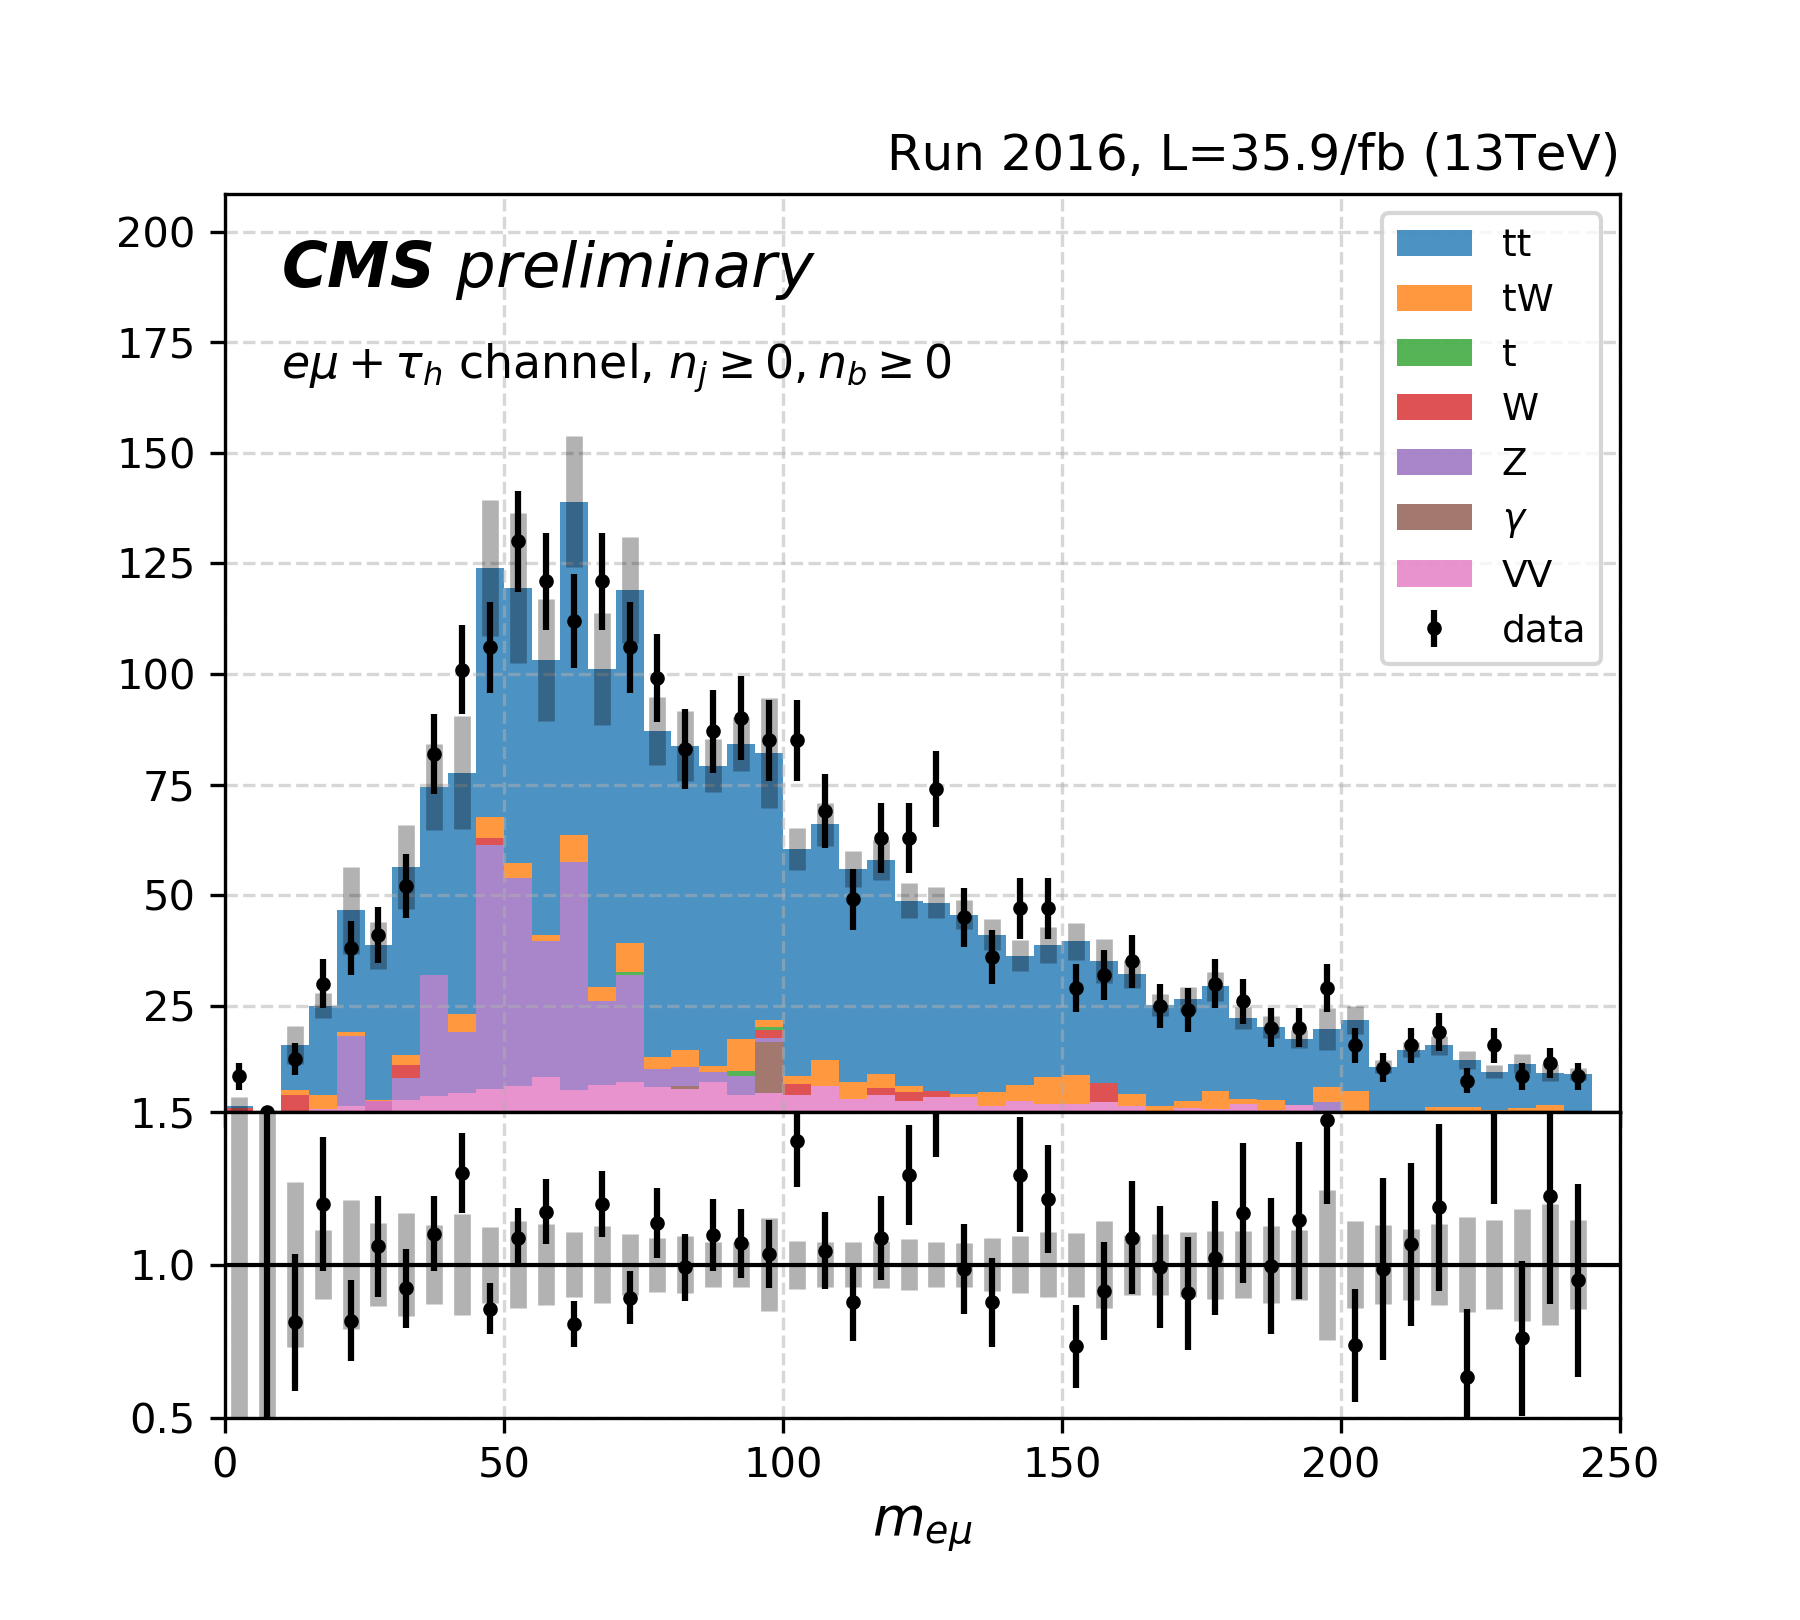
\includegraphics[width=0.4\textwidth]{appendices/jetToTauhReweighting/figures/emutau_dilepton_mass_pickles_lltauTight.png}
    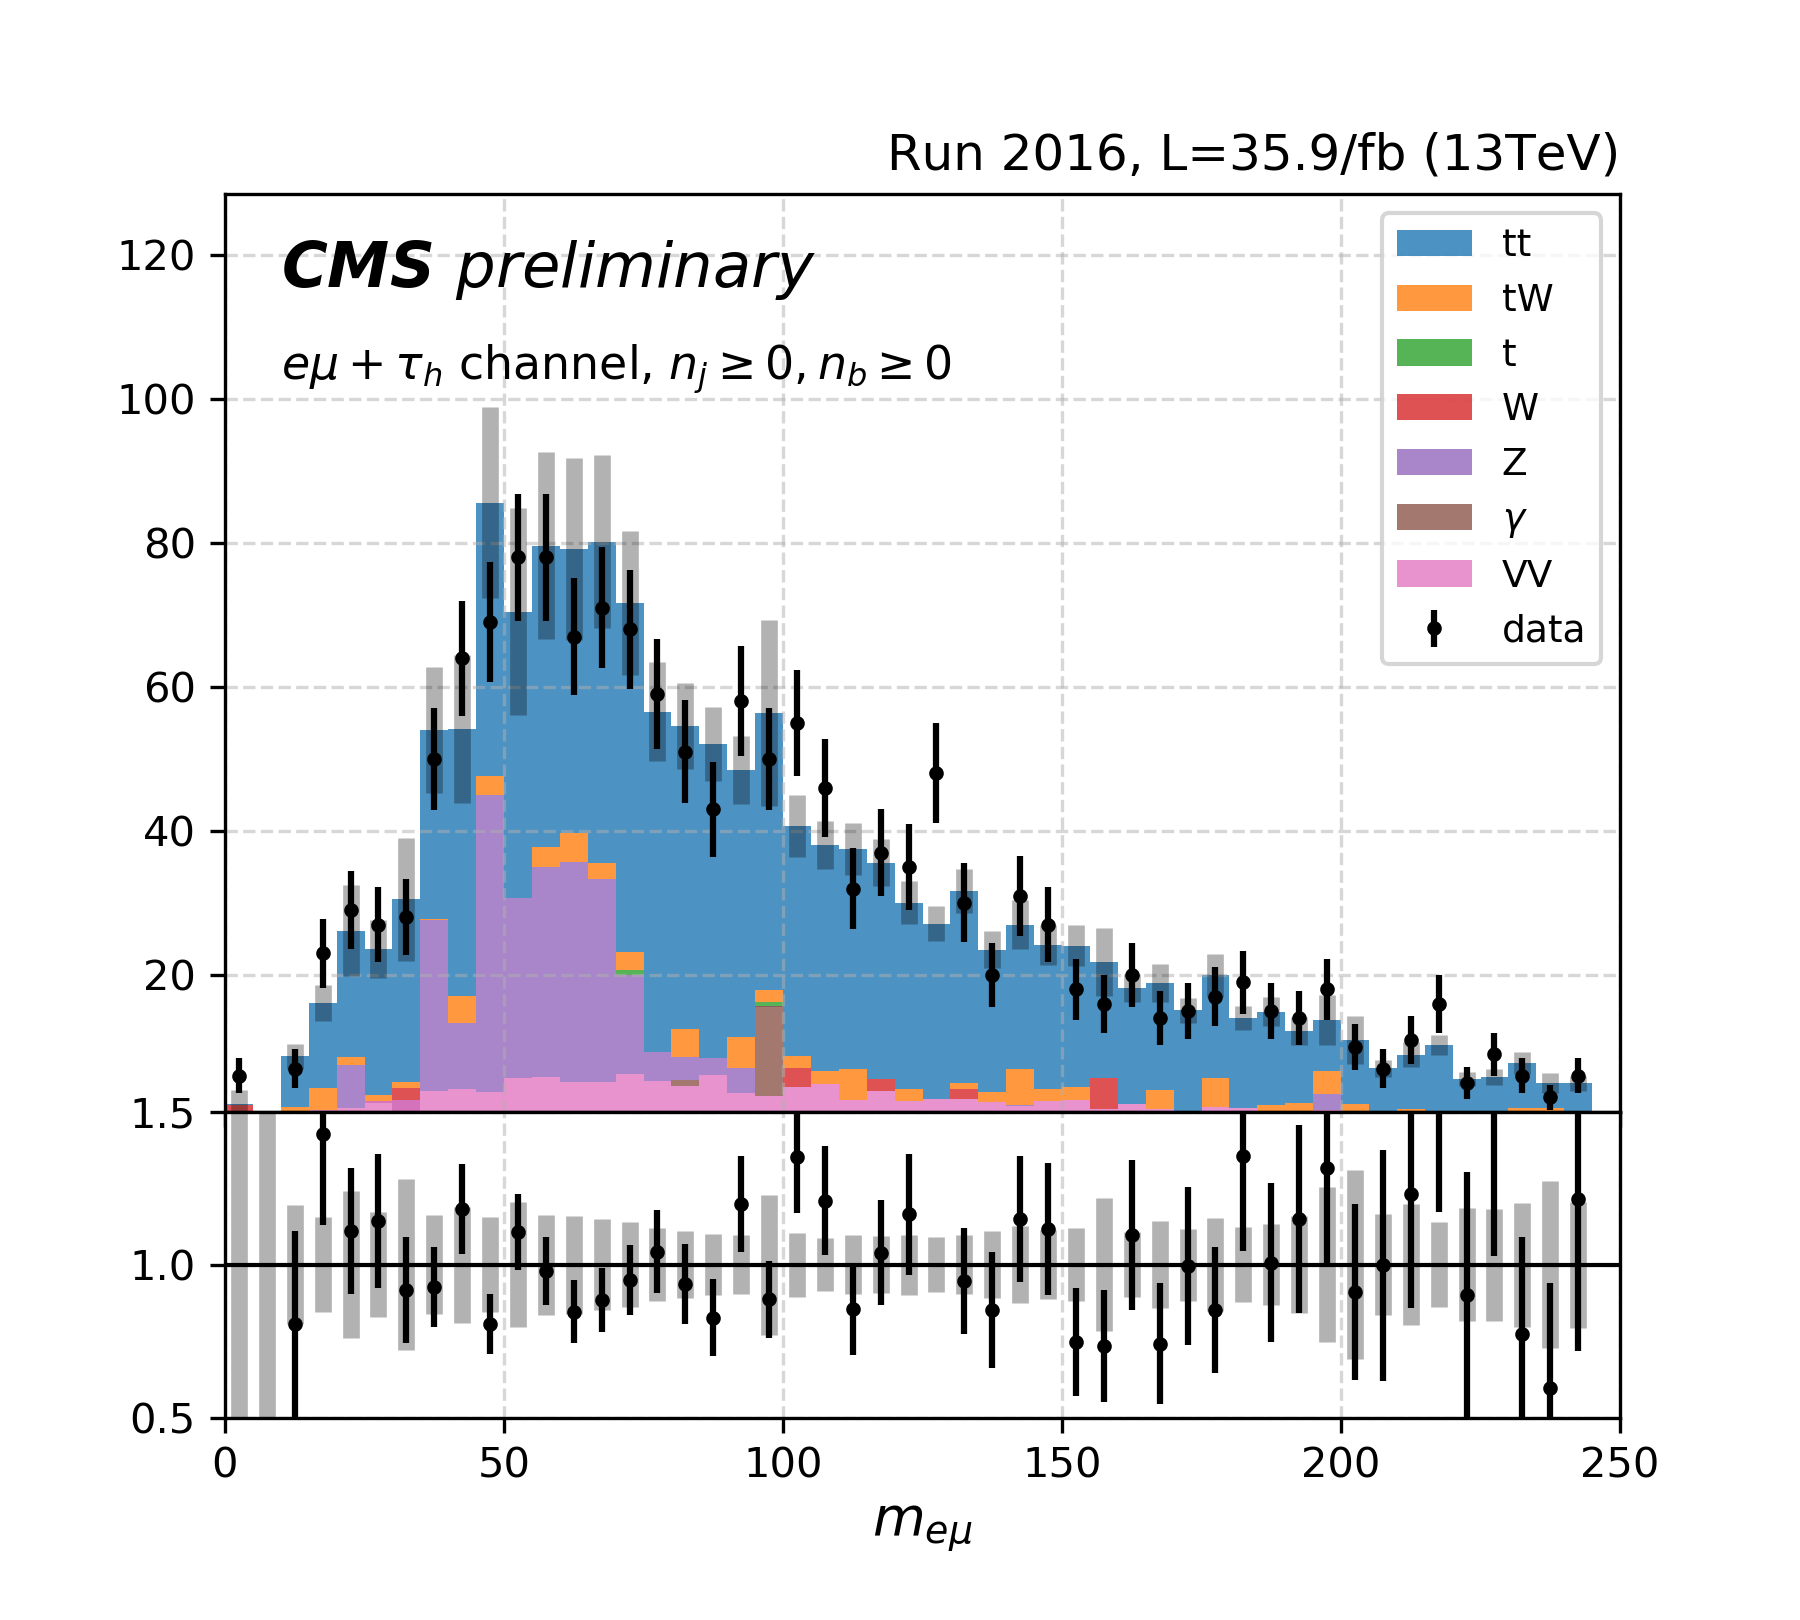
\includegraphics[width=0.4\textwidth]{appendices/jetToTauhReweighting/figures/emutau_dilepton_mass_pickles_lltauVTight.png}
    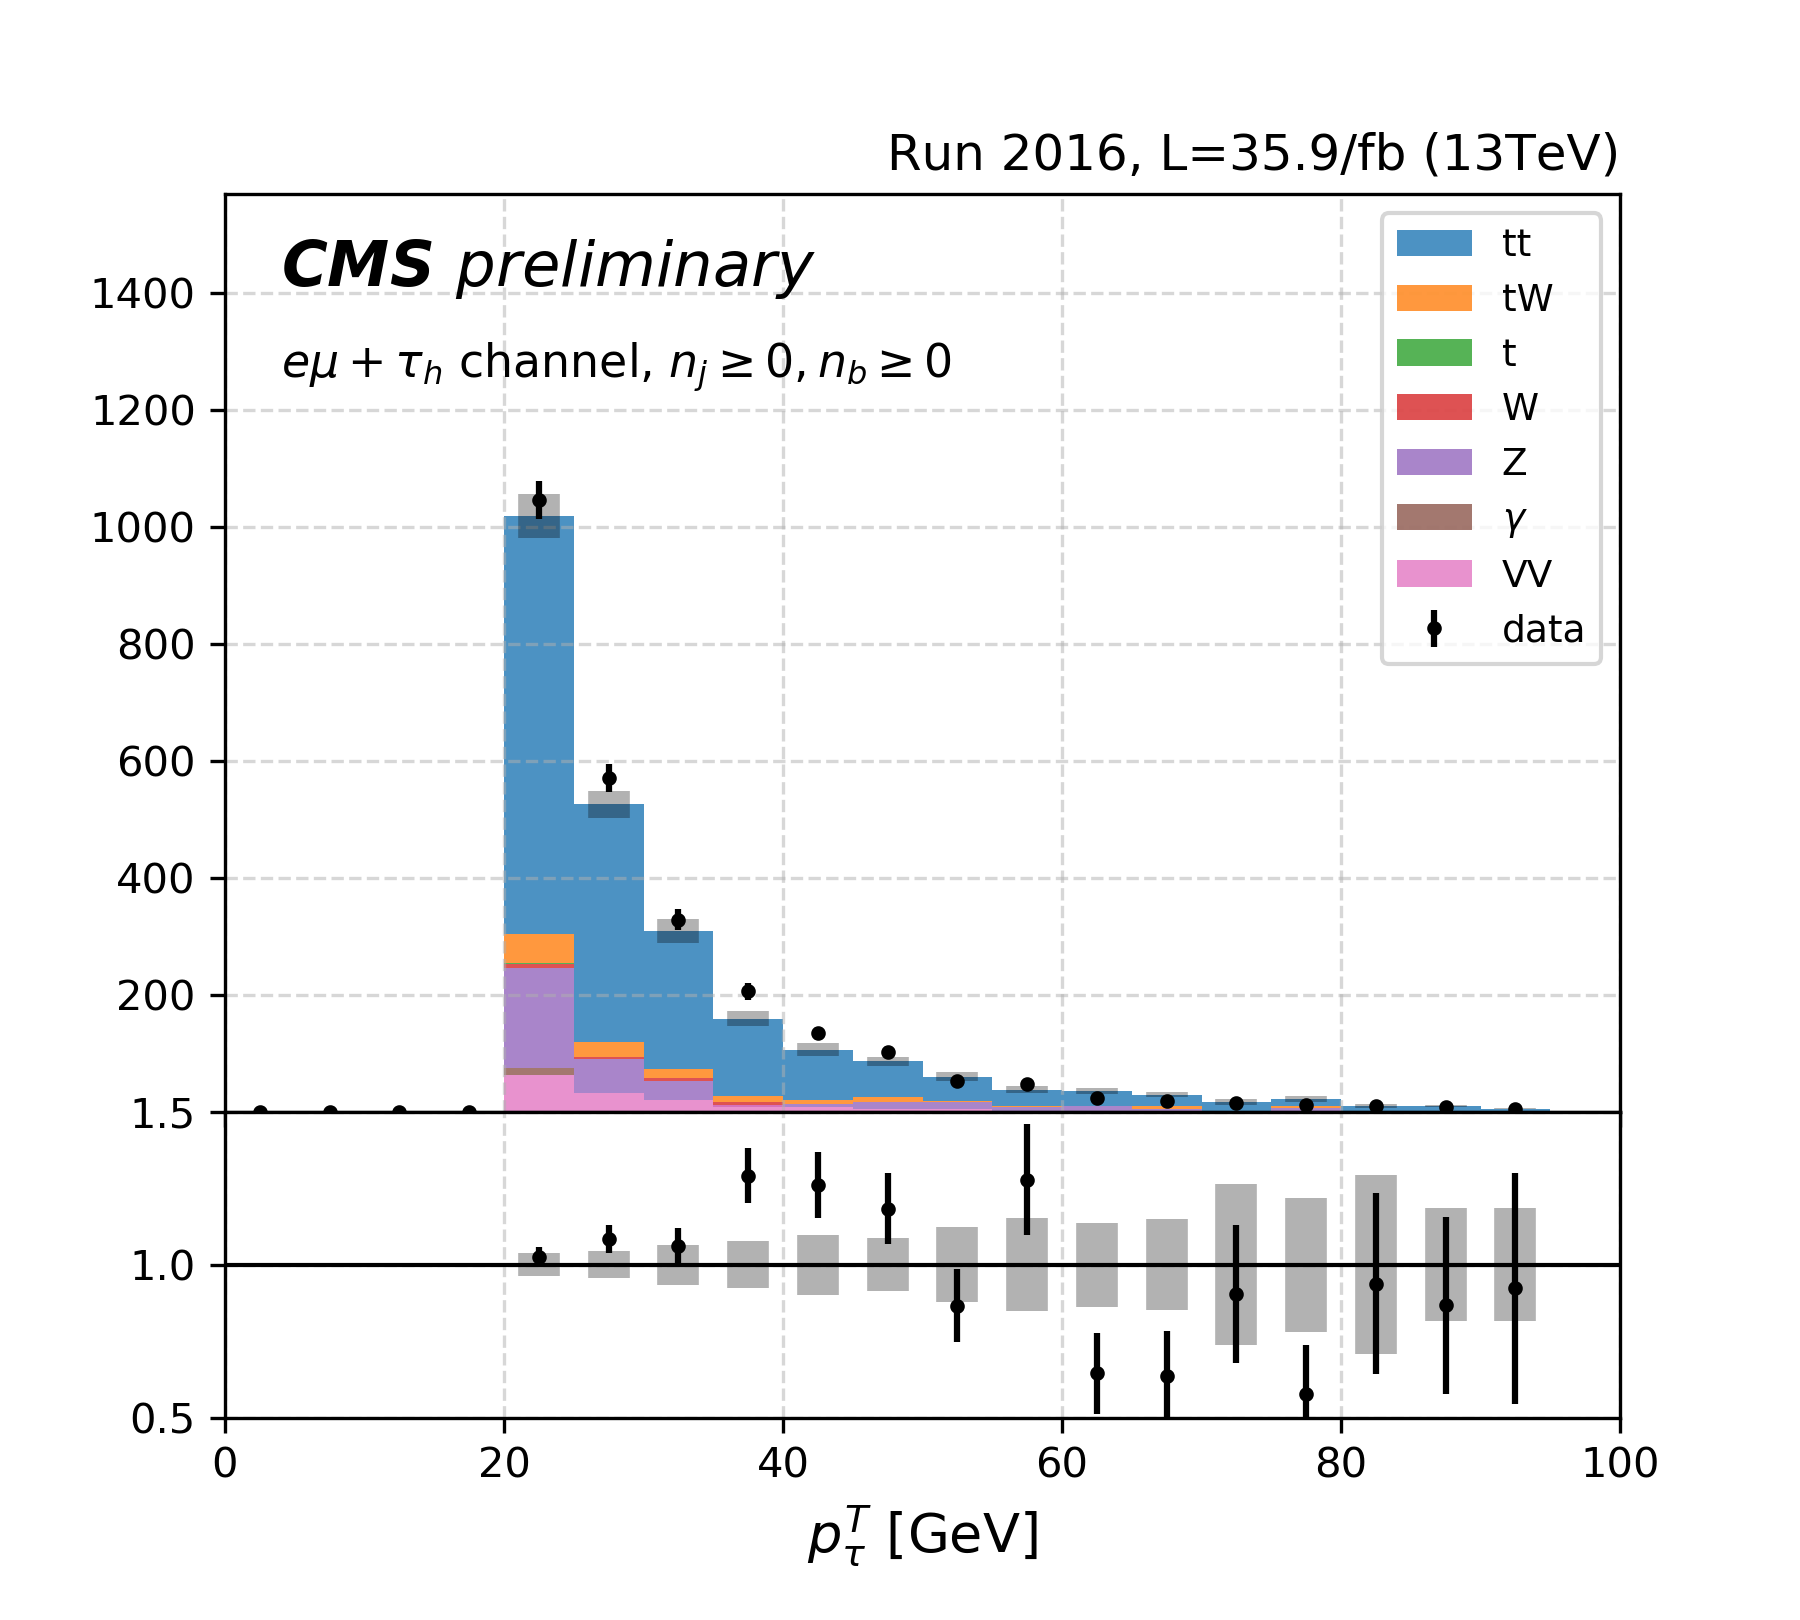
\includegraphics[width=0.4\textwidth]{appendices/jetToTauhReweighting/figures/emutau_tauPt_pickles_lltauTight.png}
    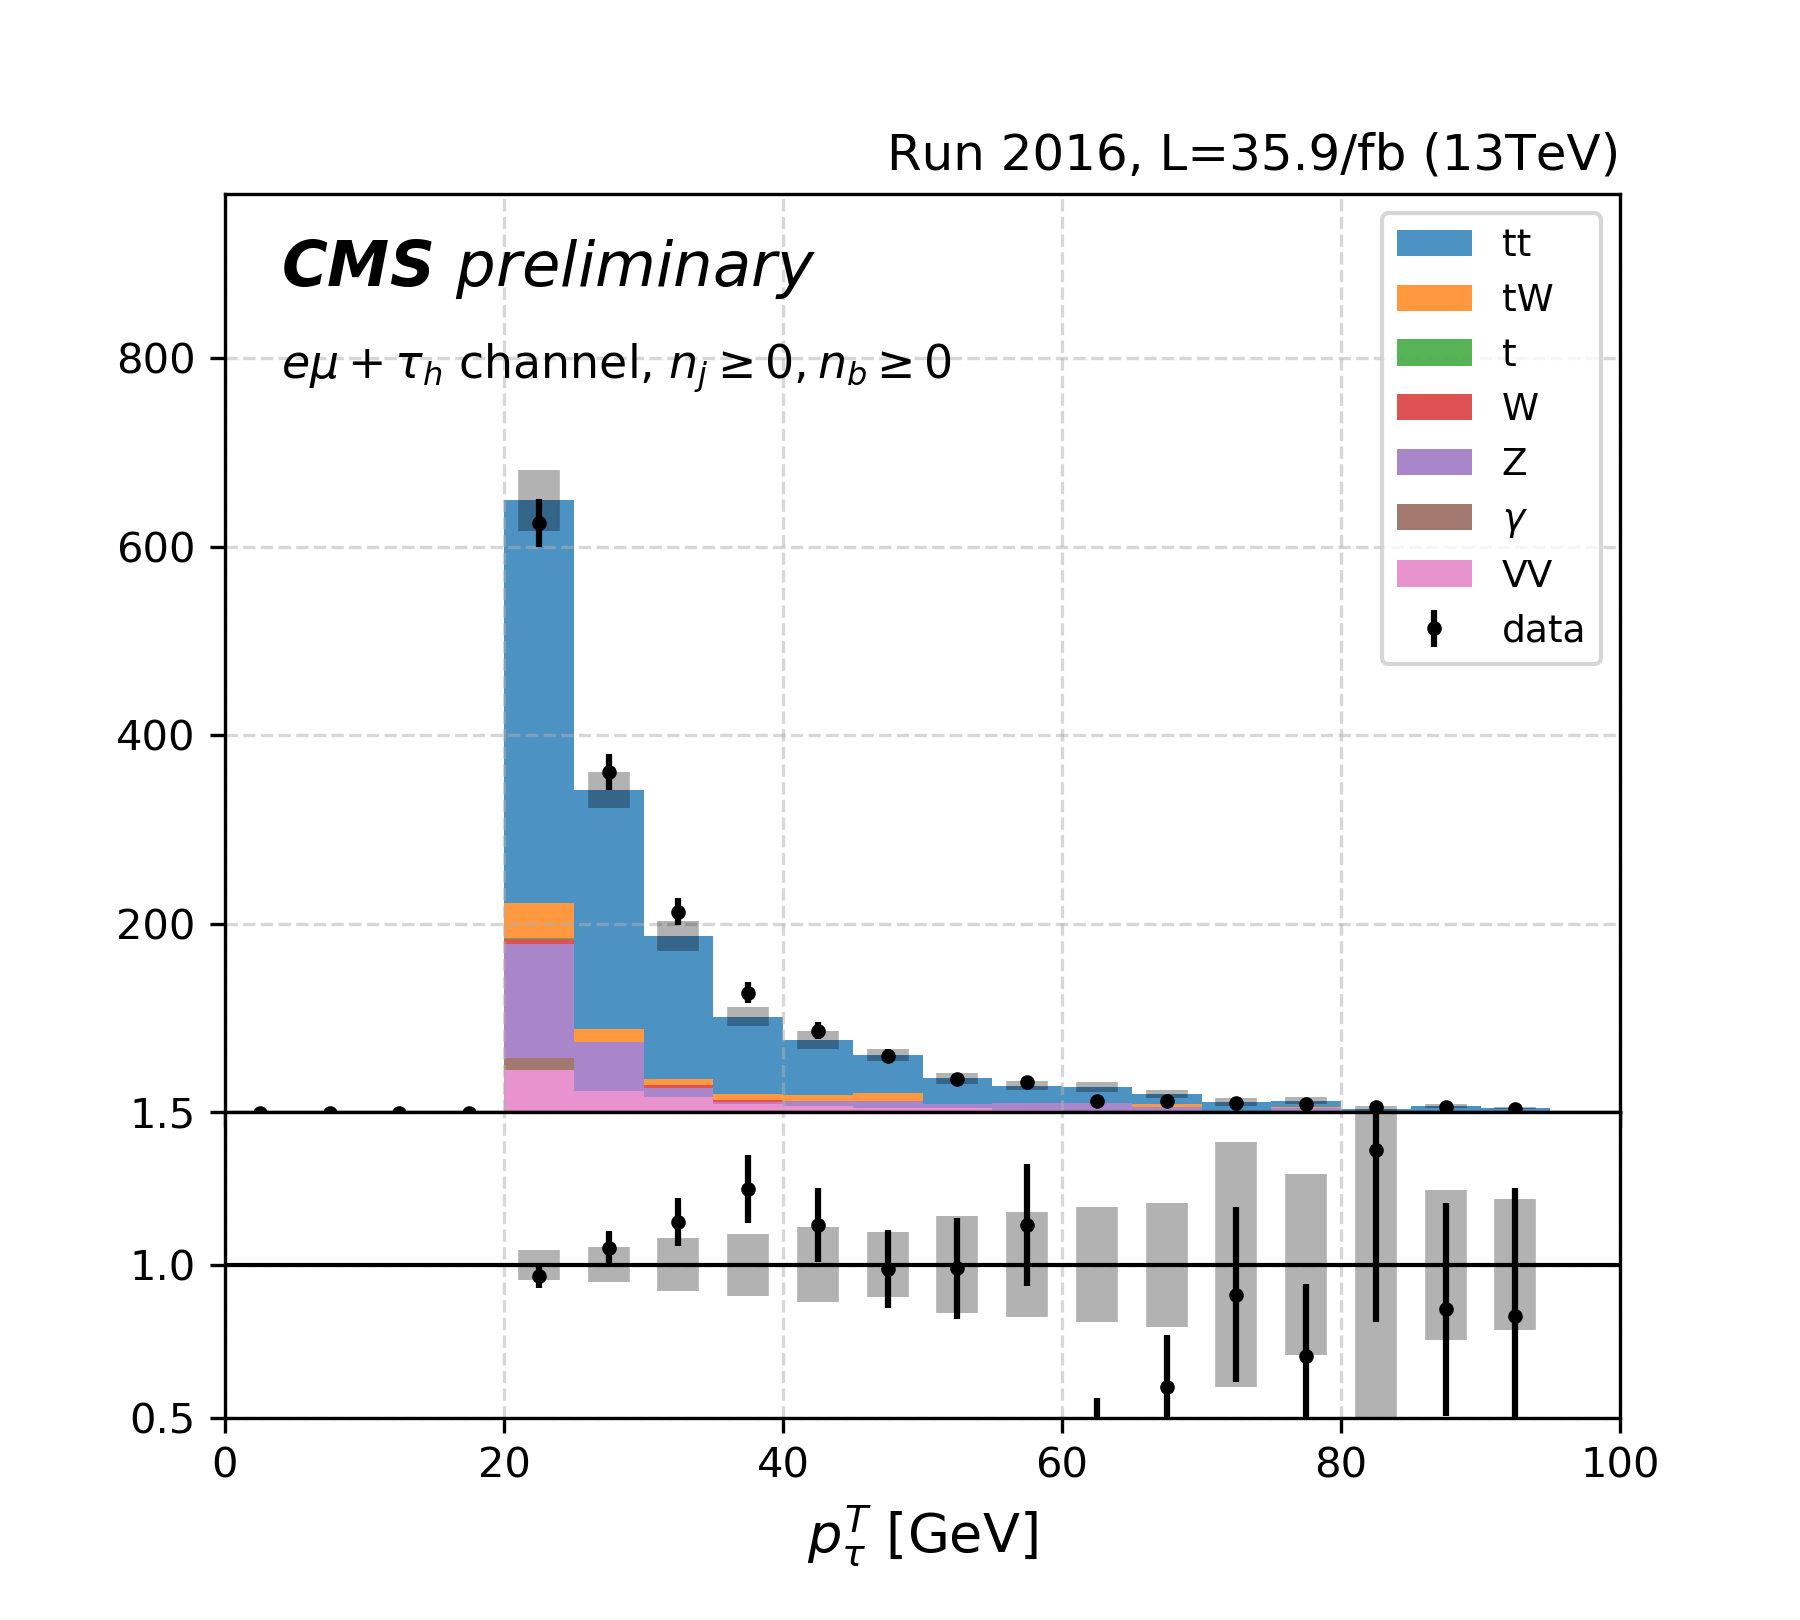
\includegraphics[width=0.4\textwidth]{appendices/jetToTauhReweighting/figures/emutau_tauPt_pickles_lltauVTight.png}
    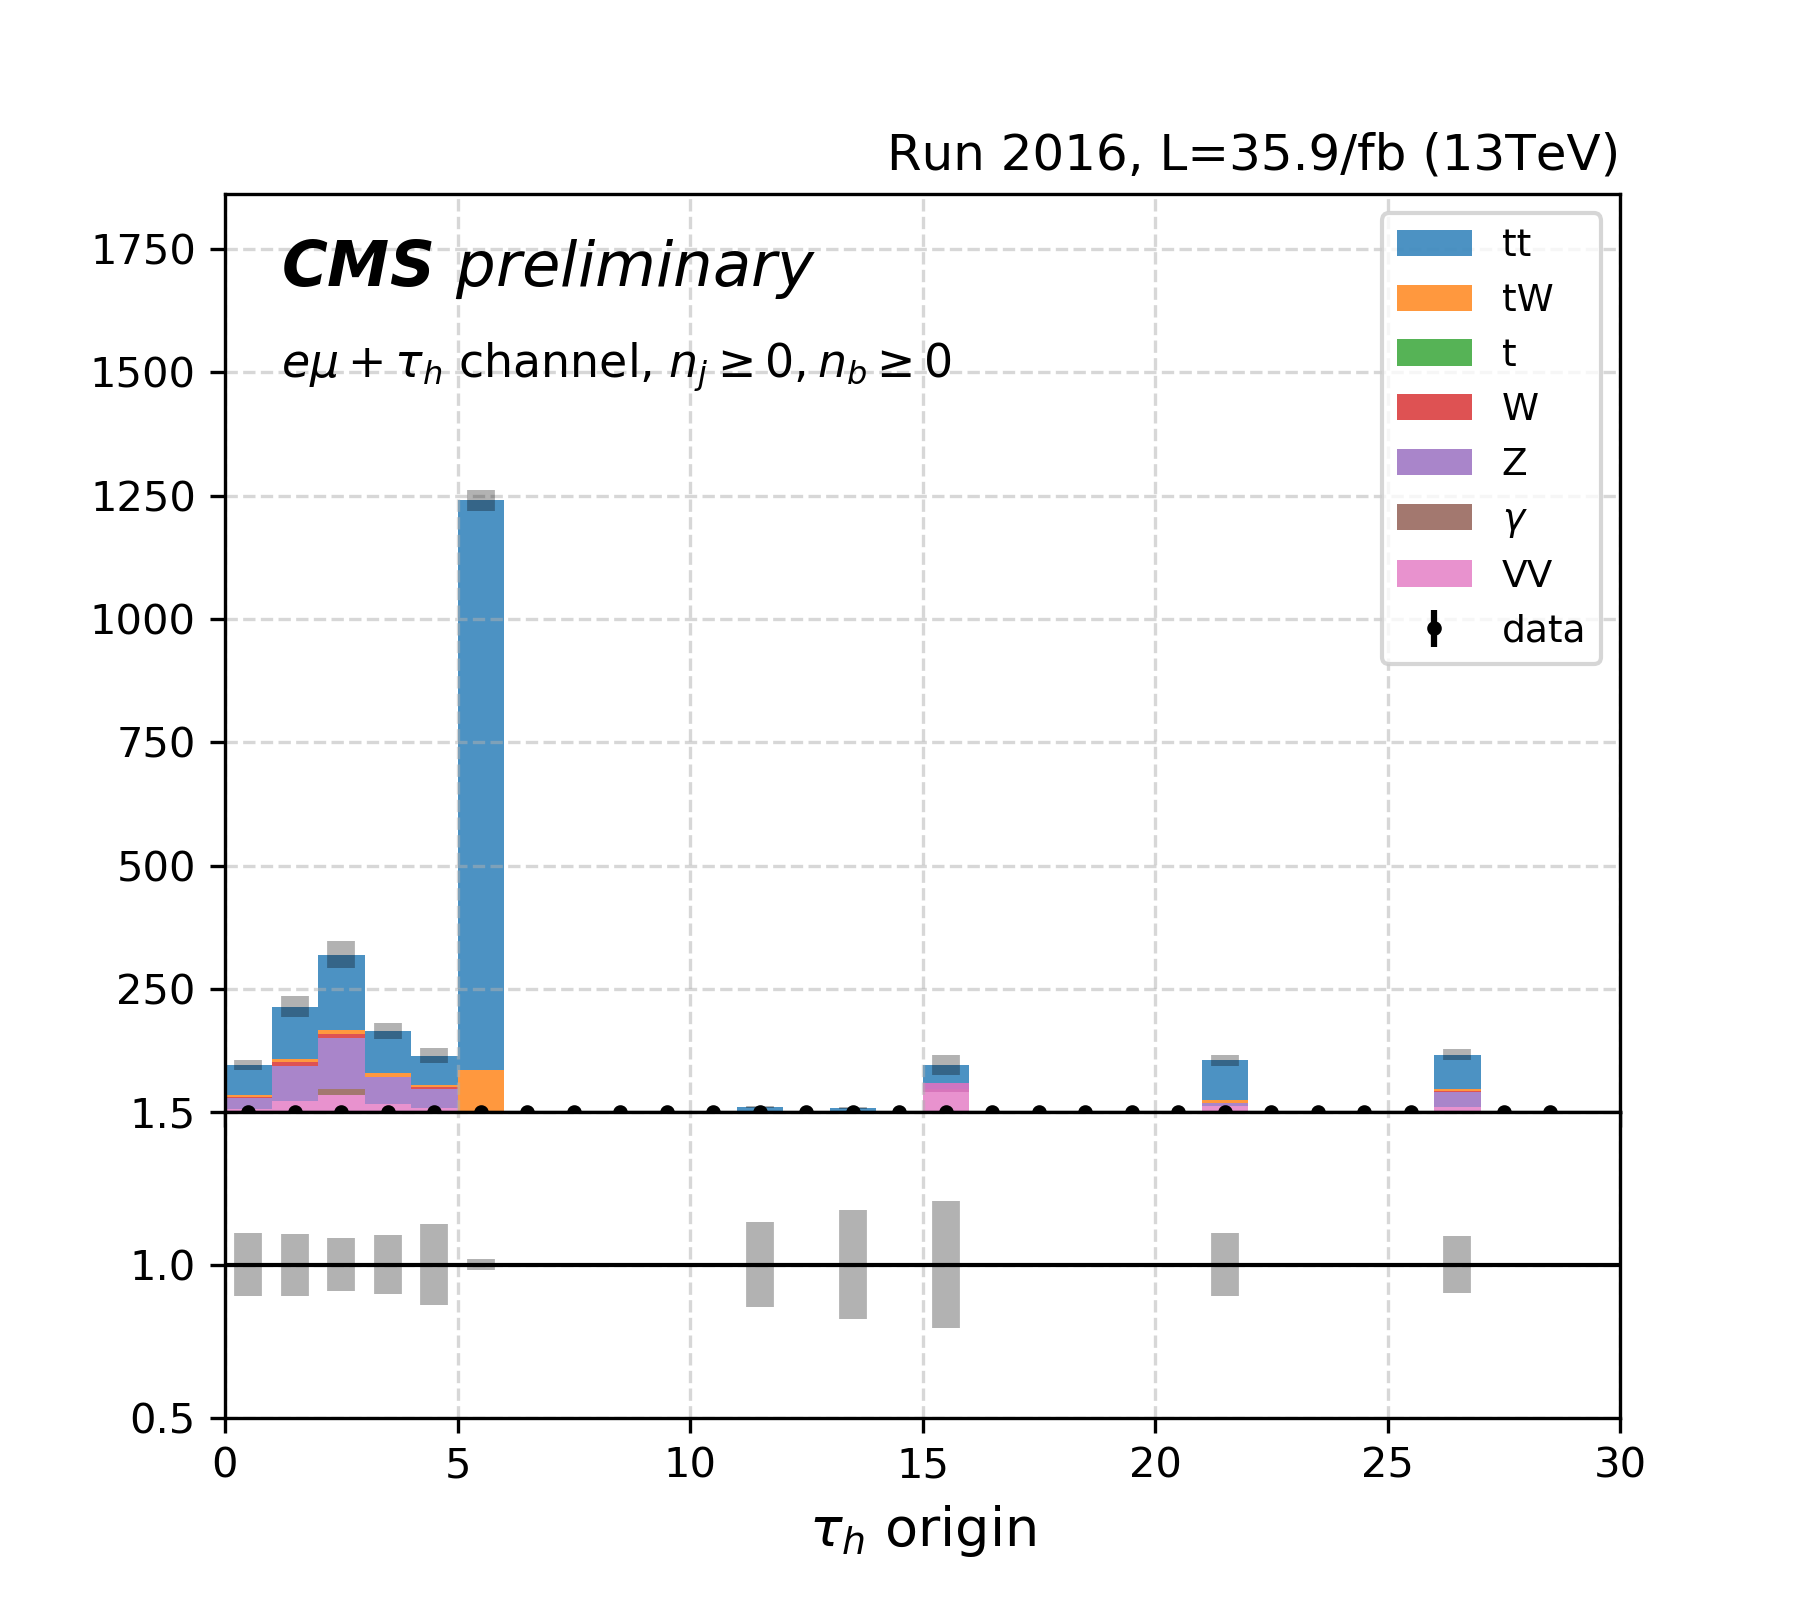
\includegraphics[width=0.4\textwidth]{appendices/jetToTauhReweighting/figures/emutau_tauGenFlavor_pickles_lltauTight.png}
    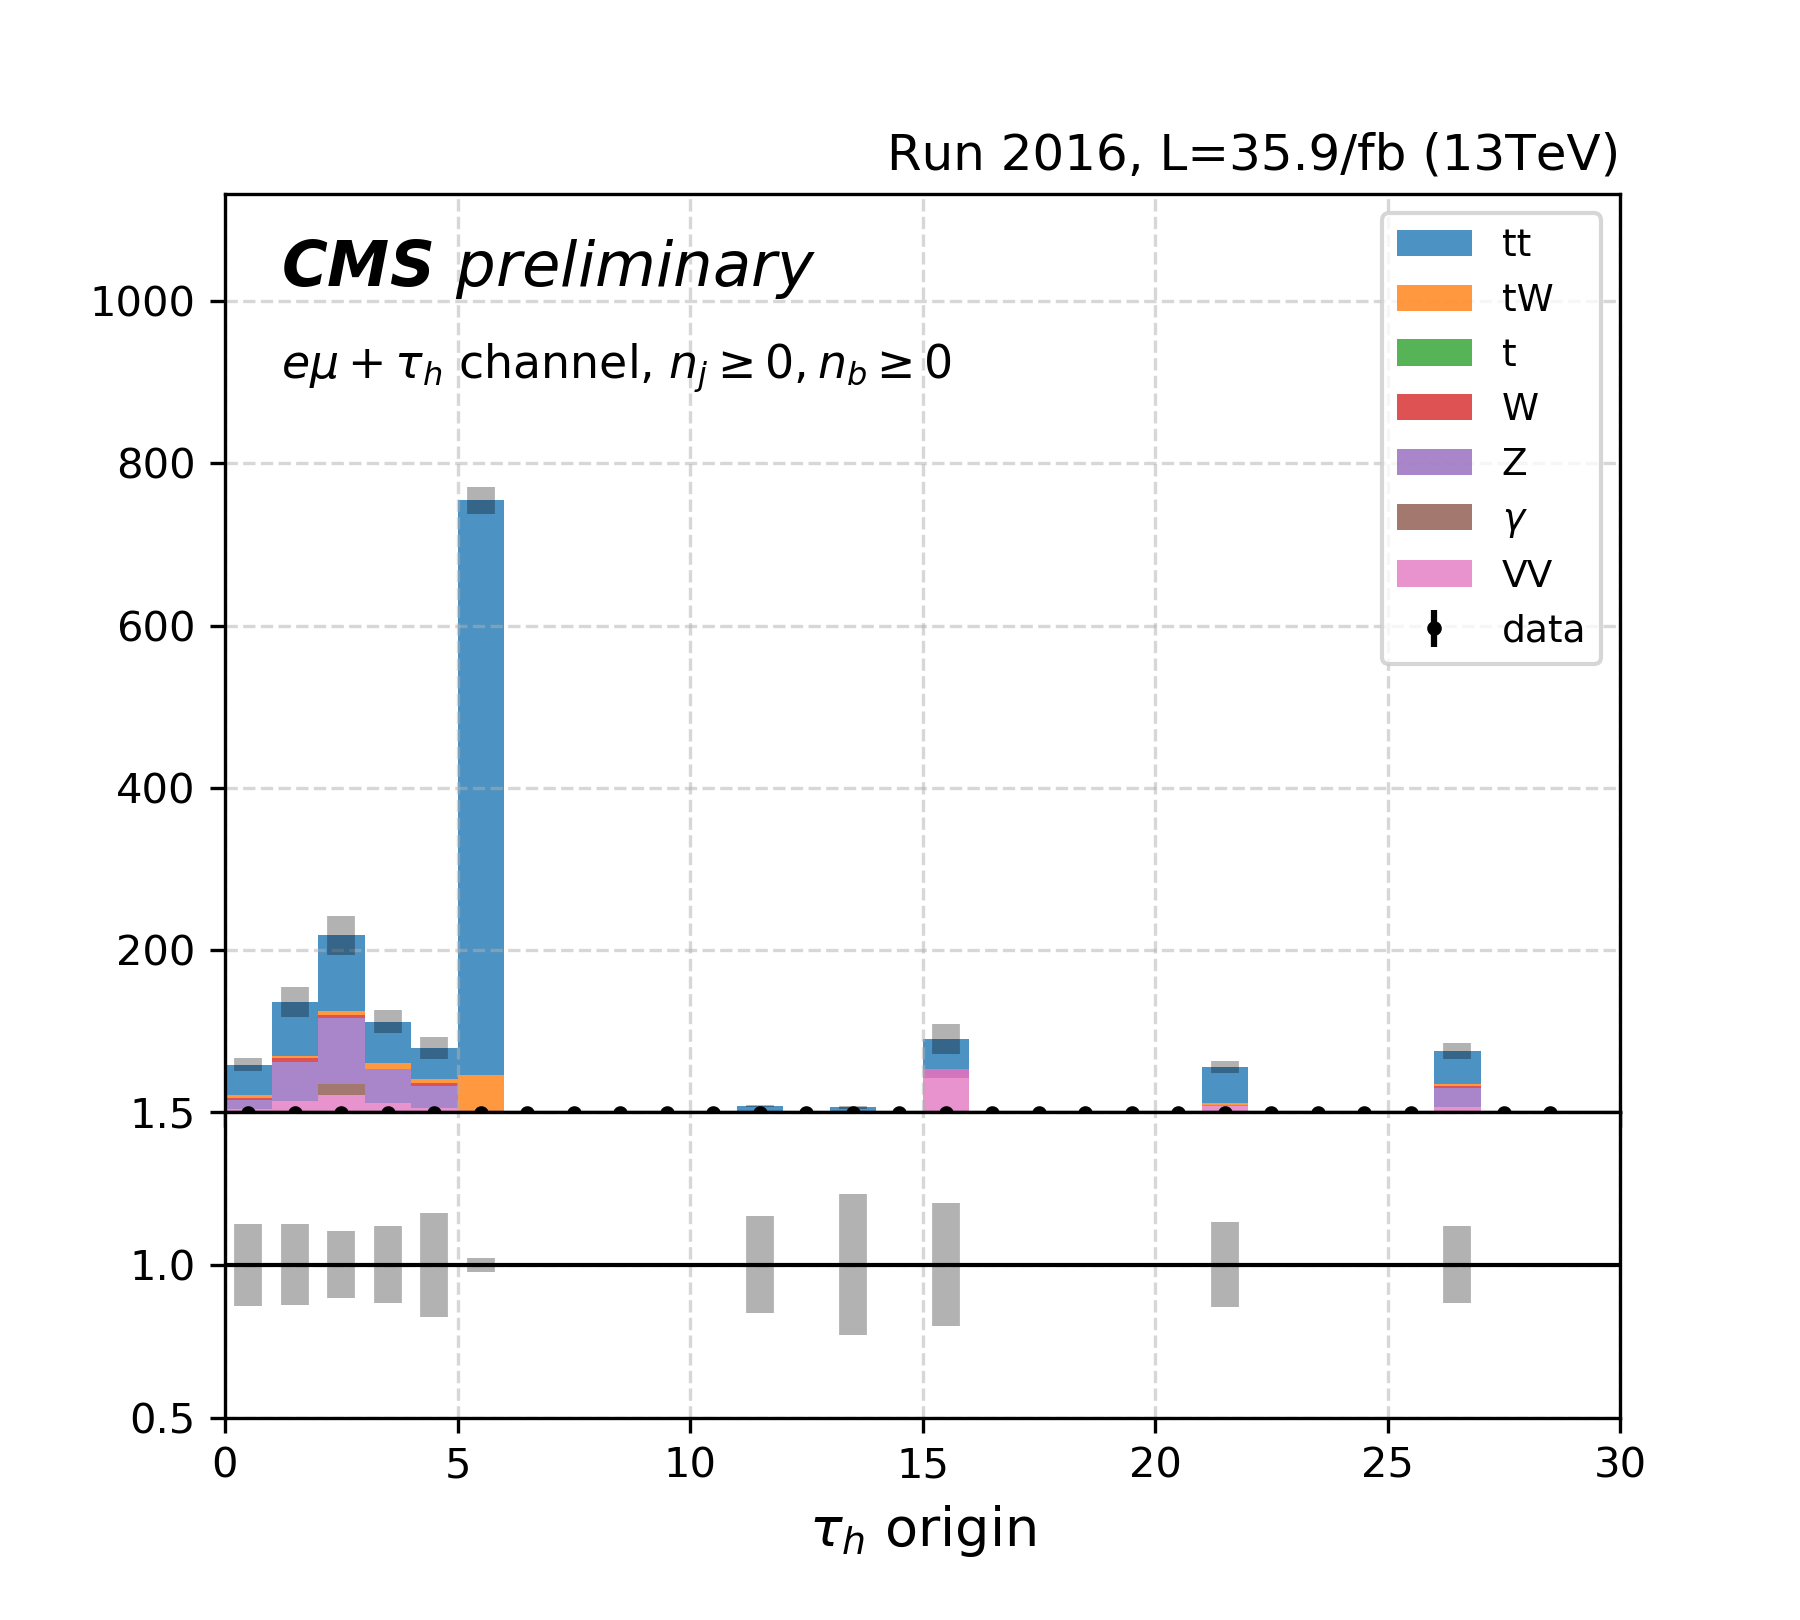
\includegraphics[width=0.4\textwidth]{appendices/jetToTauhReweighting/figures/emutau_tauGenFlavor_pickles_lltauVTight.png}
    \caption{Distributions of $m_{e\mu}$, $\tau pT$ and gen-level $\tau_h$ origin in the $e\mu+\tau$ channel. The left and right column shows the Tight and VTight $\tau_h$ WP respectively.}
    \label{fig:appendix:fakeTauId:emutau}
\end{figure}

\begin{figure}
    \centering
    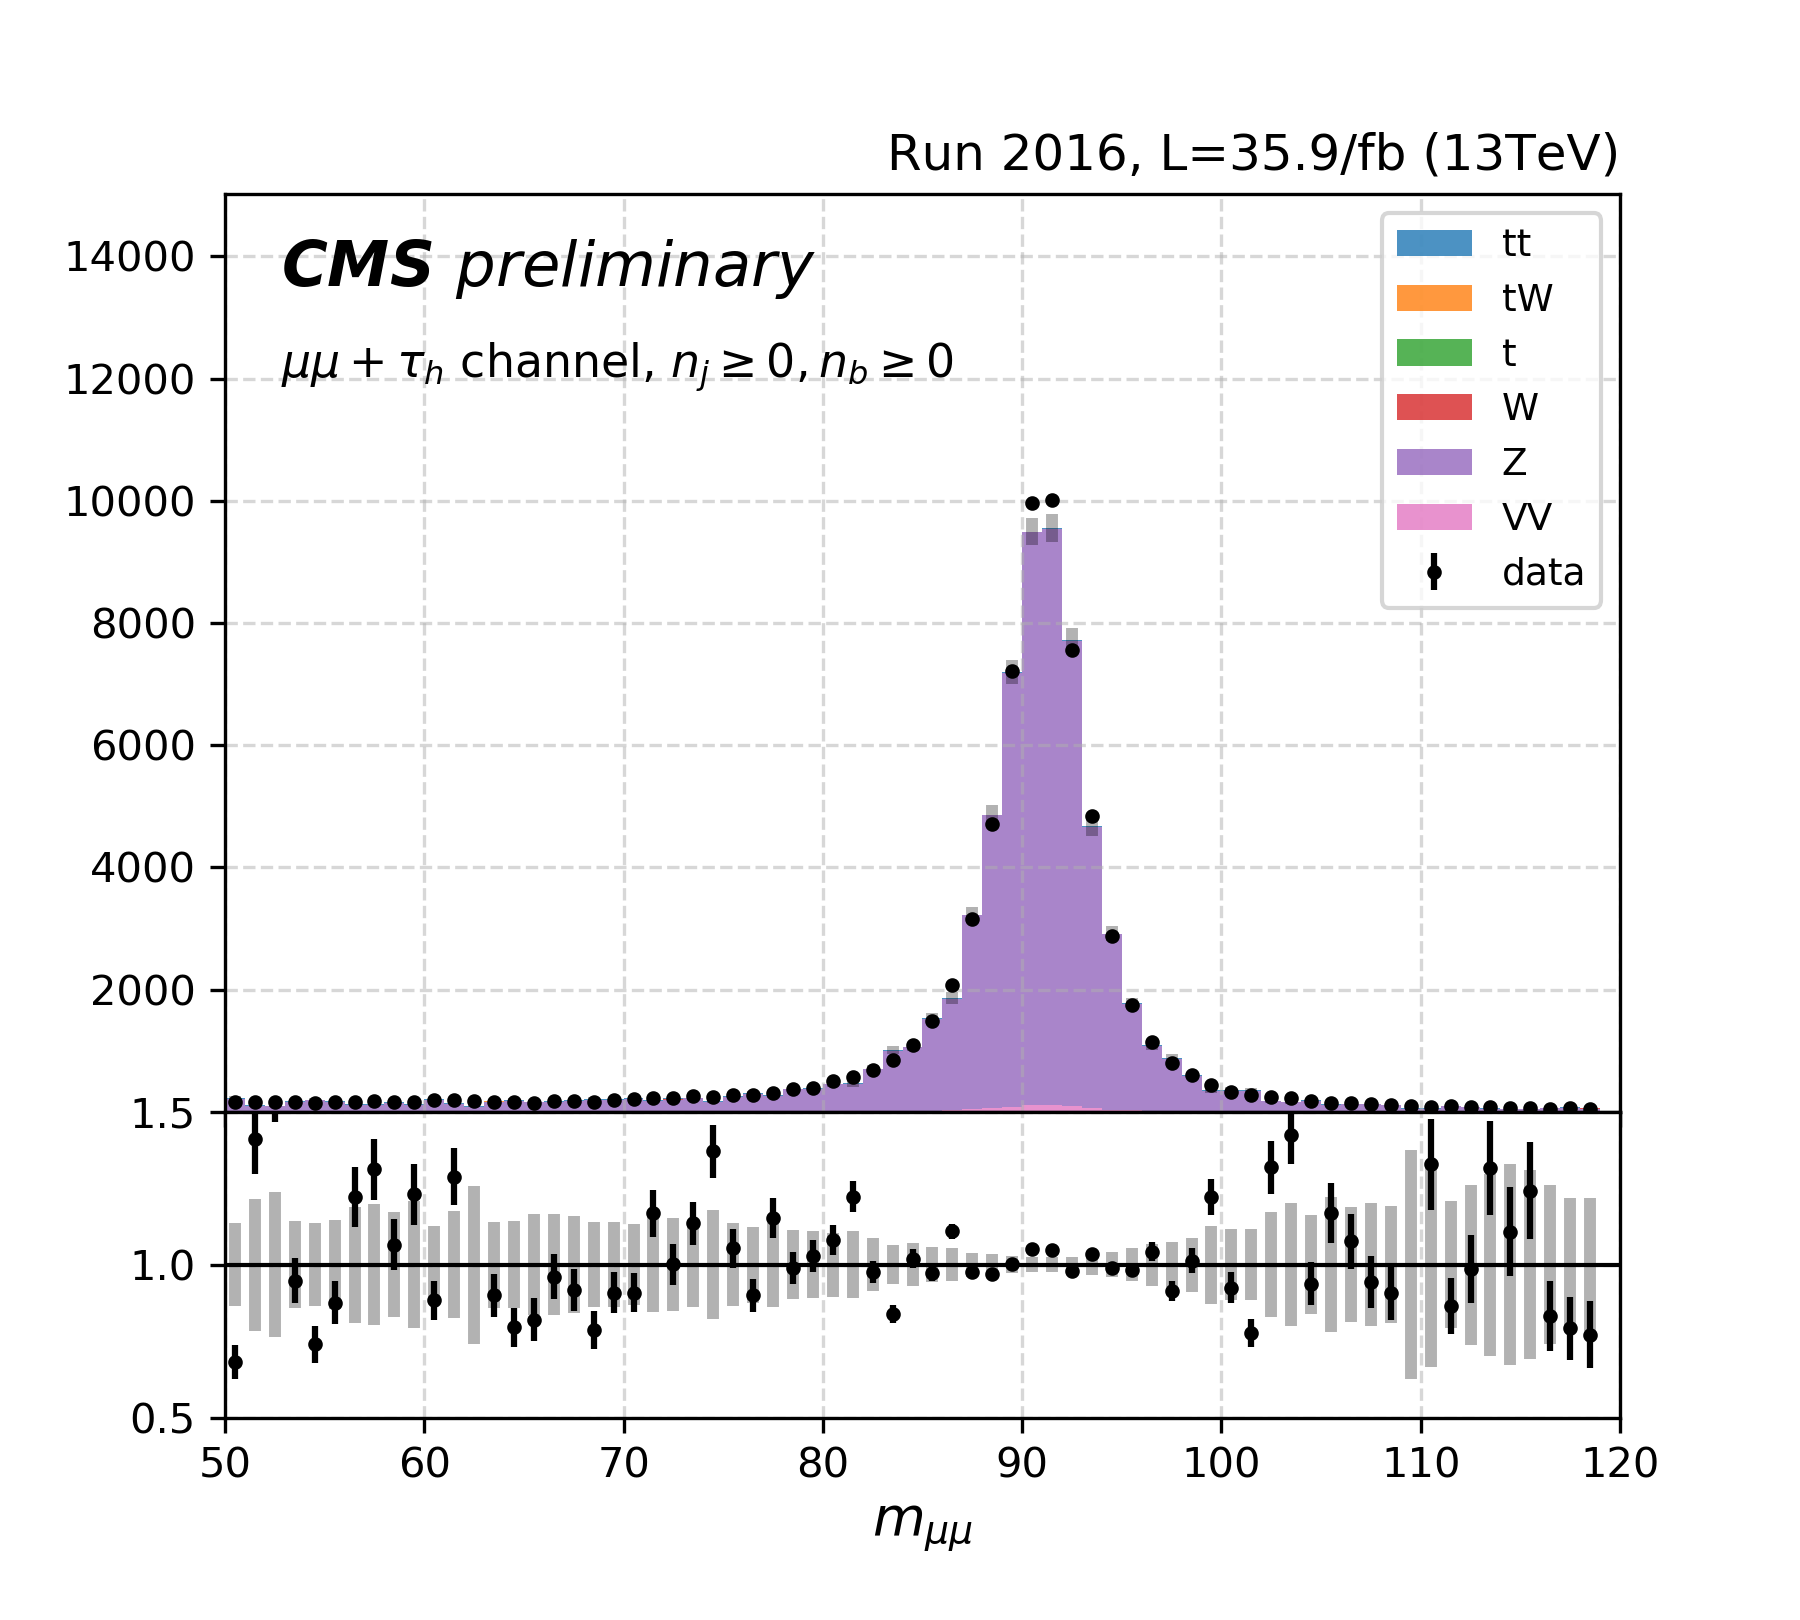
\includegraphics[width=0.4\textwidth]{appendices/jetToTauhReweighting/figures/mumutau_dilepton_mass_pickles_lltauTight.png}
    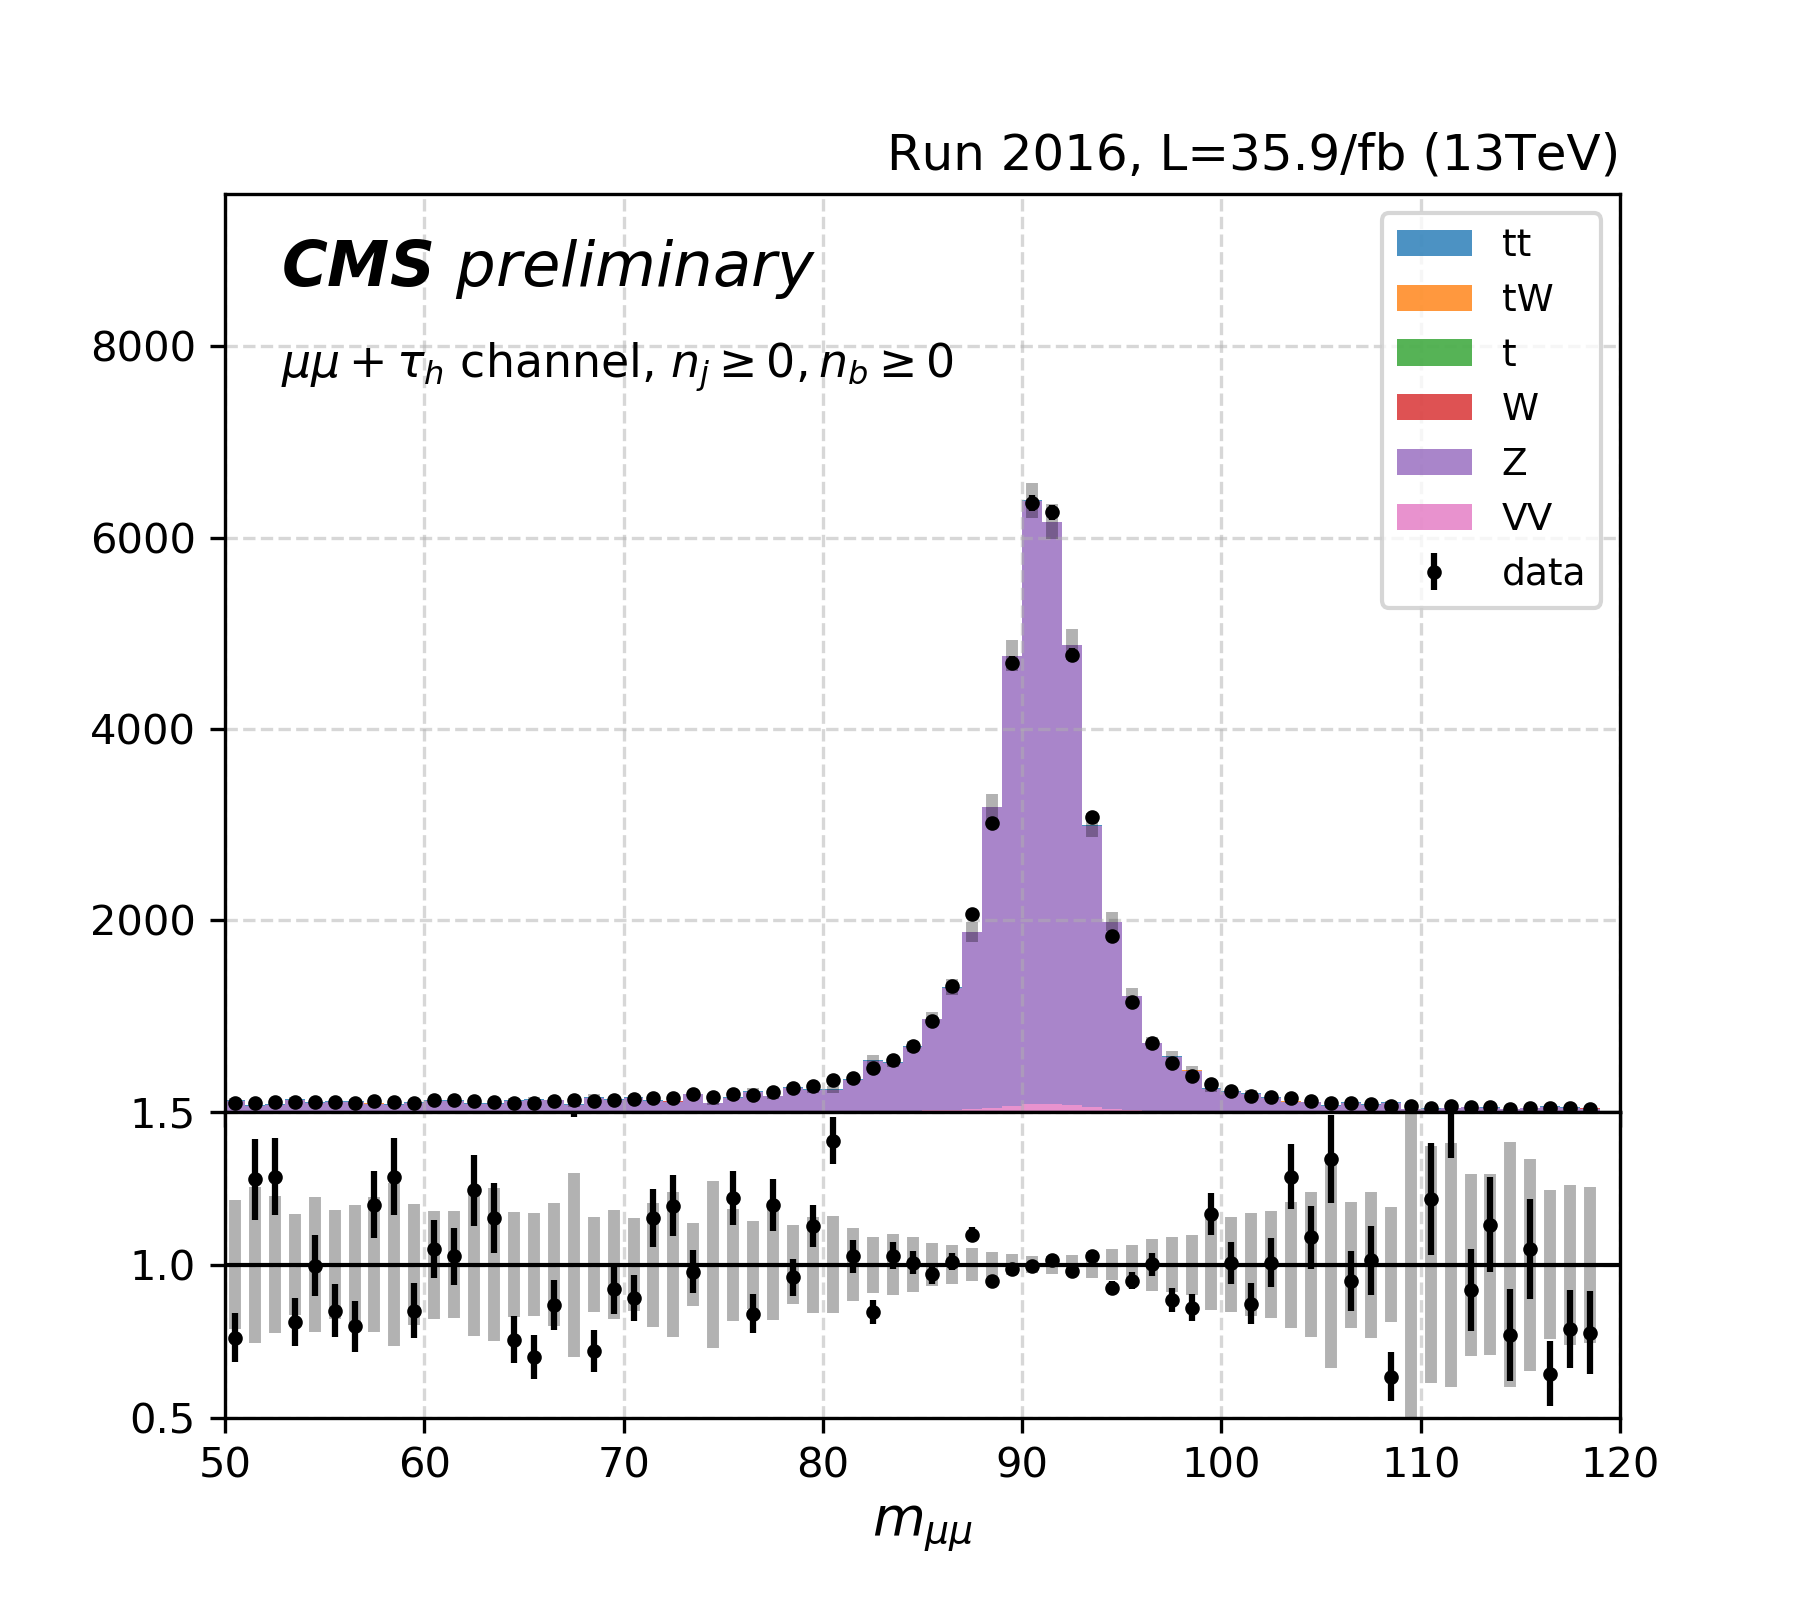
\includegraphics[width=0.4\textwidth]{appendices/jetToTauhReweighting/figures/mumutau_dilepton_mass_pickles_lltauVTight.png}
    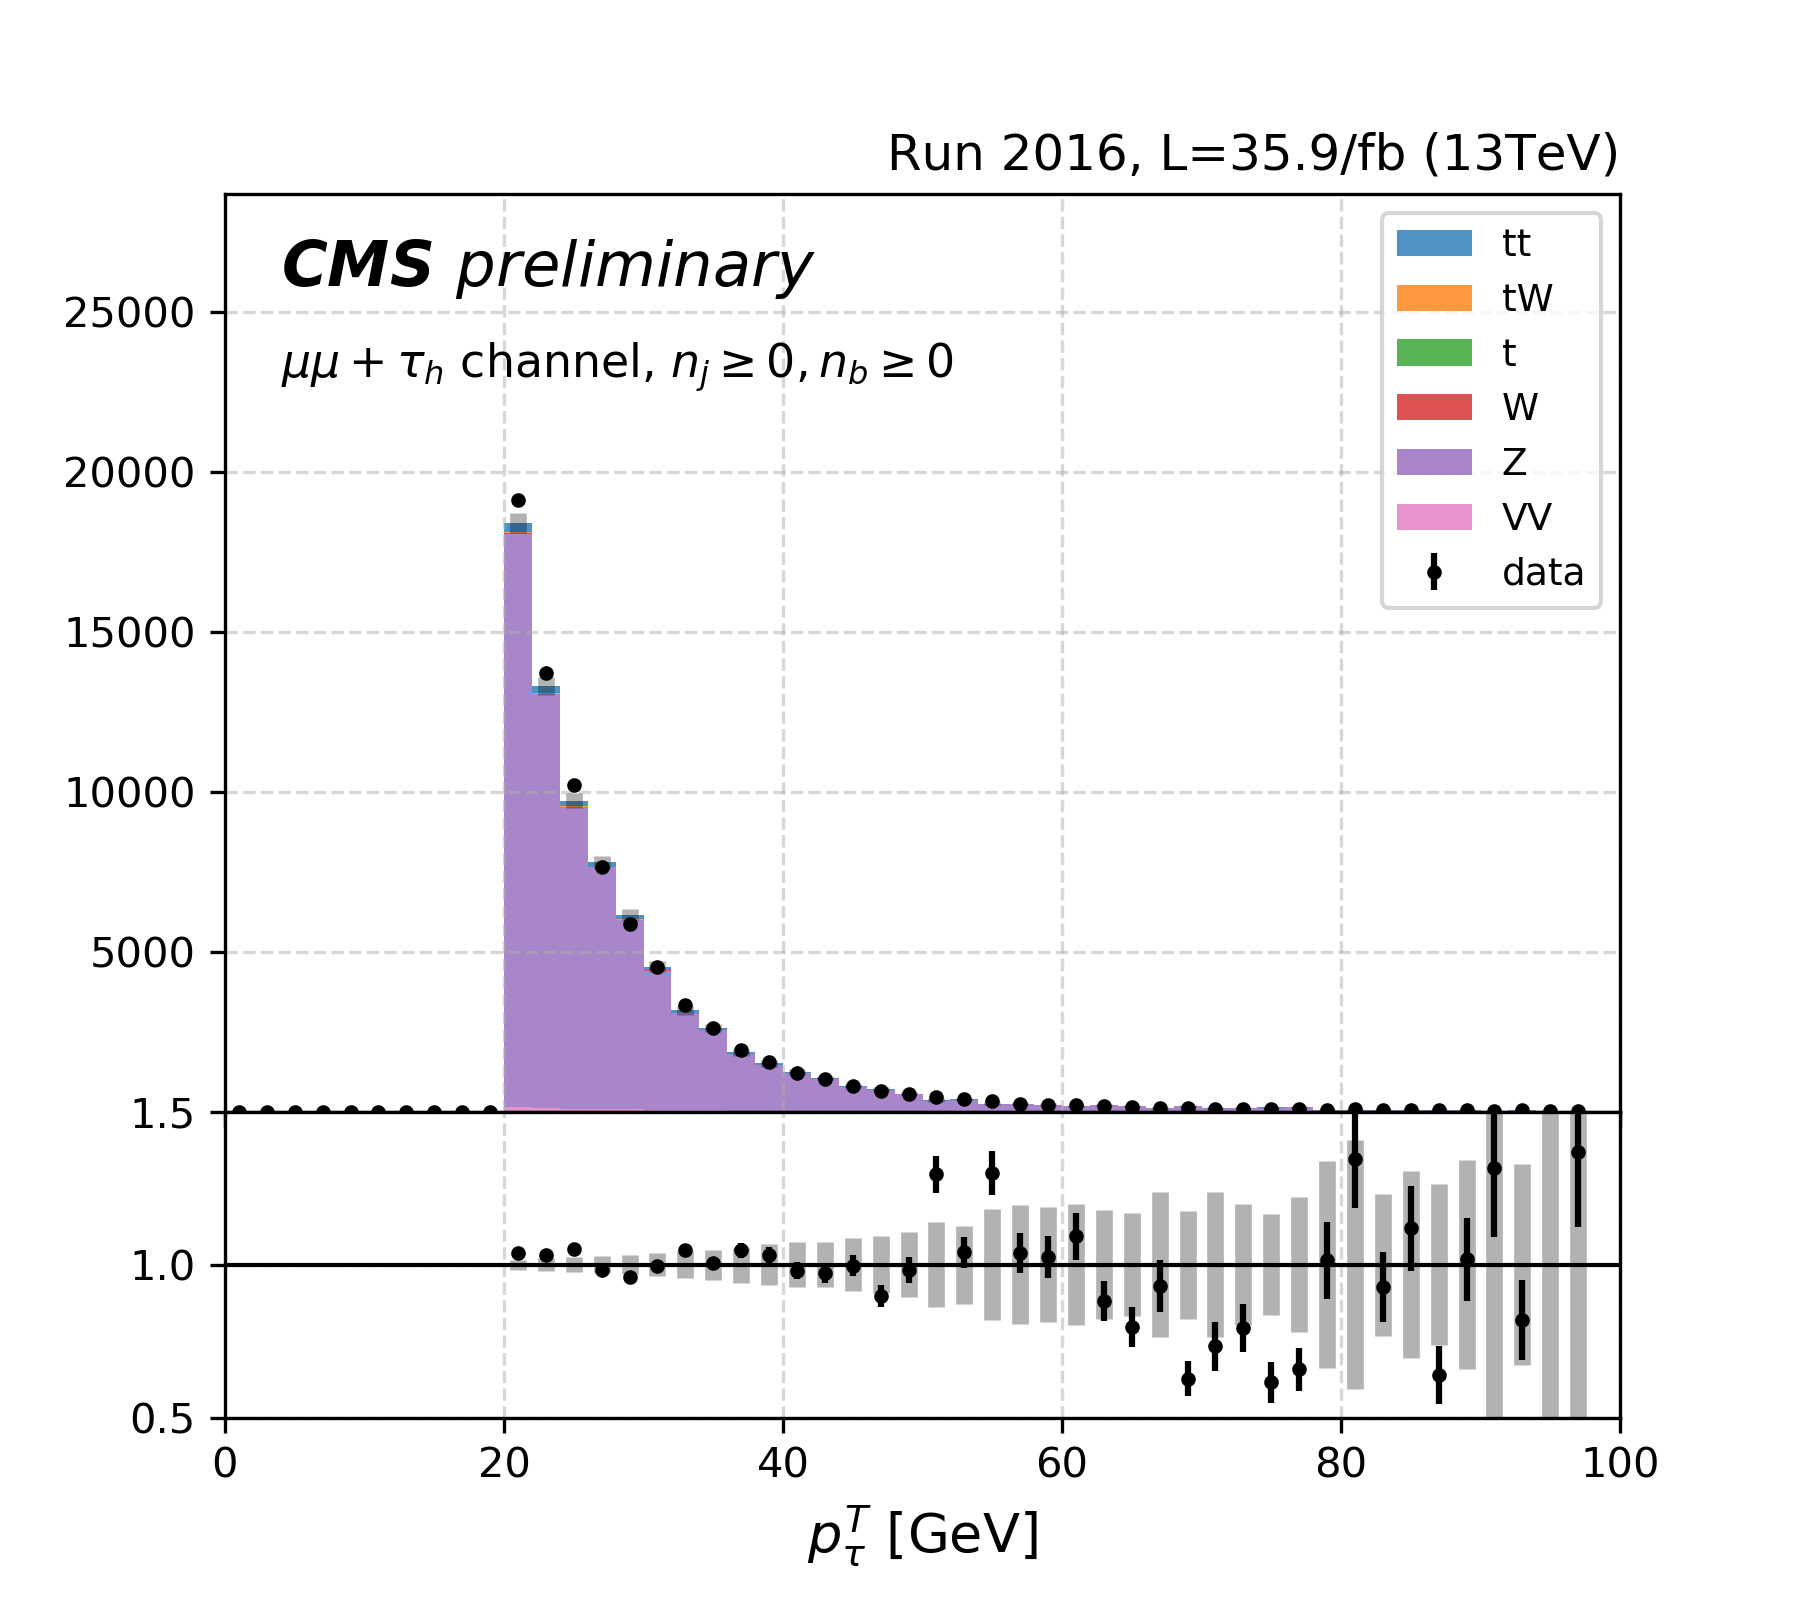
\includegraphics[width=0.4\textwidth]{appendices/jetToTauhReweighting/figures/mumutau_tauPt_pickles_lltauTight.png}
    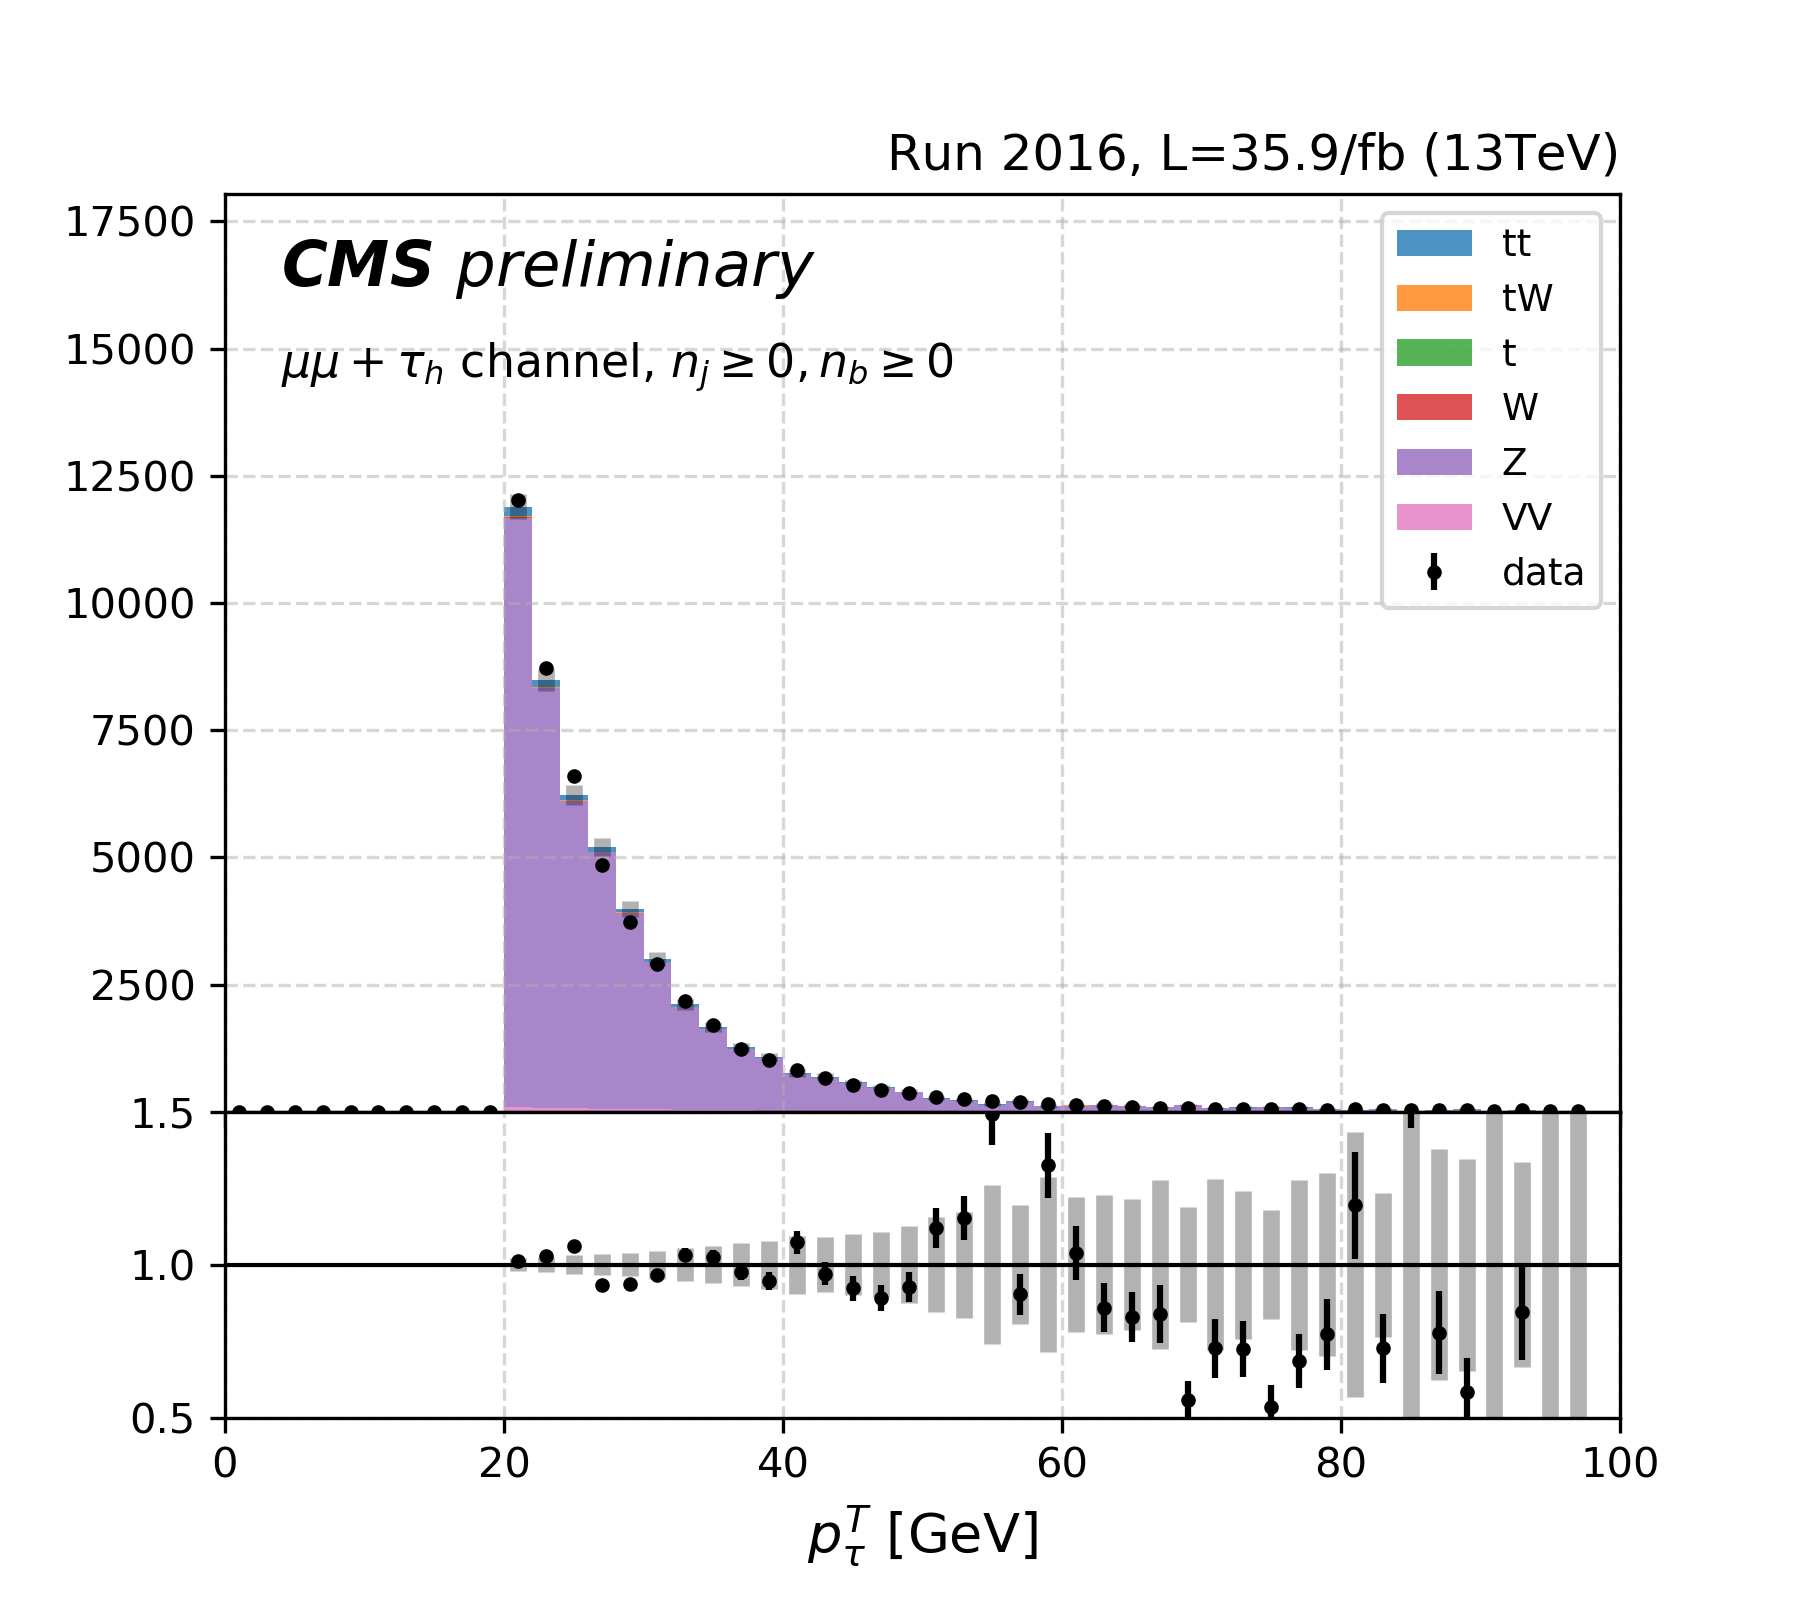
\includegraphics[width=0.4\textwidth]{appendices/jetToTauhReweighting/figures/mumutau_tauPt_pickles_lltauVTight.png}
    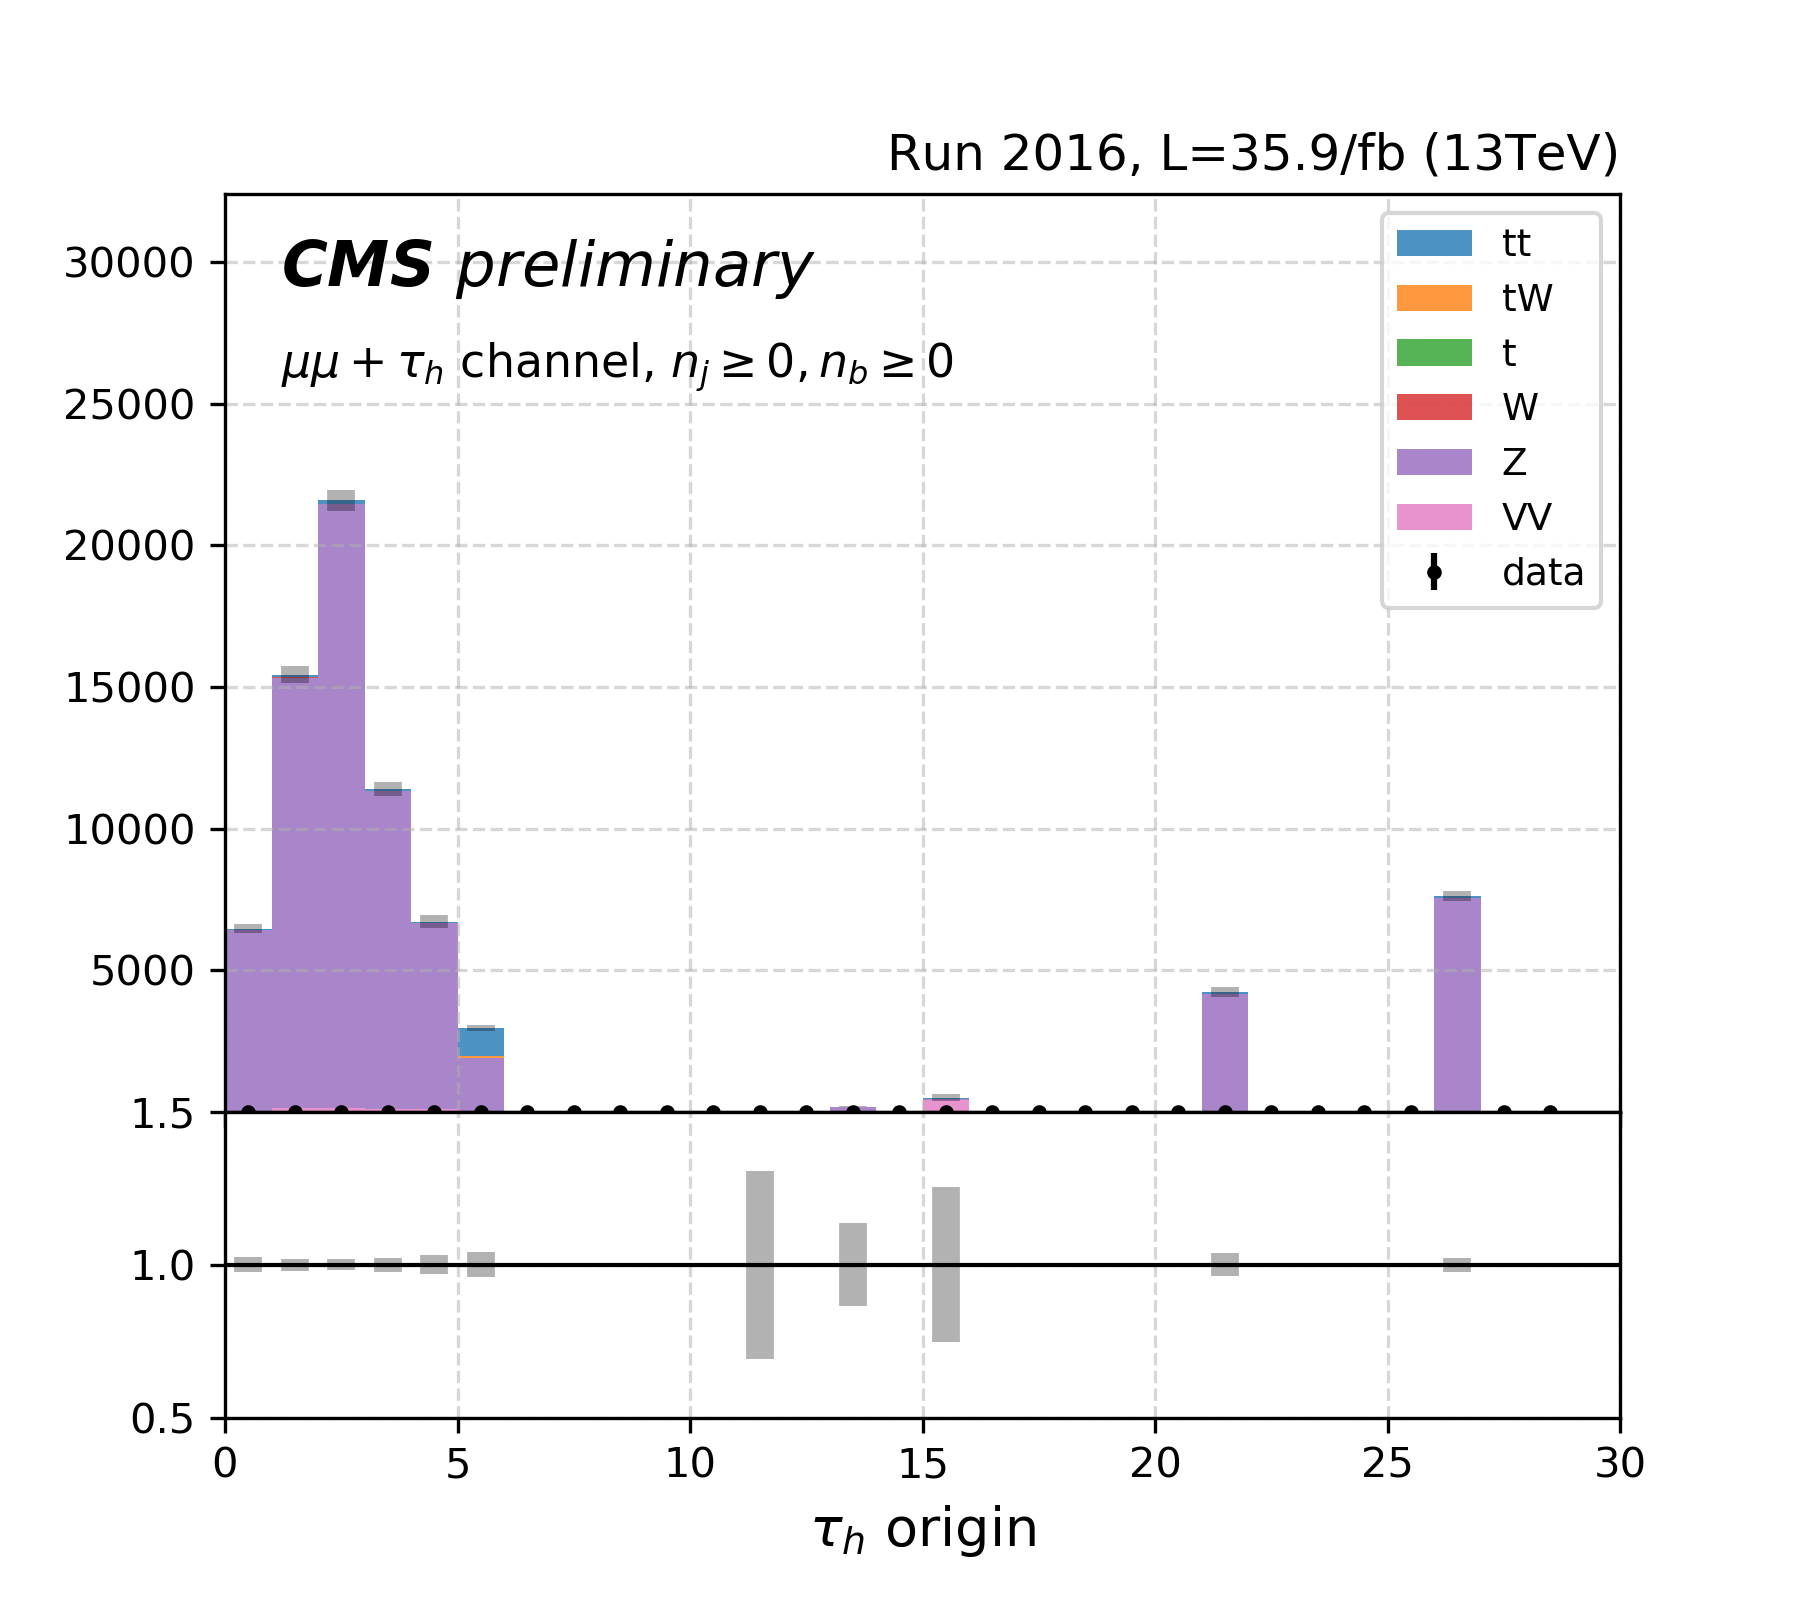
\includegraphics[width=0.4\textwidth]{appendices/jetToTauhReweighting/figures/mumutau_tauGenFlavor_pickles_lltauTight.png}
    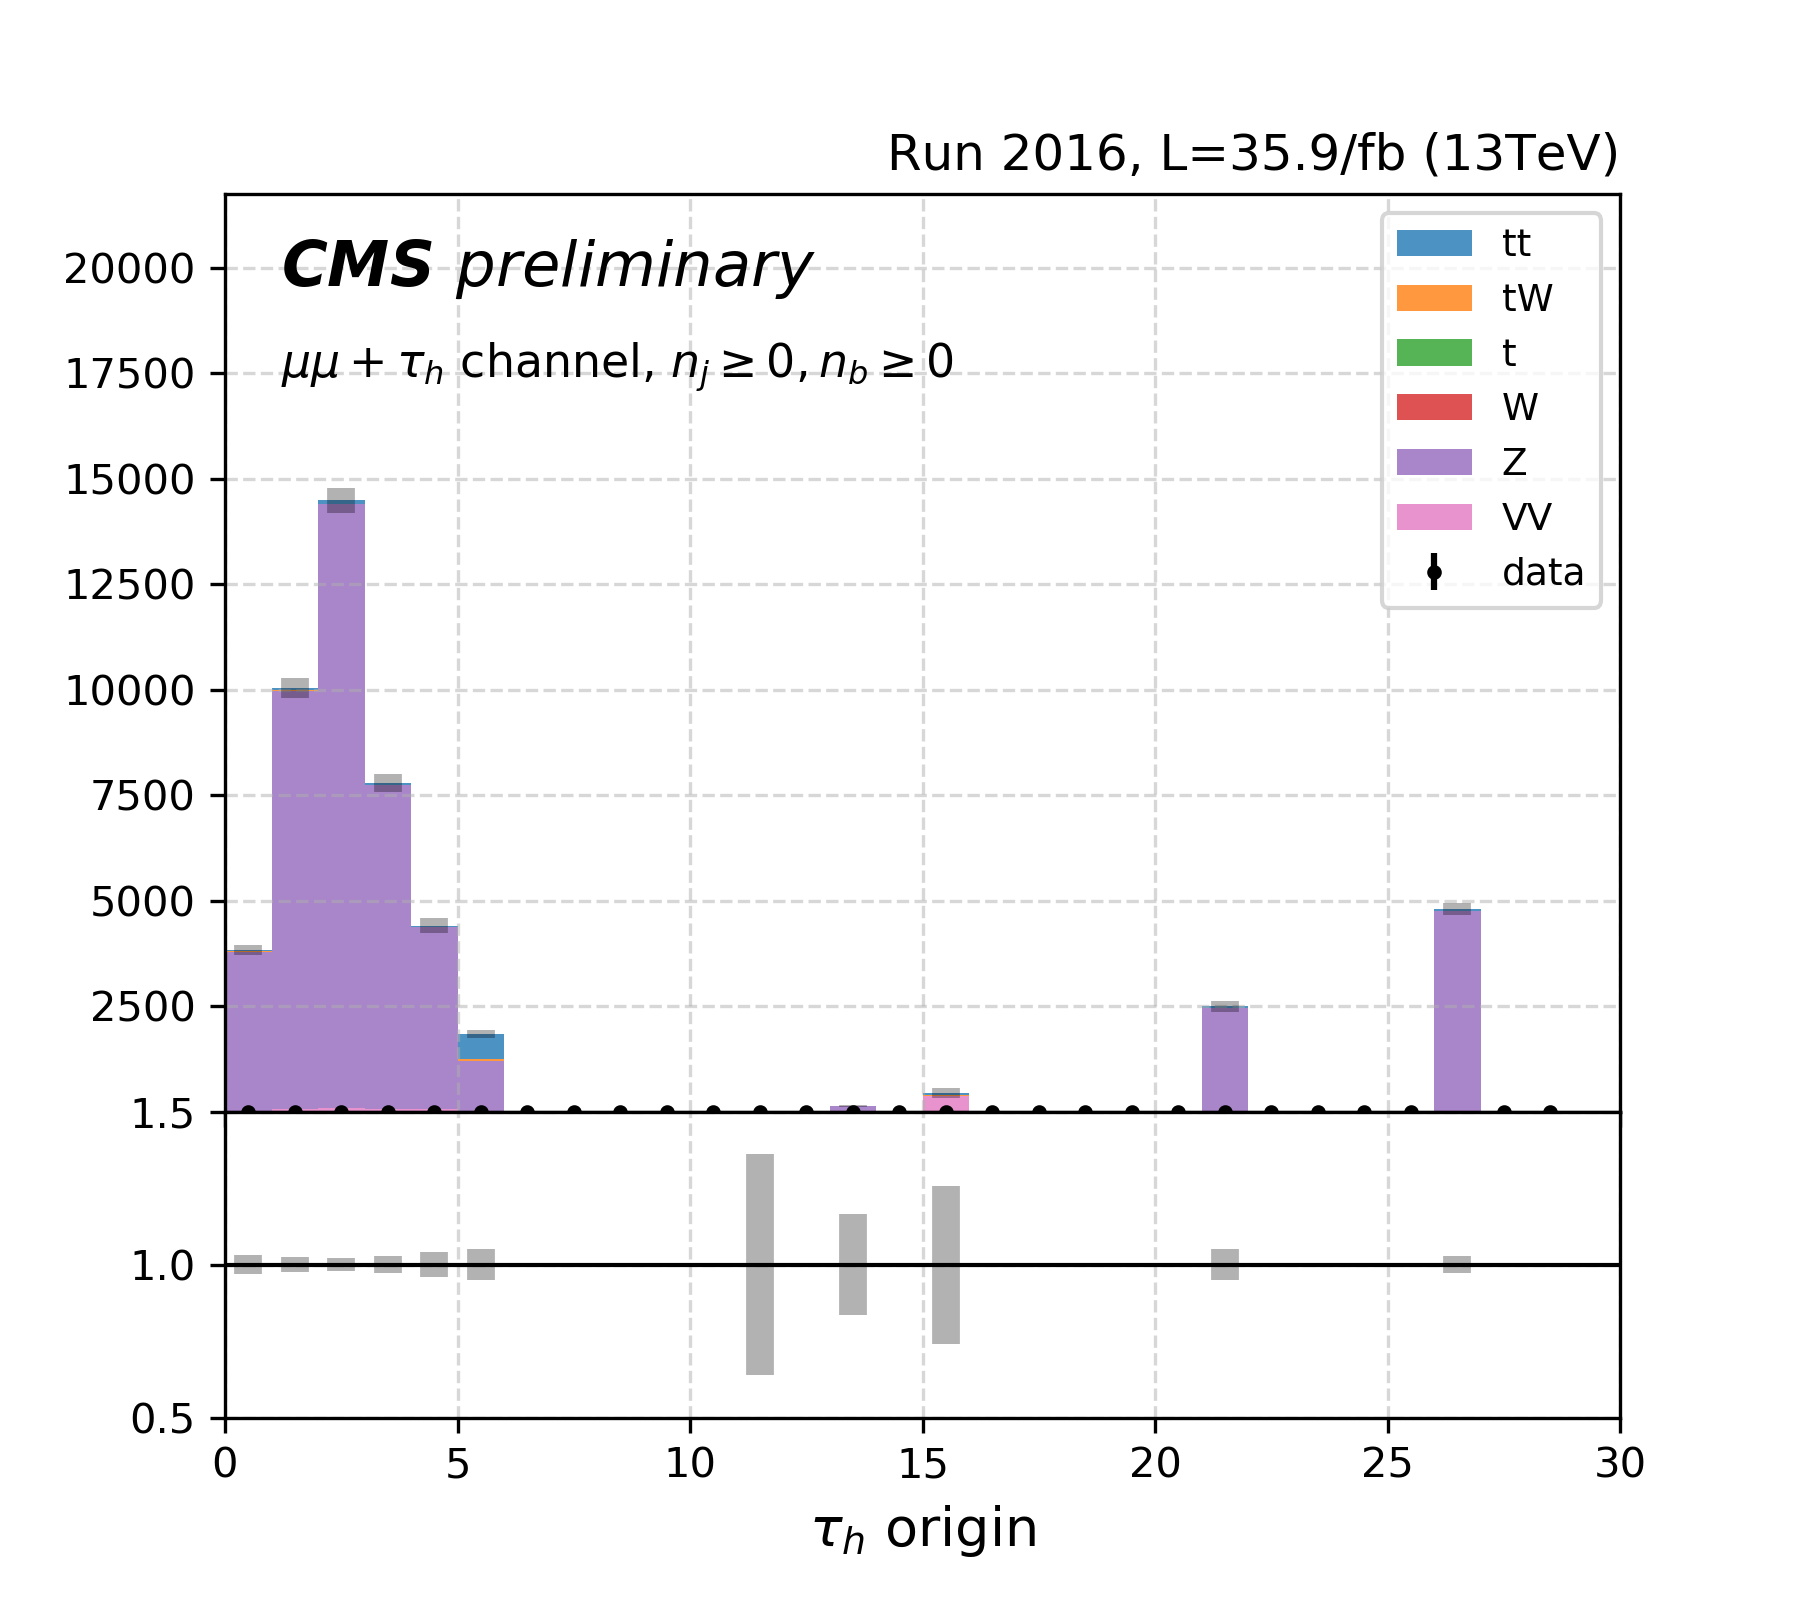
\includegraphics[width=0.4\textwidth]{appendices/jetToTauhReweighting/figures/mumutau_tauGenFlavor_pickles_lltauVTight.png}
    \caption{Distributions of $m_{\mu\mu}$, $\tau pT$ and gen-level $\tau_h$ origin in the $\mu\mu+\tau$ channel. The left and right column shows the Tight and VTight $\tau_h$ WP respectively.}
    \label{fig:appendix:fakeTauId:mumutau}
\end{figure}


\begin{figure}
    \centering
    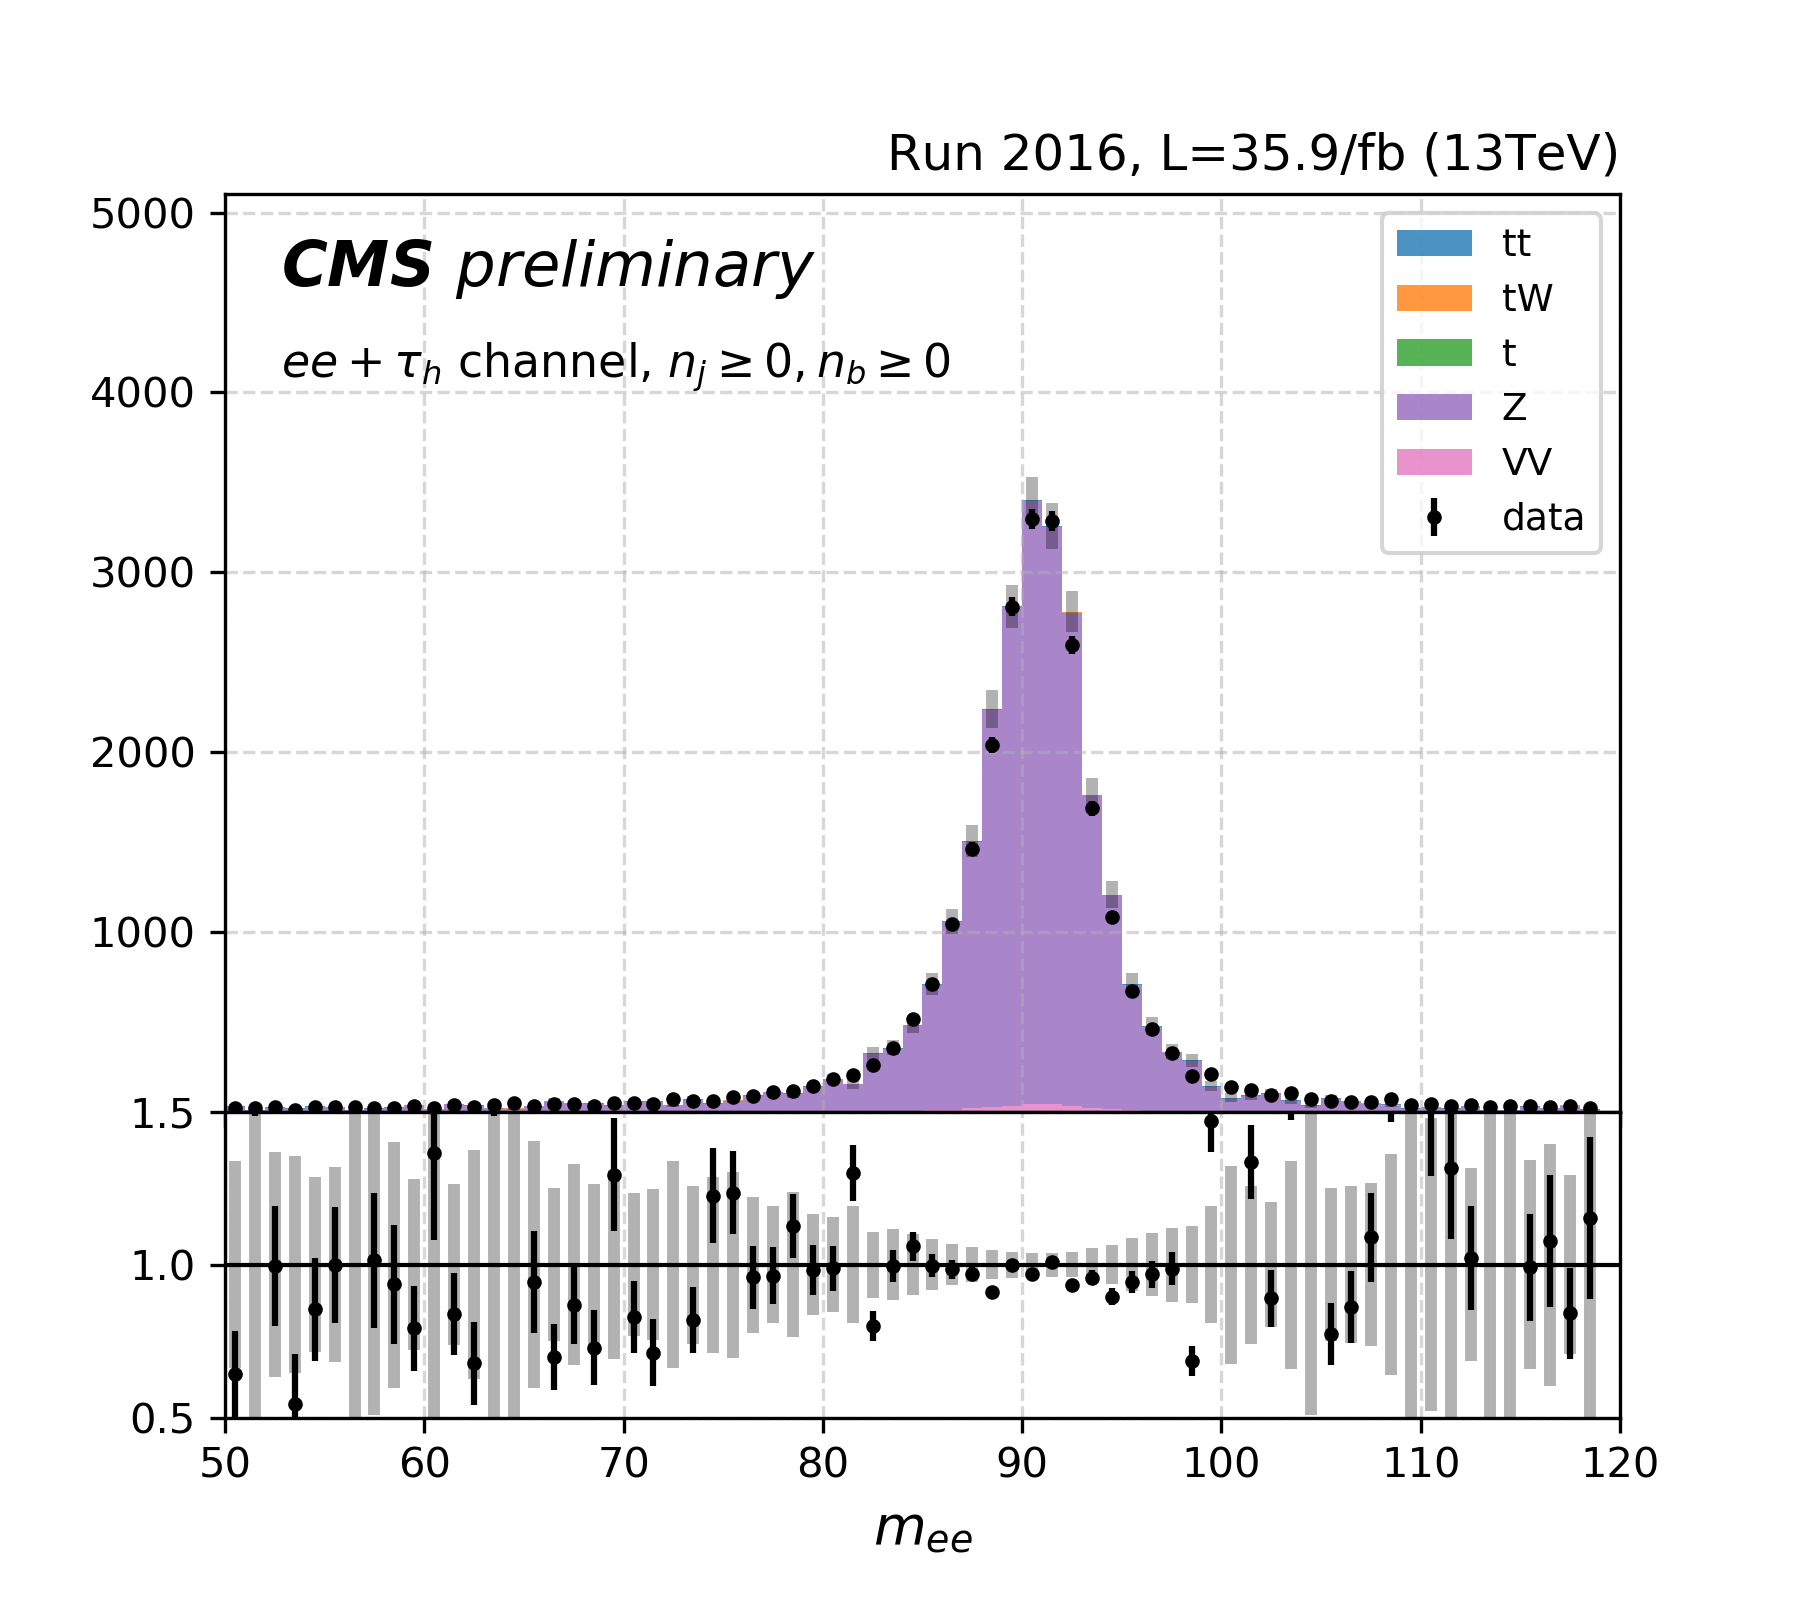
\includegraphics[width=0.4\textwidth]{appendices/jetToTauhReweighting/figures/eetau_dilepton_mass_pickles_lltauTight.png}
    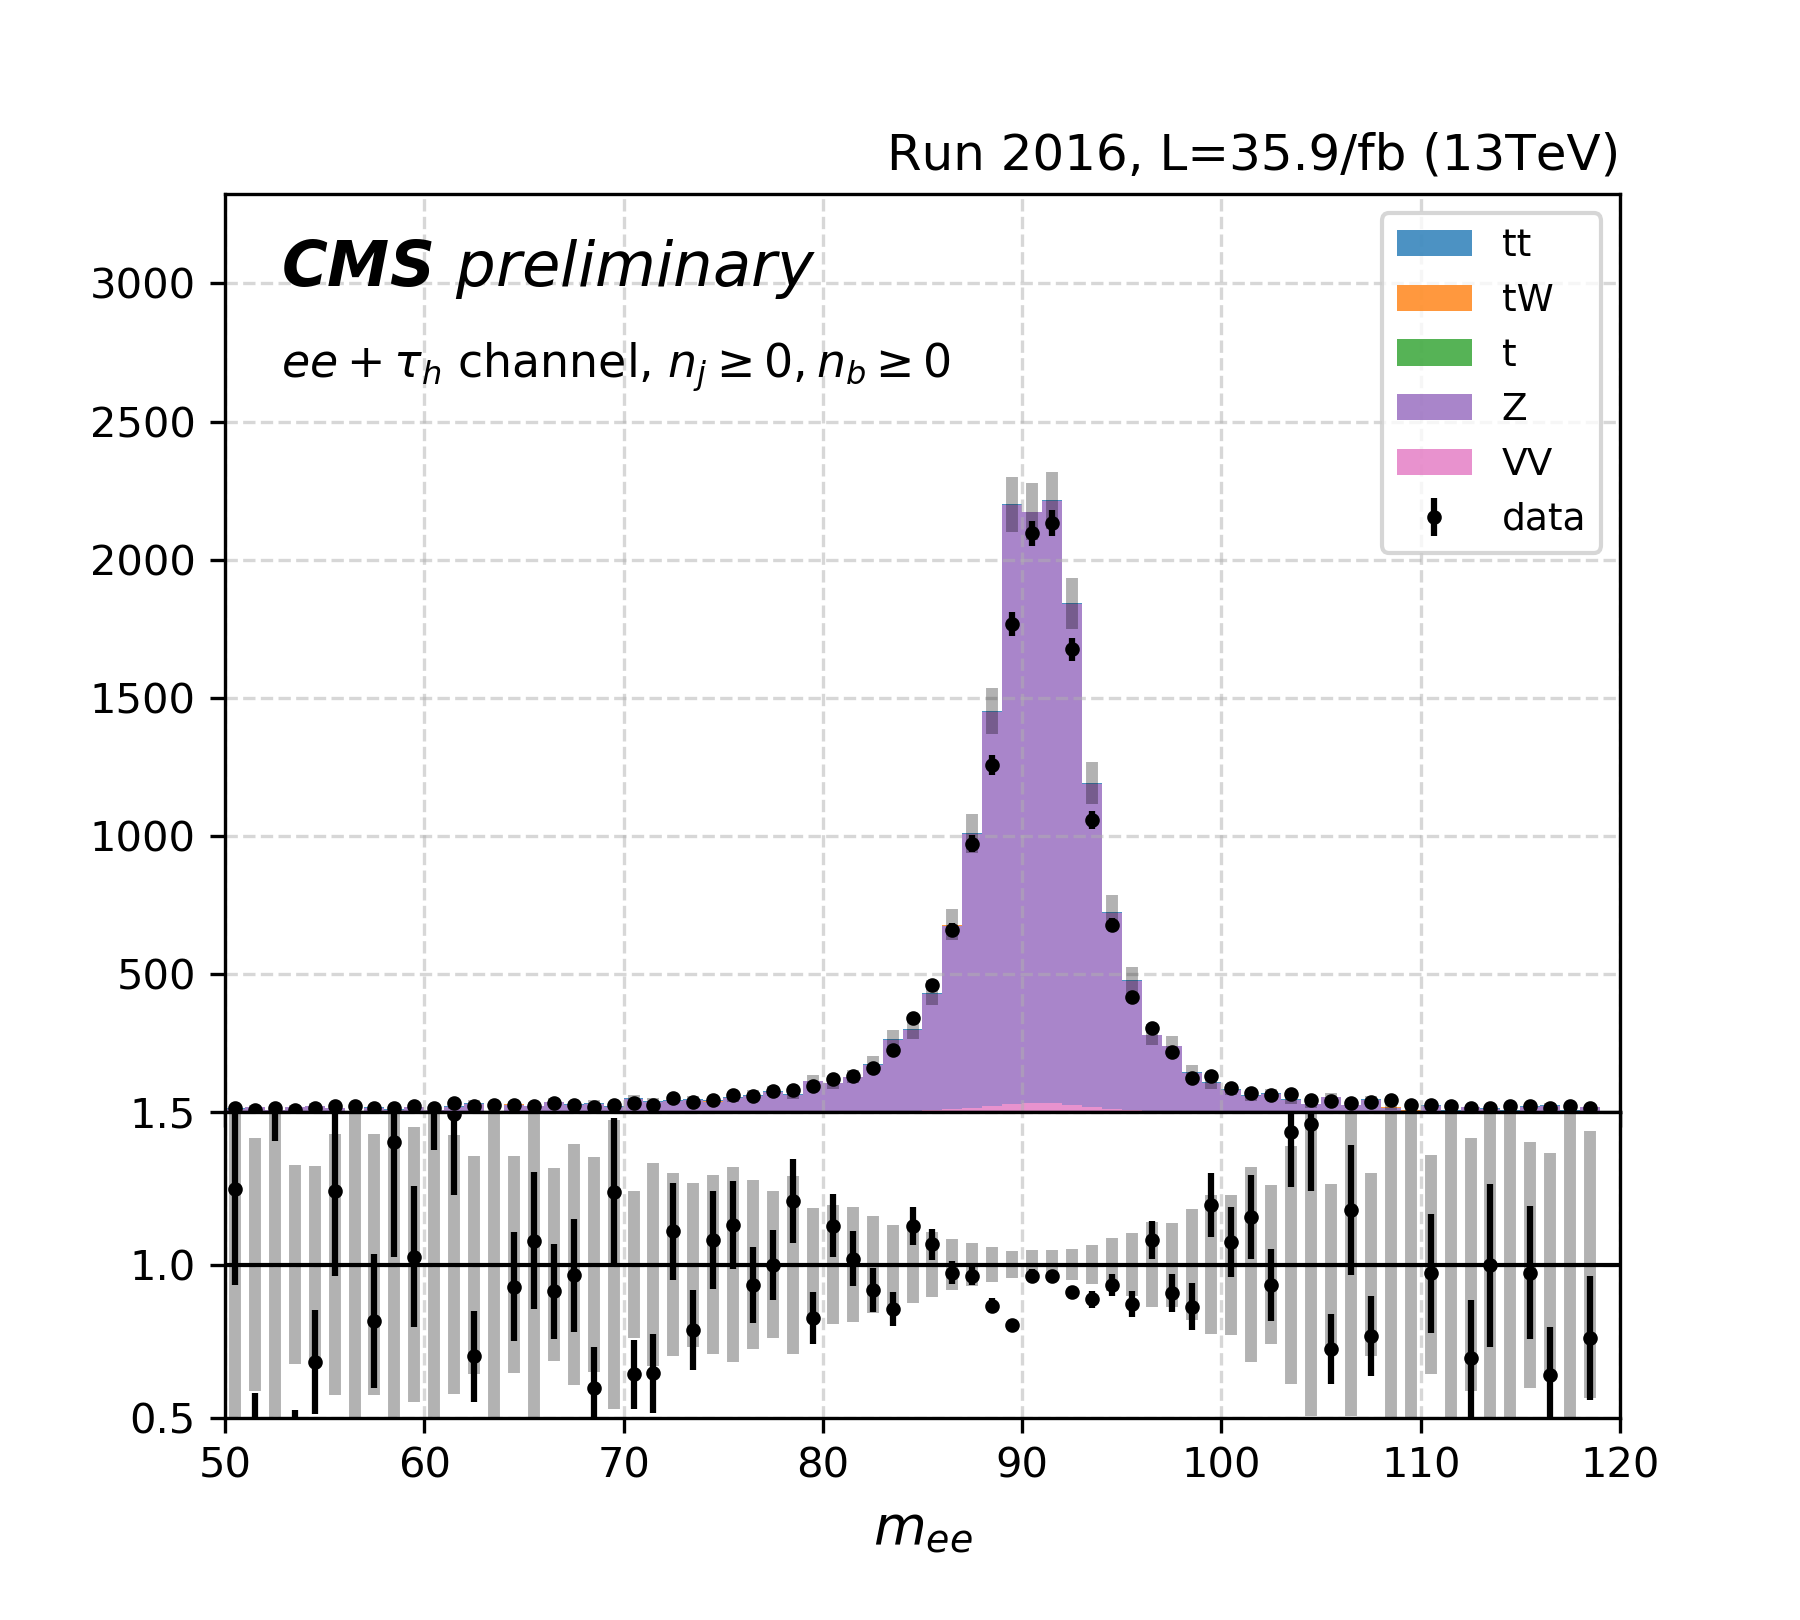
\includegraphics[width=0.4\textwidth]{appendices/jetToTauhReweighting/figures/eetau_dilepton_mass_pickles_lltauVTight.png}
    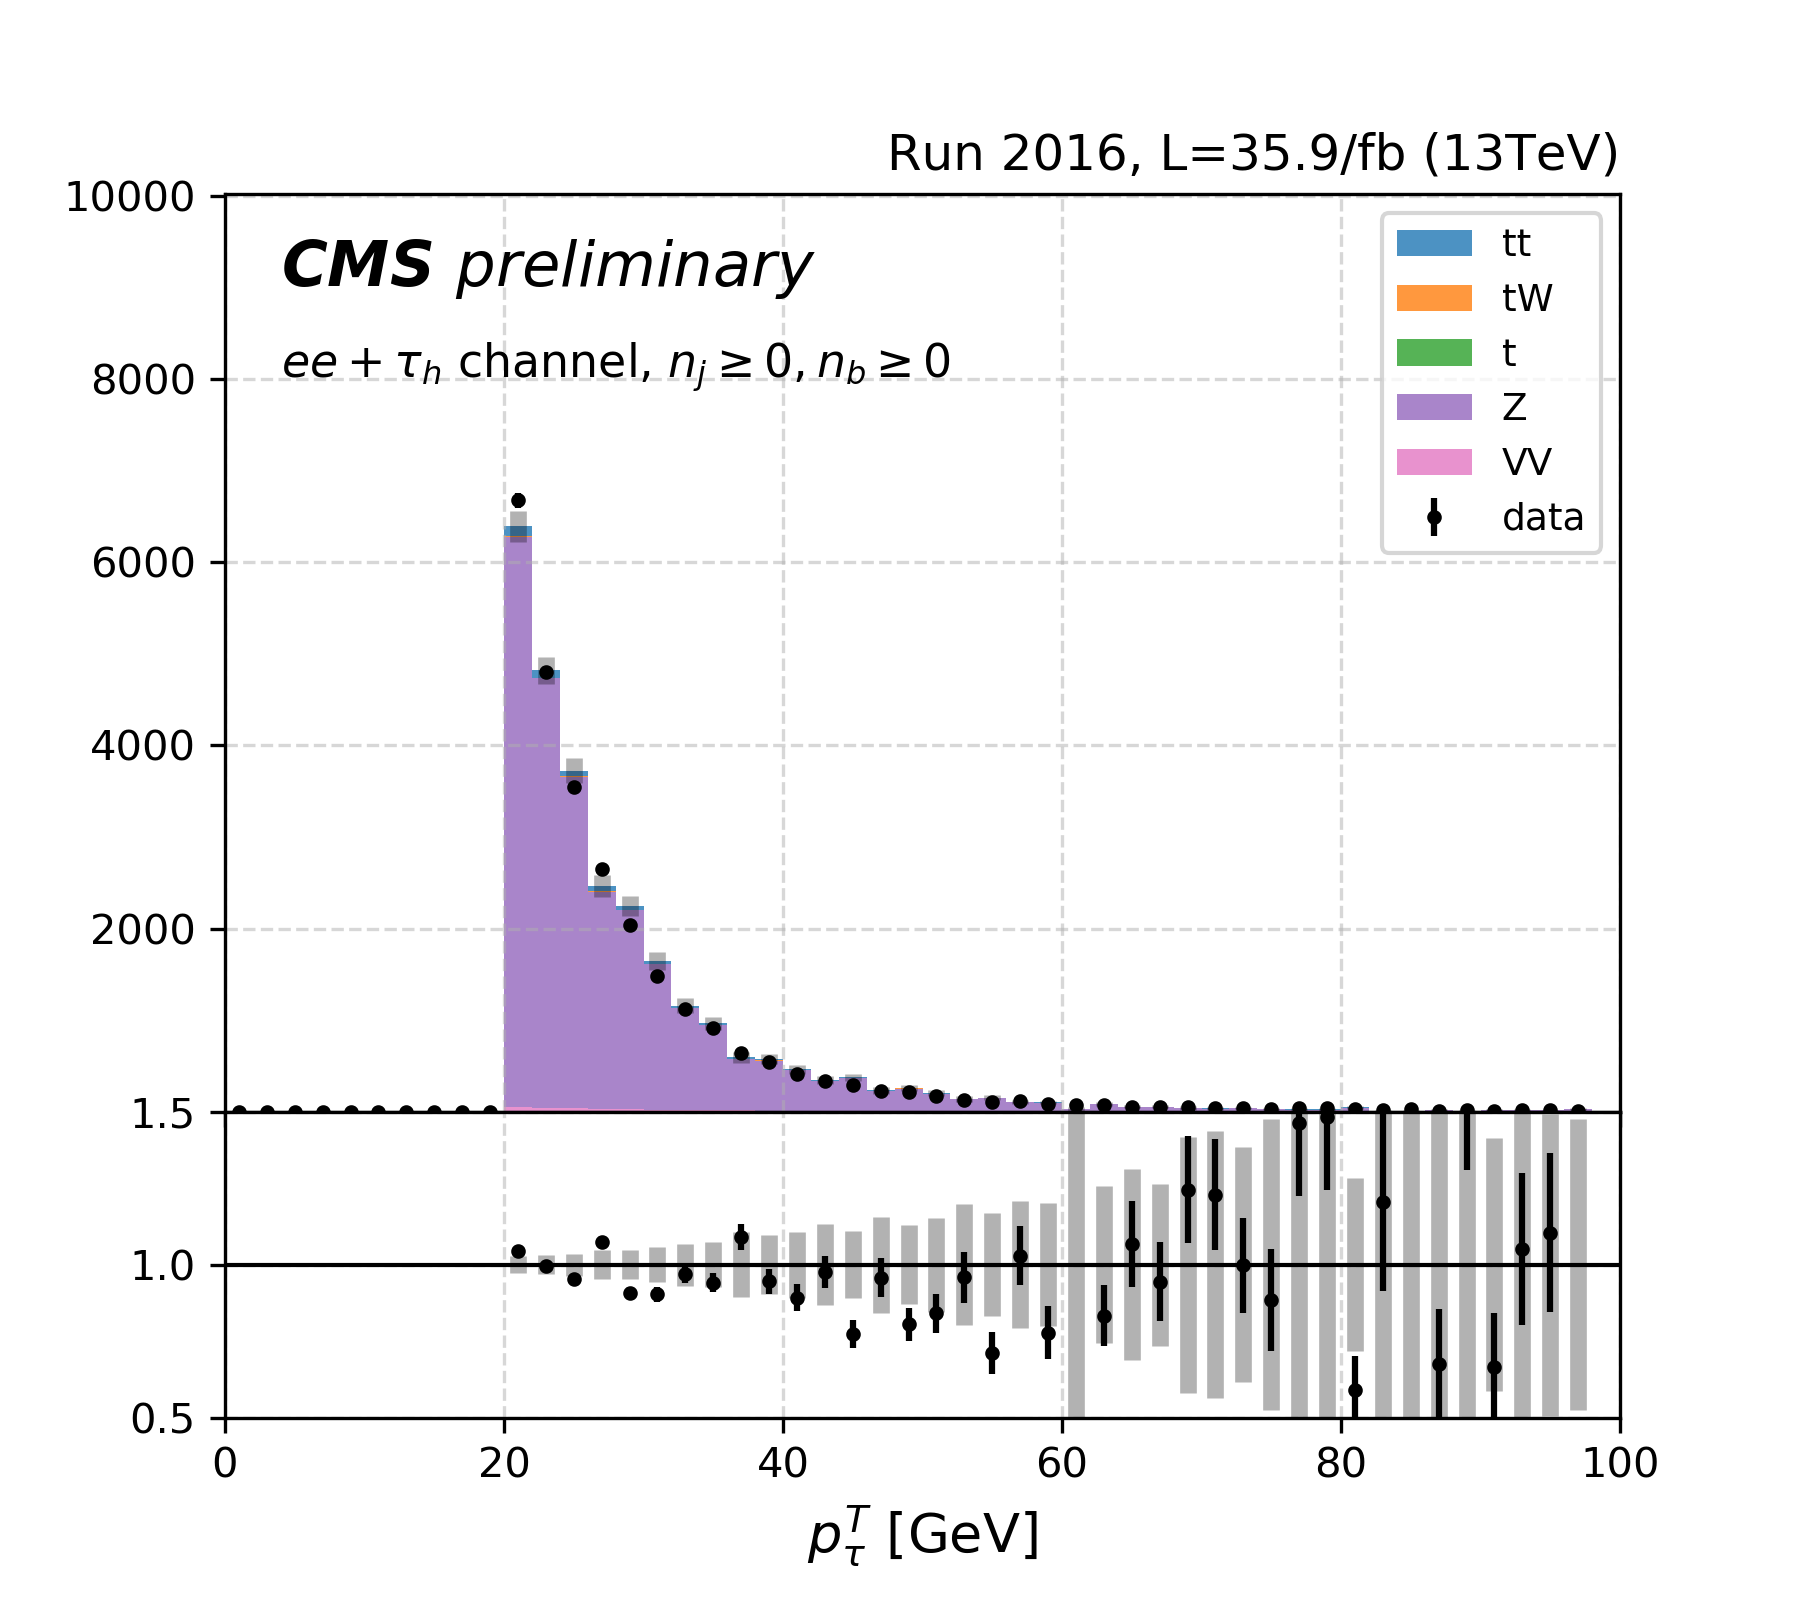
\includegraphics[width=0.4\textwidth]{appendices/jetToTauhReweighting/figures/eetau_tauPt_pickles_lltauTight.png}
    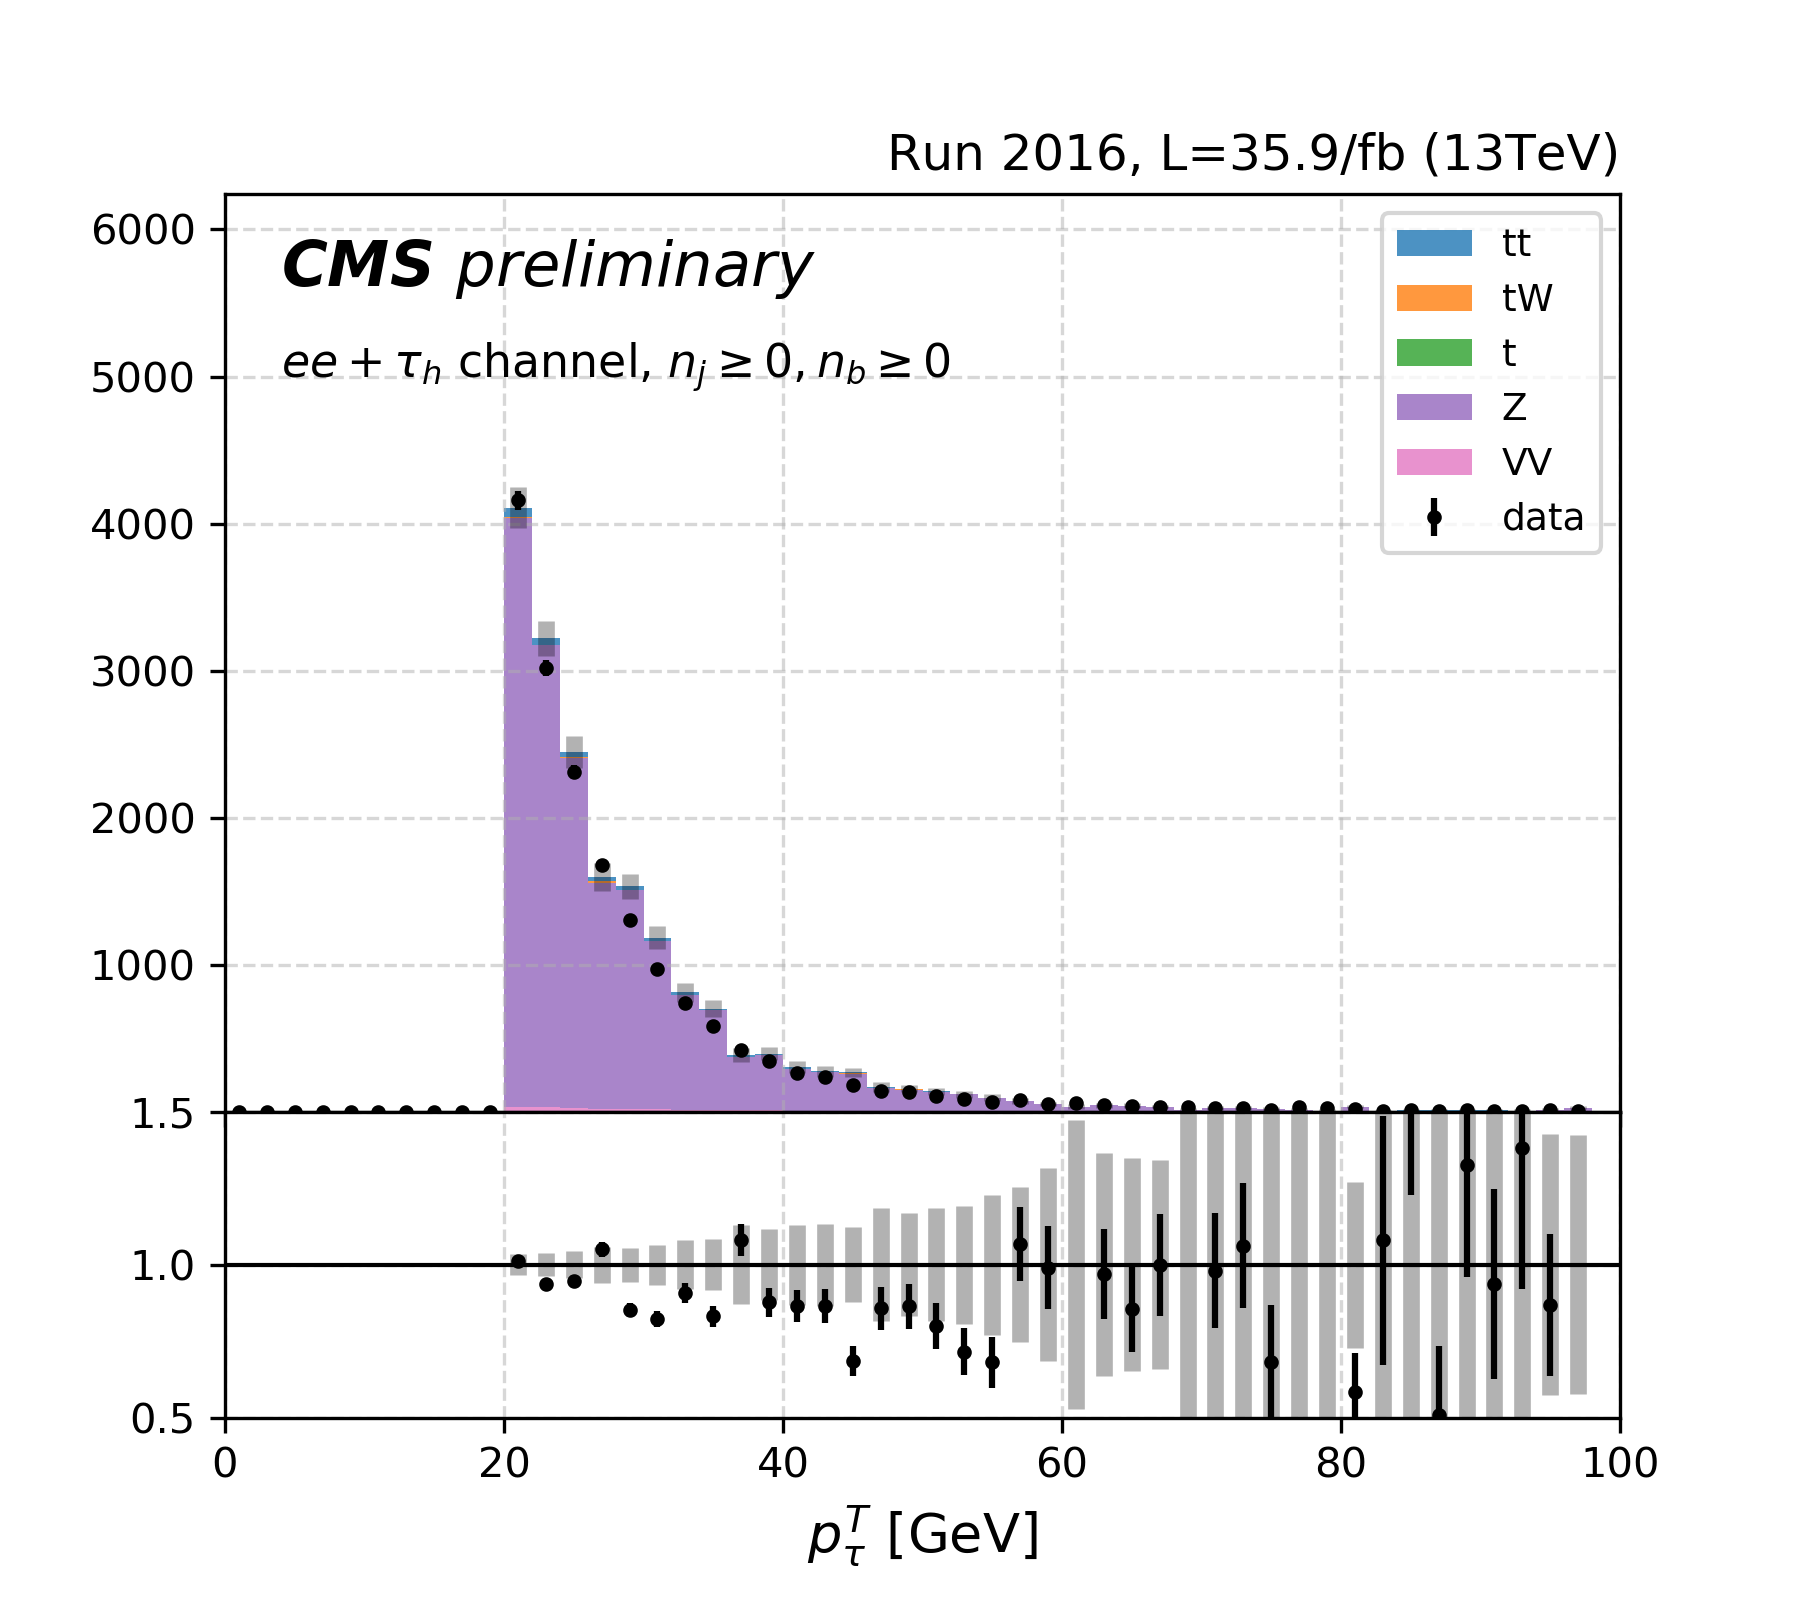
\includegraphics[width=0.4\textwidth]{appendices/jetToTauhReweighting/figures/eetau_tauPt_pickles_lltauVTight.png}
    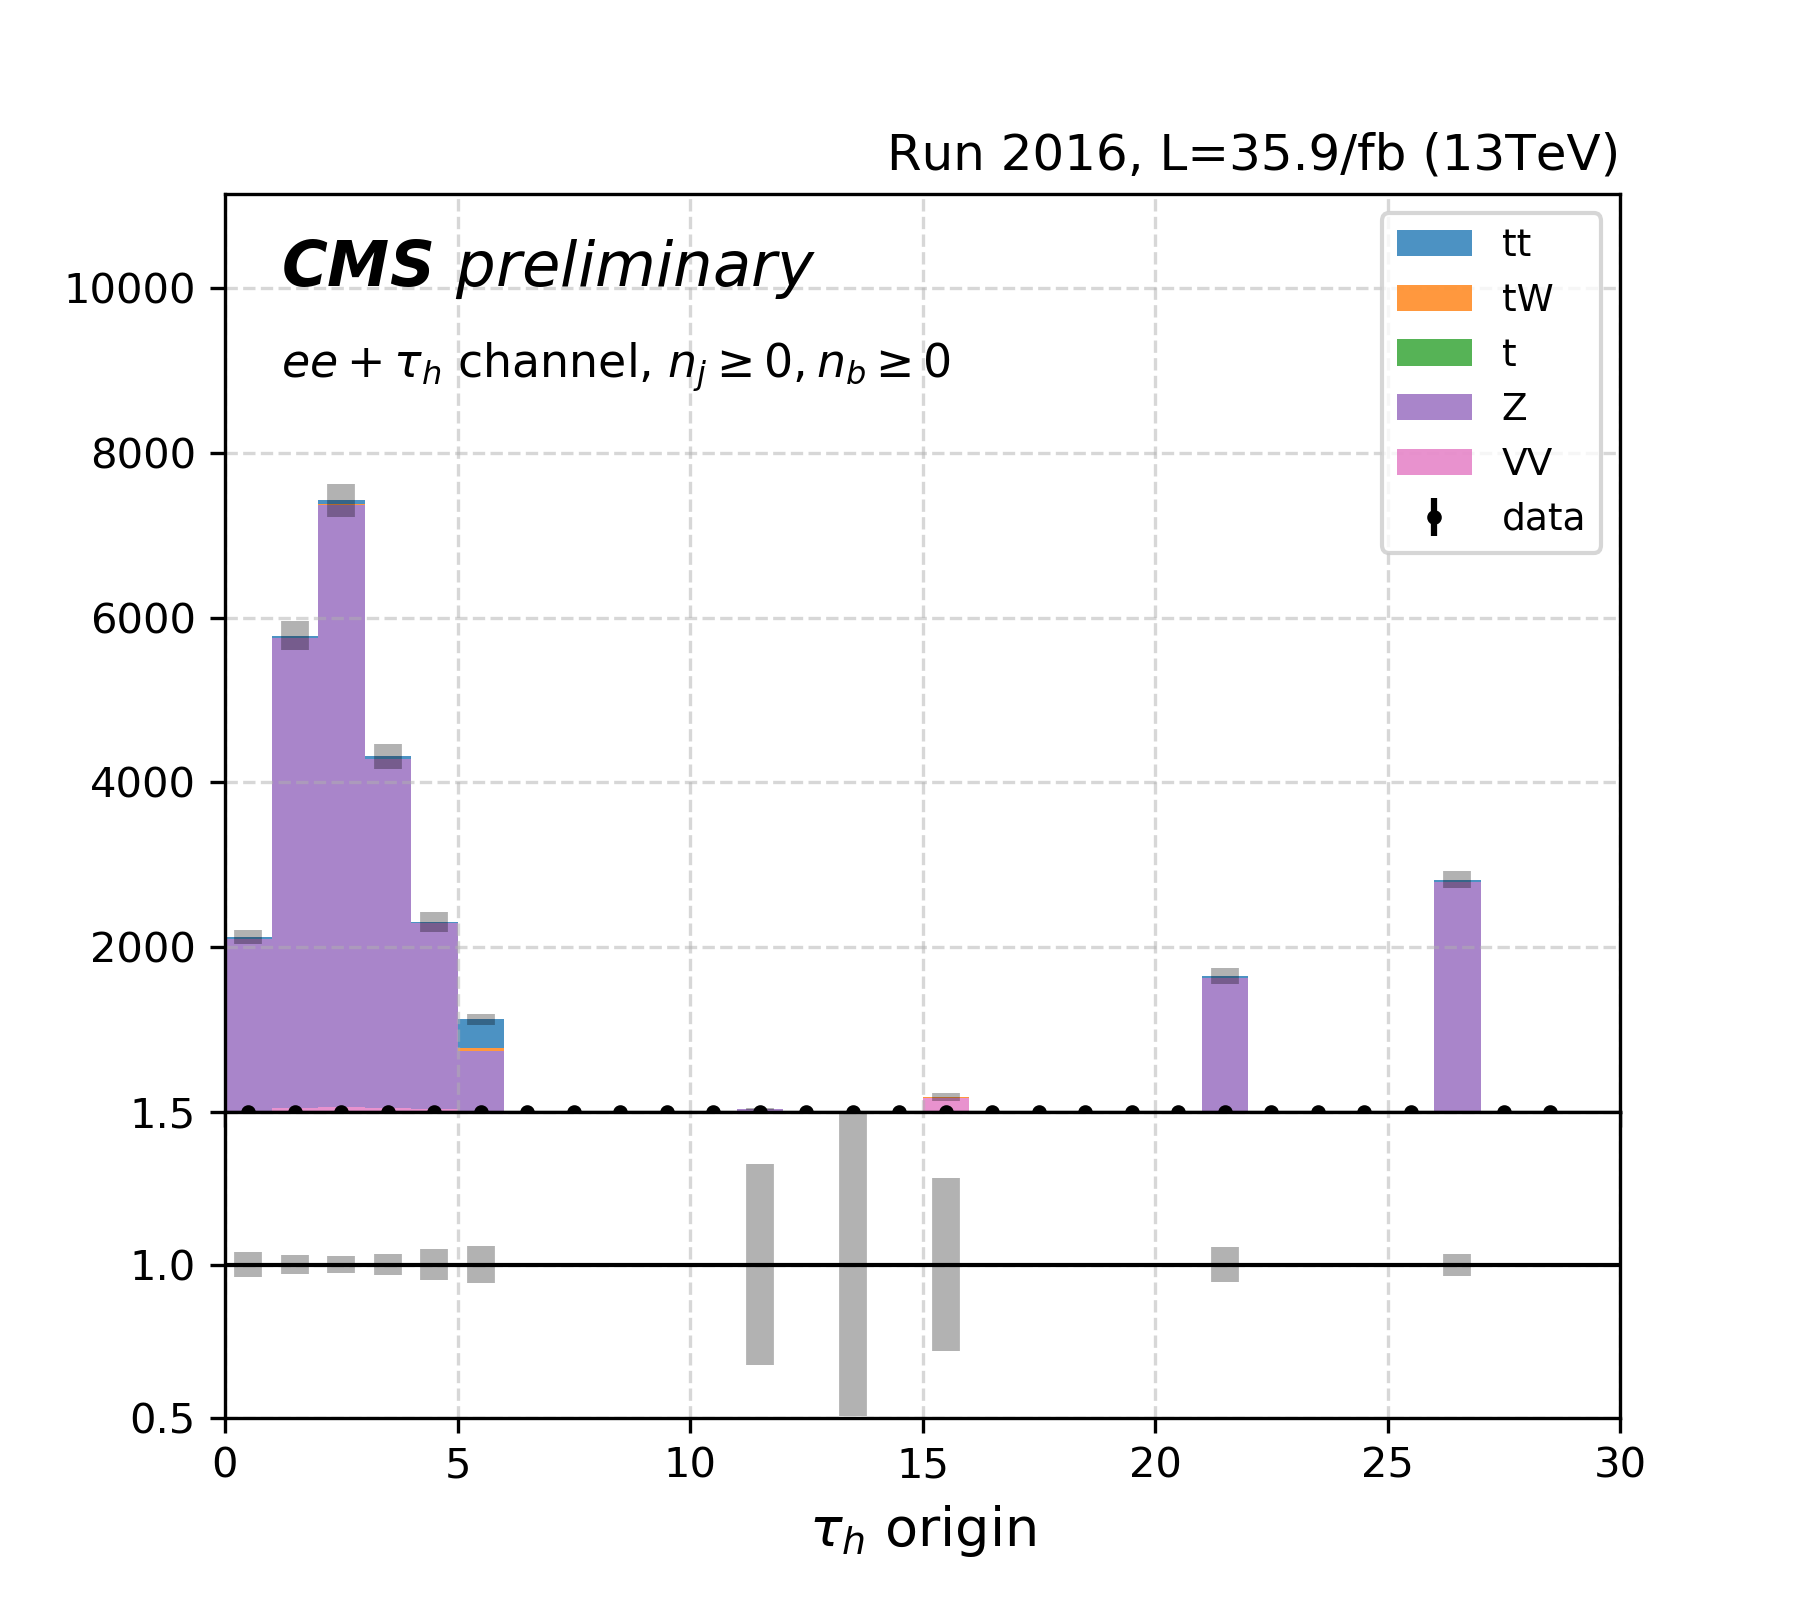
\includegraphics[width=0.4\textwidth]{appendices/jetToTauhReweighting/figures/eetau_tauGenFlavor_pickles_lltauTight.png}
    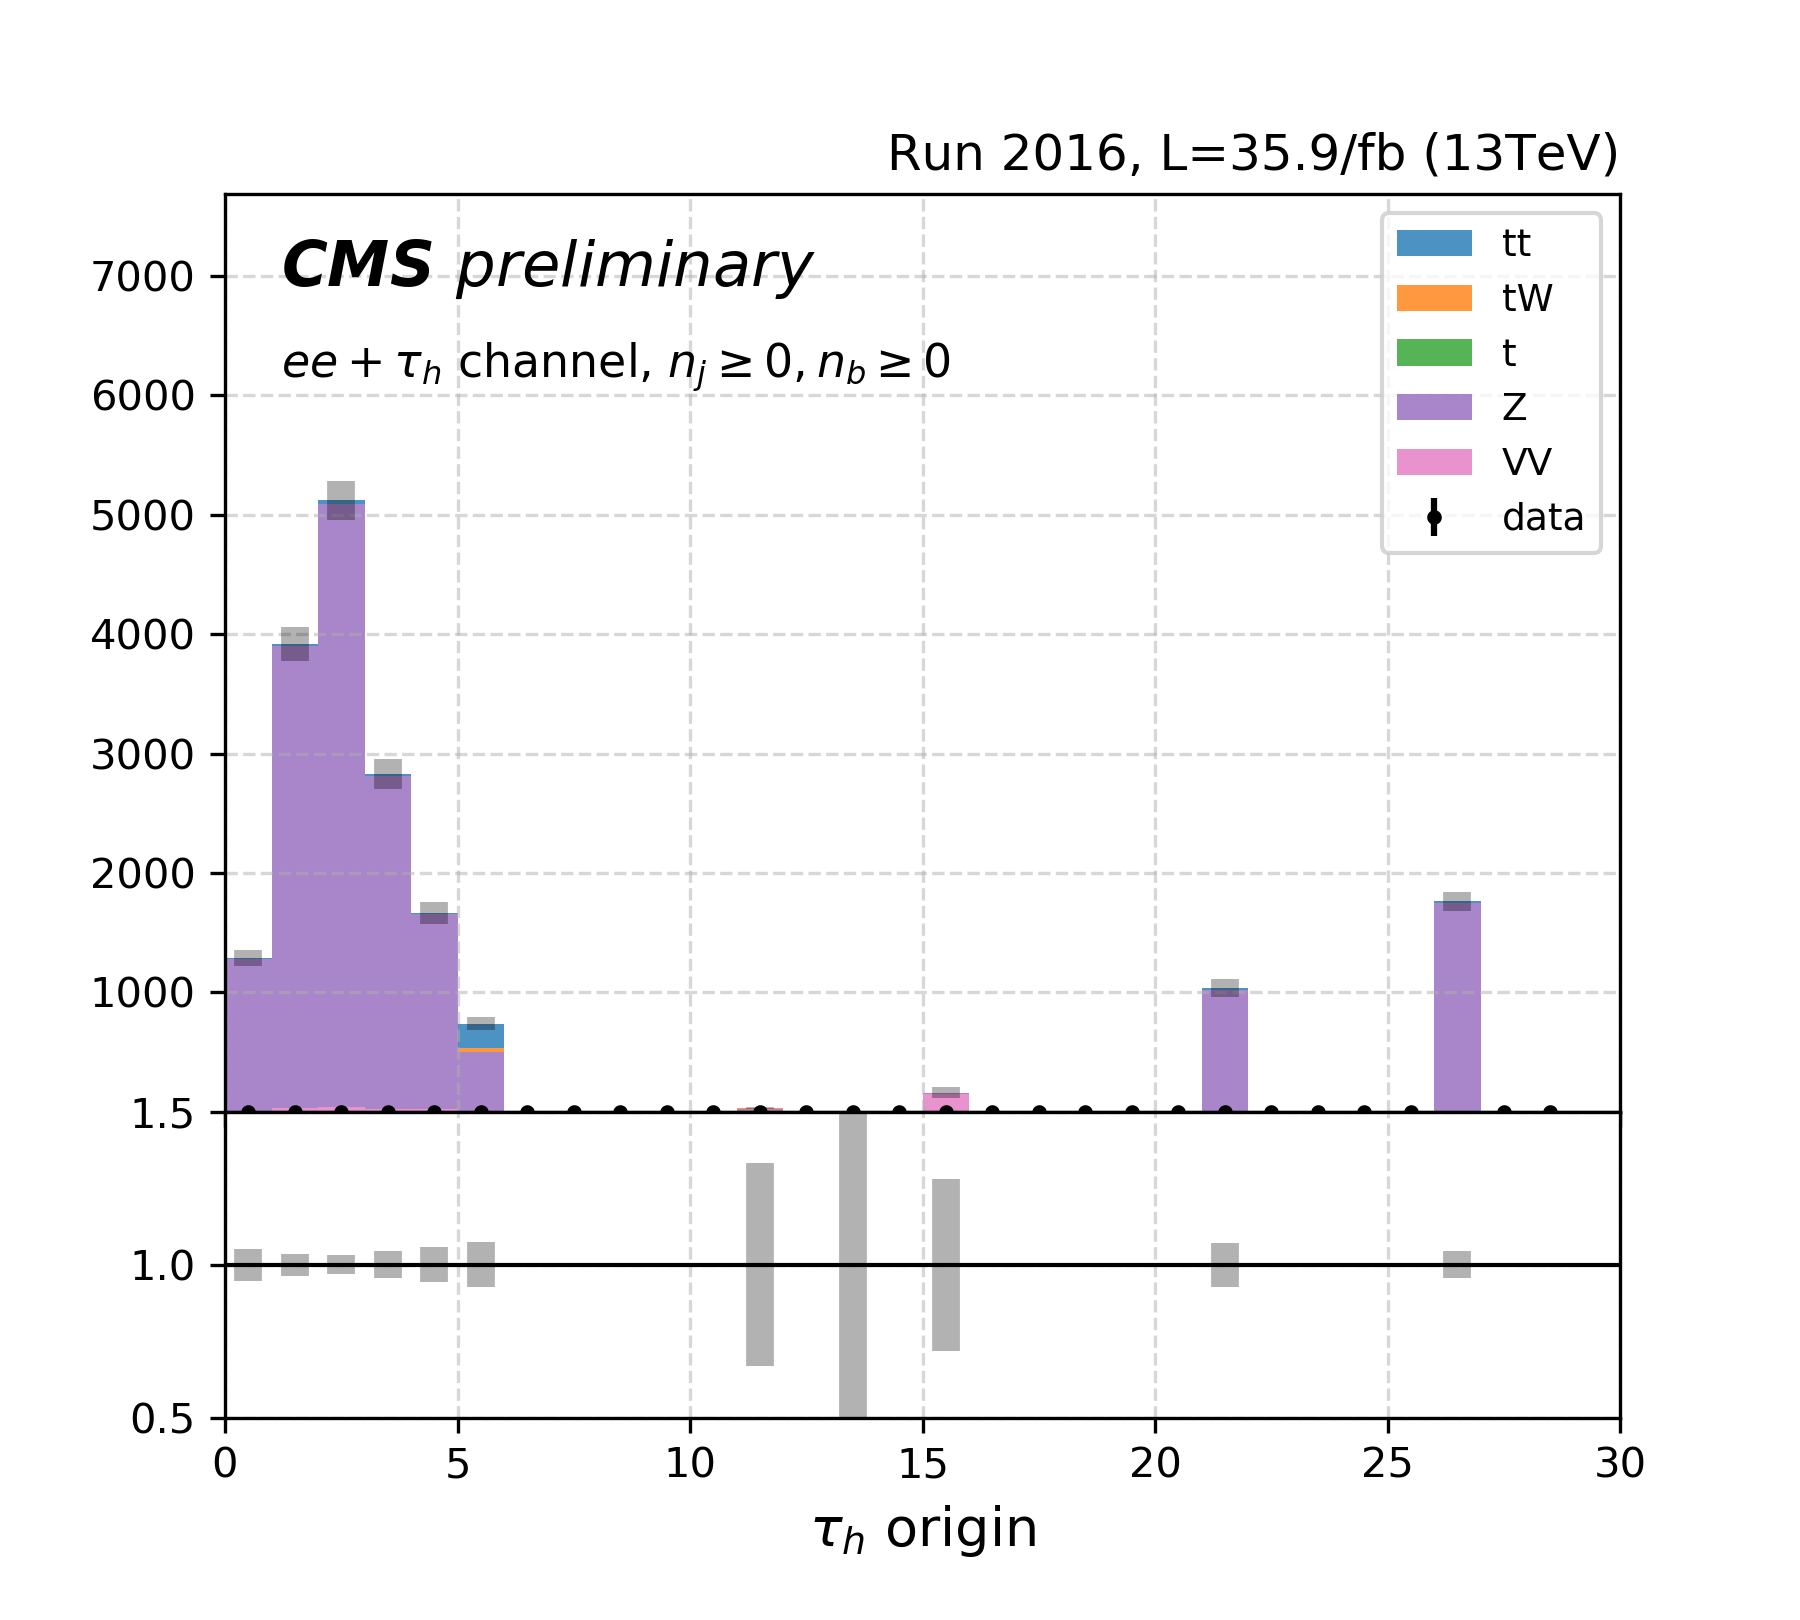
\includegraphics[width=0.4\textwidth]{appendices/jetToTauhReweighting/figures/eetau_tauGenFlavor_pickles_lltauVTight.png}
    \caption{Distributions of $m_{ee}$, $\tau pT$ and gen-level $\tau_h$ origin in the $ee+\tau$ channel. The left and right column shows the Tight and VTight $\tau_h$ WP respectively.}
    \label{fig:appendix:fakeTauId:eetau}
\end{figure}


\begin{figure}
    \centering
    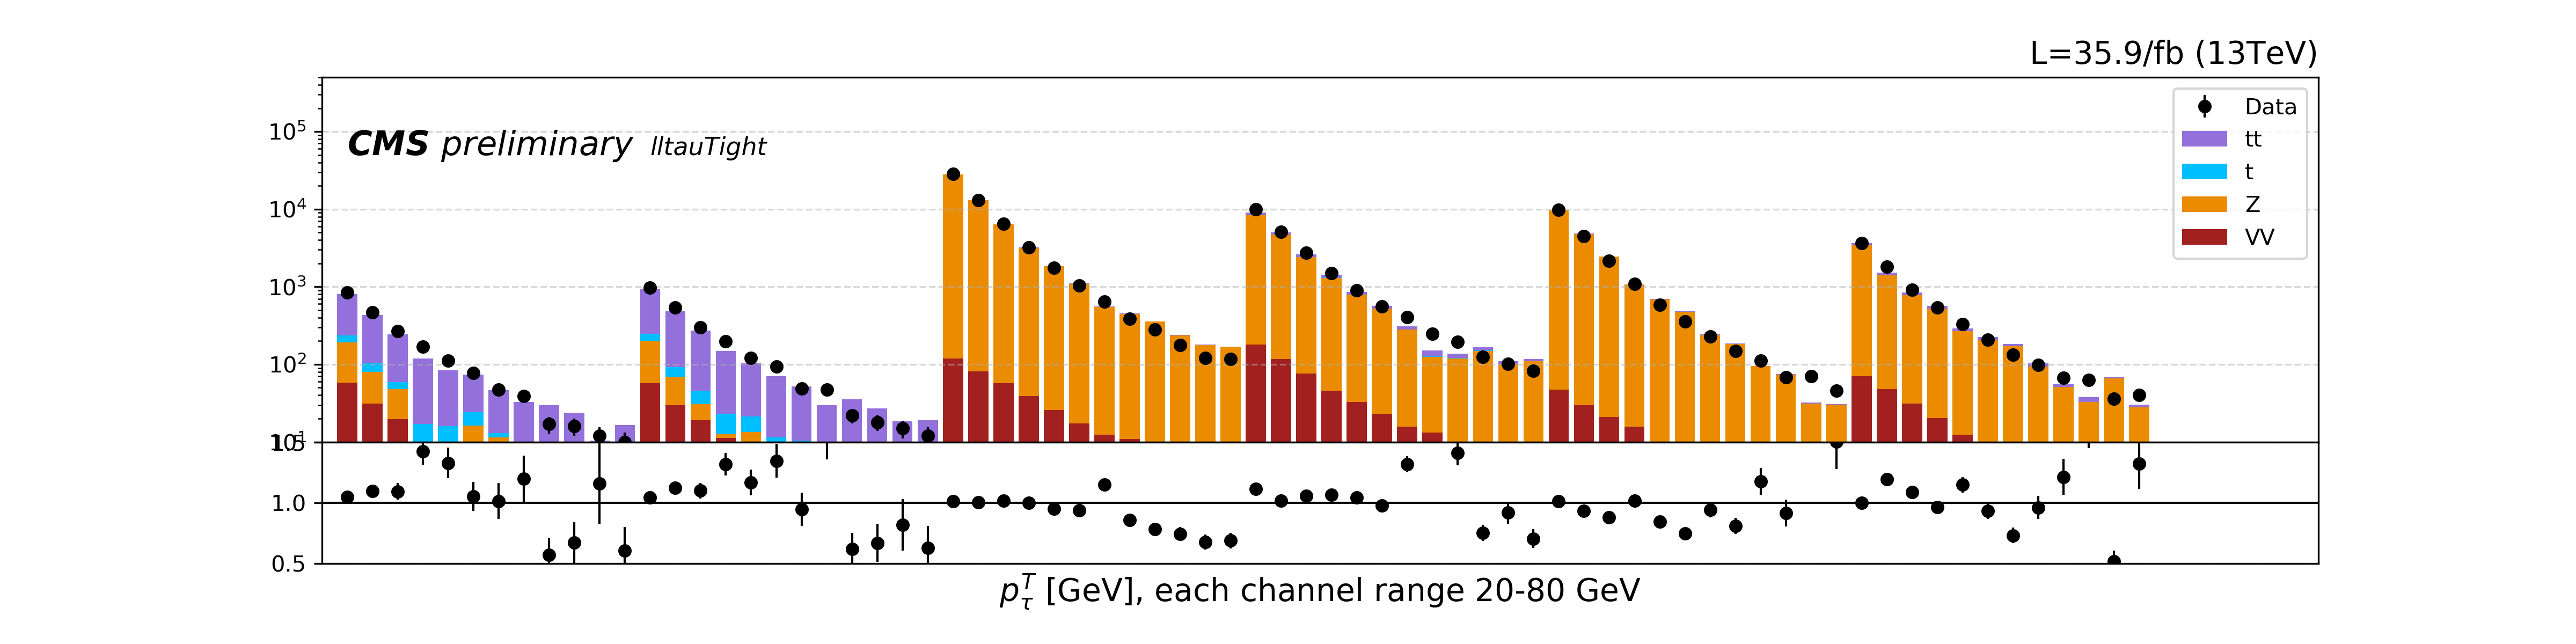
\includegraphics[width=0.99\textwidth]{appendices/jetToTauhReweighting/figures/2020_tauID_prefit_lltauTight.png}
    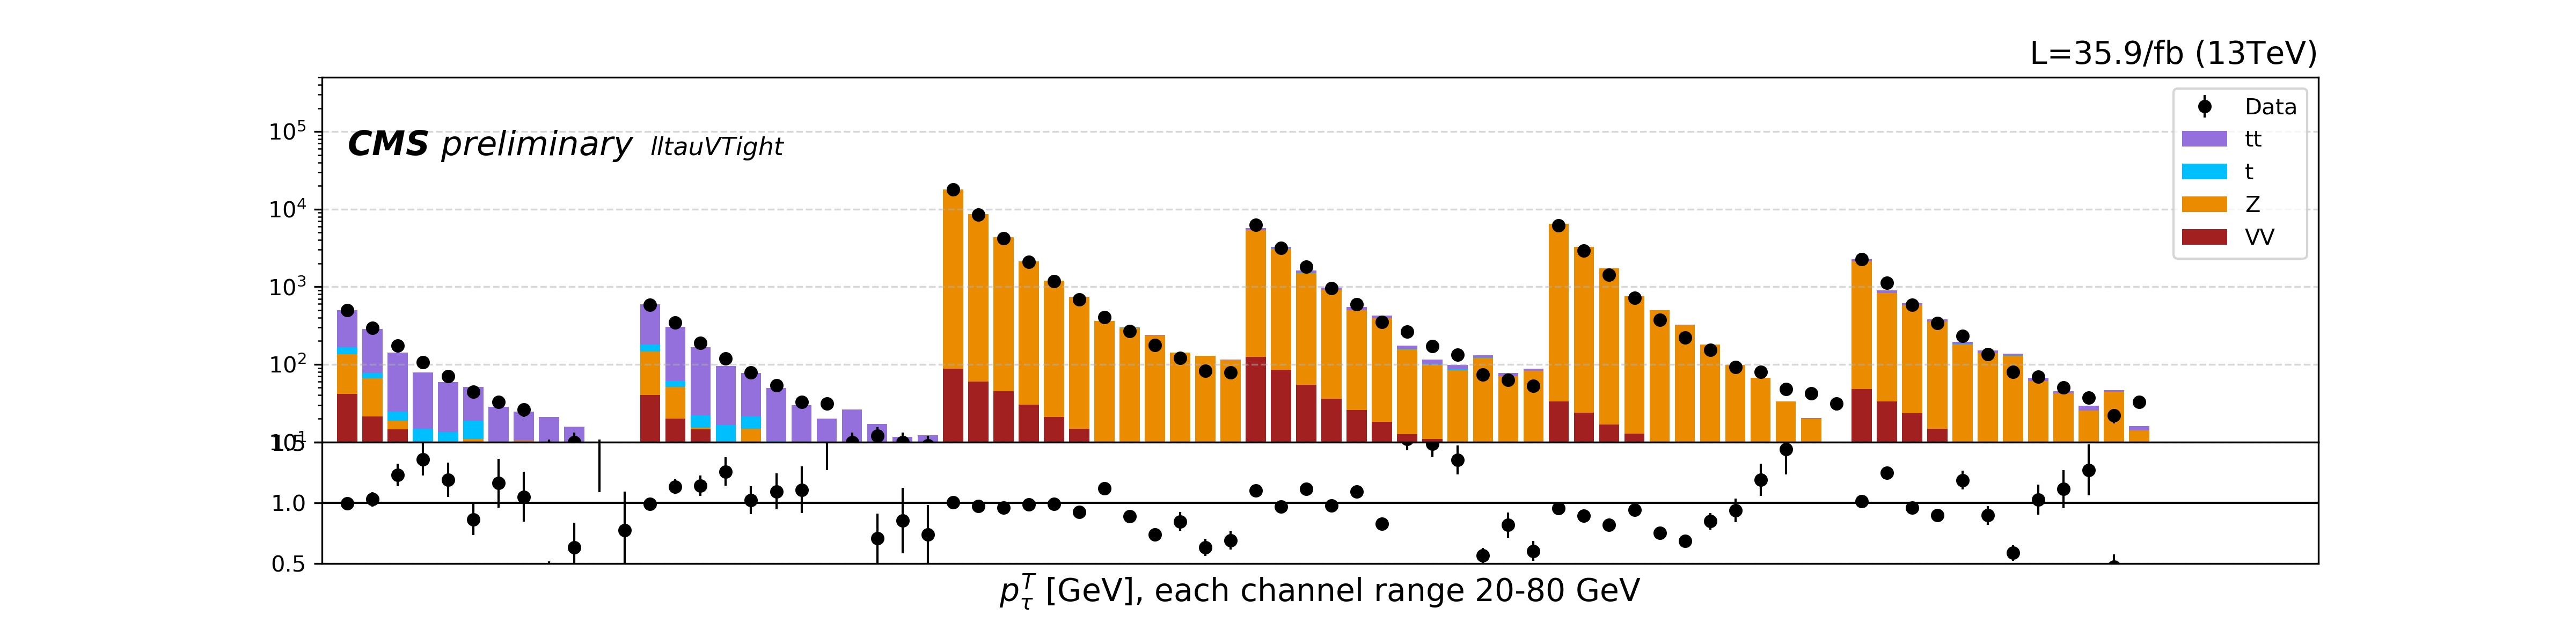
\includegraphics[width=0.99\textwidth]{appendices/jetToTauhReweighting/figures/2020_tauID_prefit_lltauVTight.png}
    \caption{Prefit distributions}
    \label{fig:appendix:fakeTauId:prefit}
\end{figure}

\begin{figure}
    \centering
    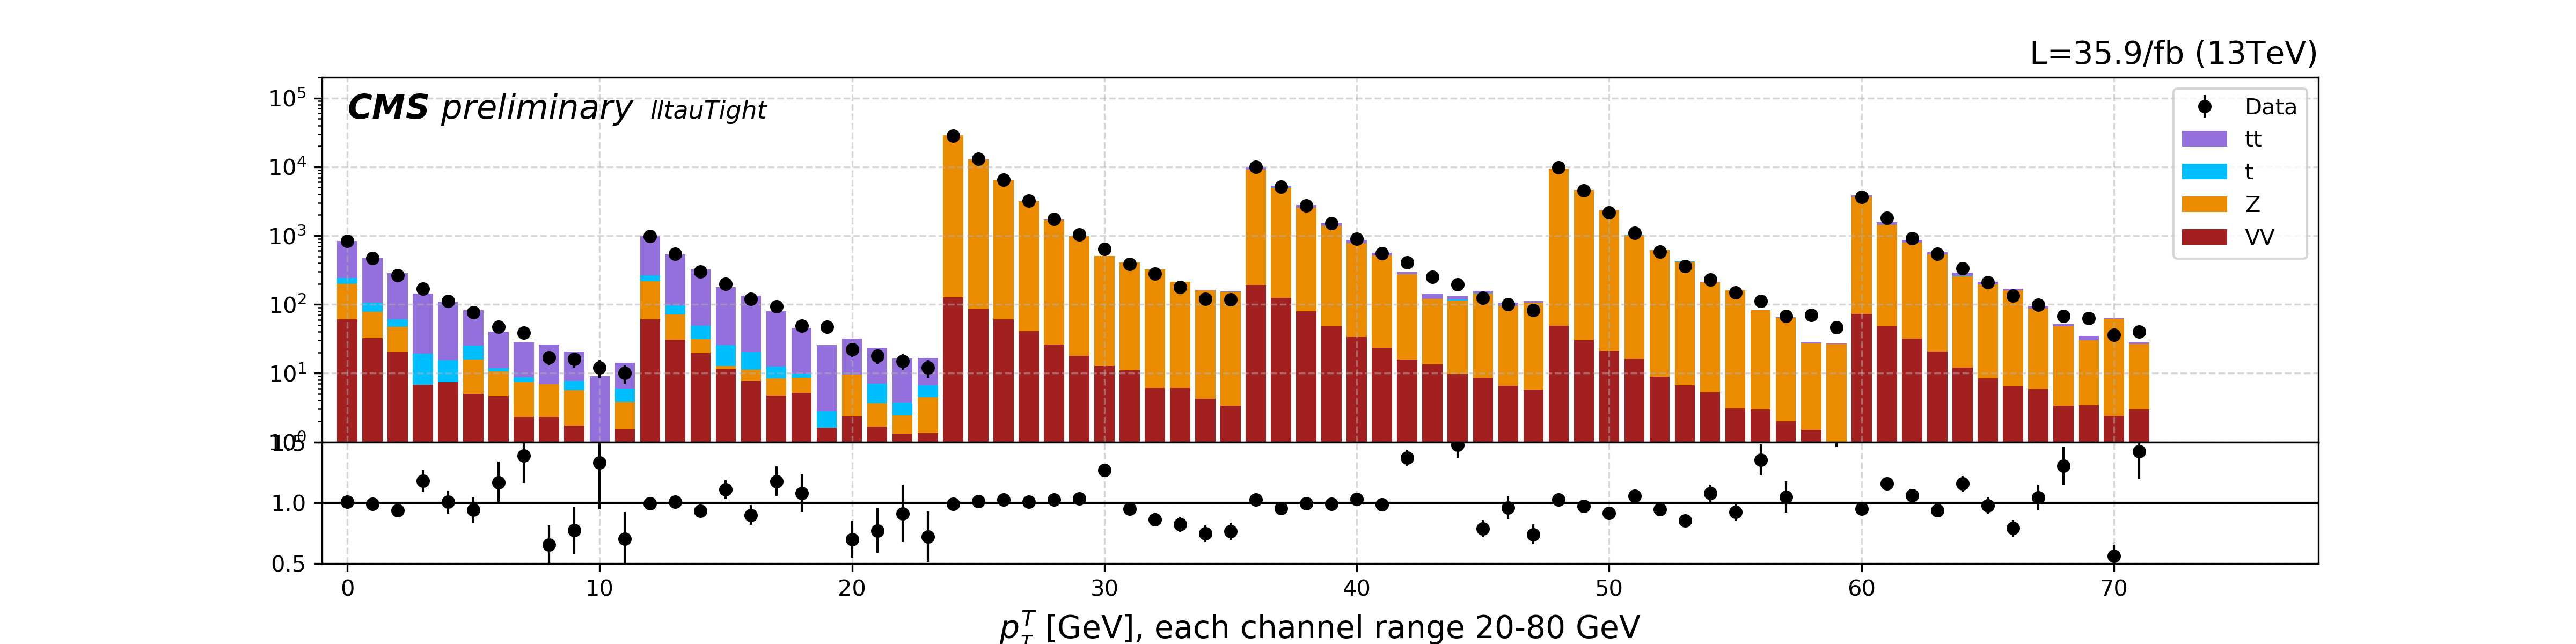
\includegraphics[width=0.99\textwidth]{appendices/jetToTauhReweighting/figures/2020_tauID_postfit_lltauTight.png}
    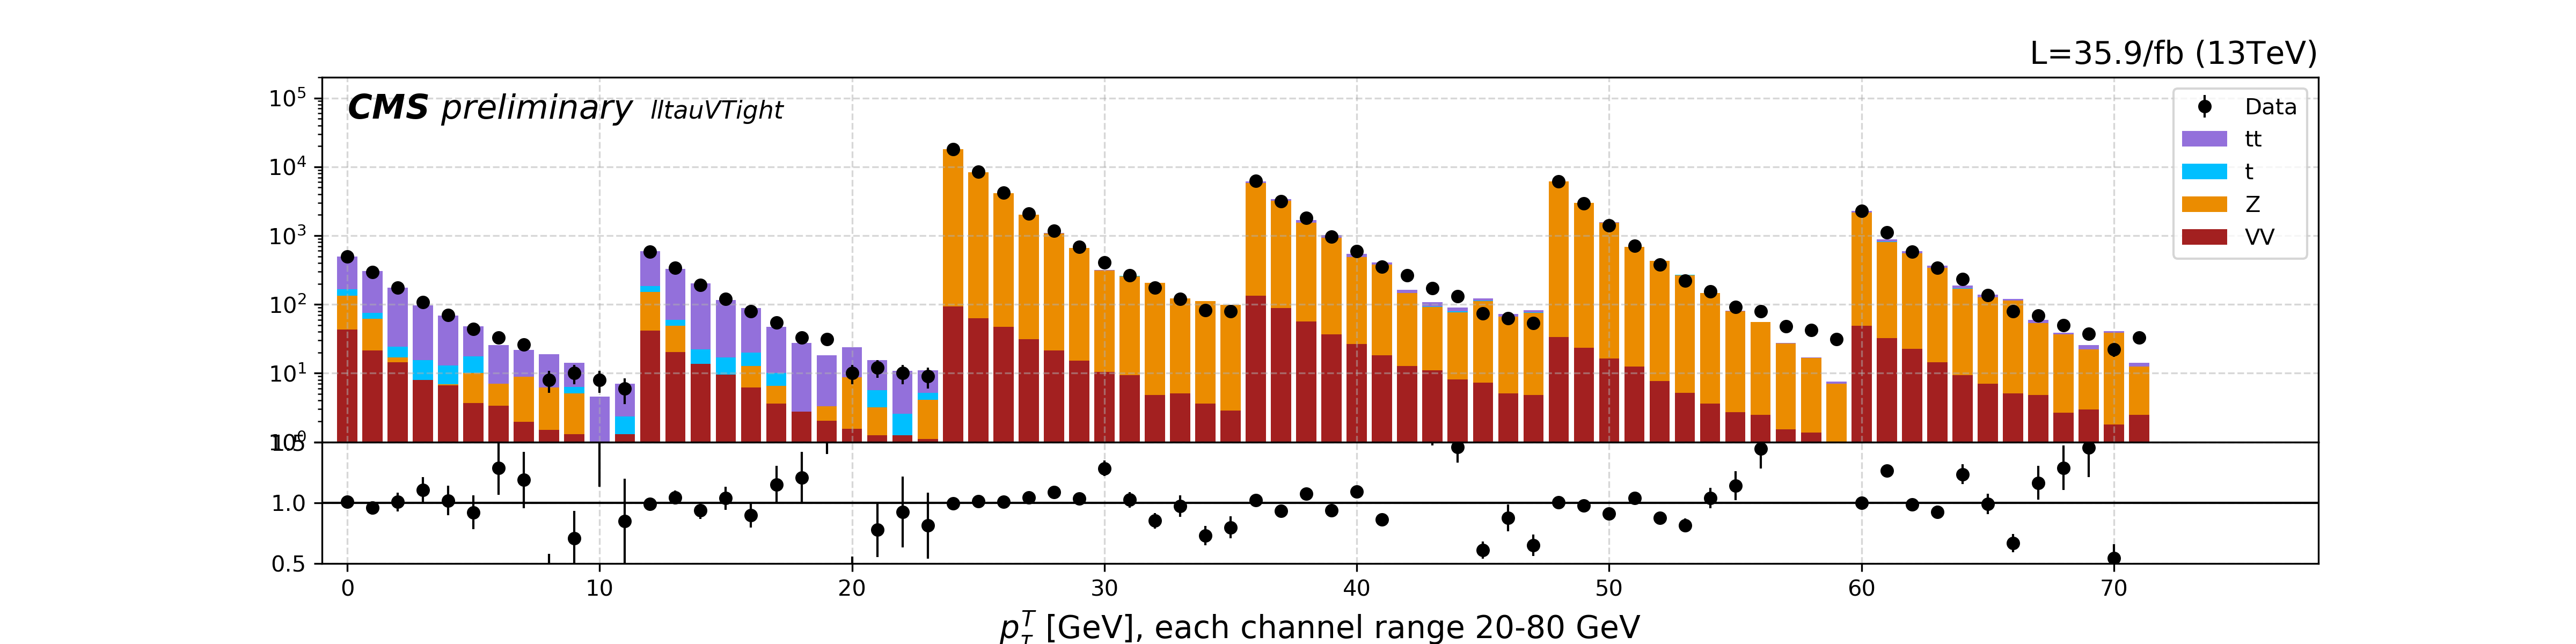
\includegraphics[width=0.99\textwidth]{appendices/jetToTauhReweighting/figures/2020_tauID_postfit_lltauVTight.png}
    \caption{Post distributions}
    \label{fig:appendix:fakeTauId:postfit}
\end{figure}


\begin{figure}
    \centering
    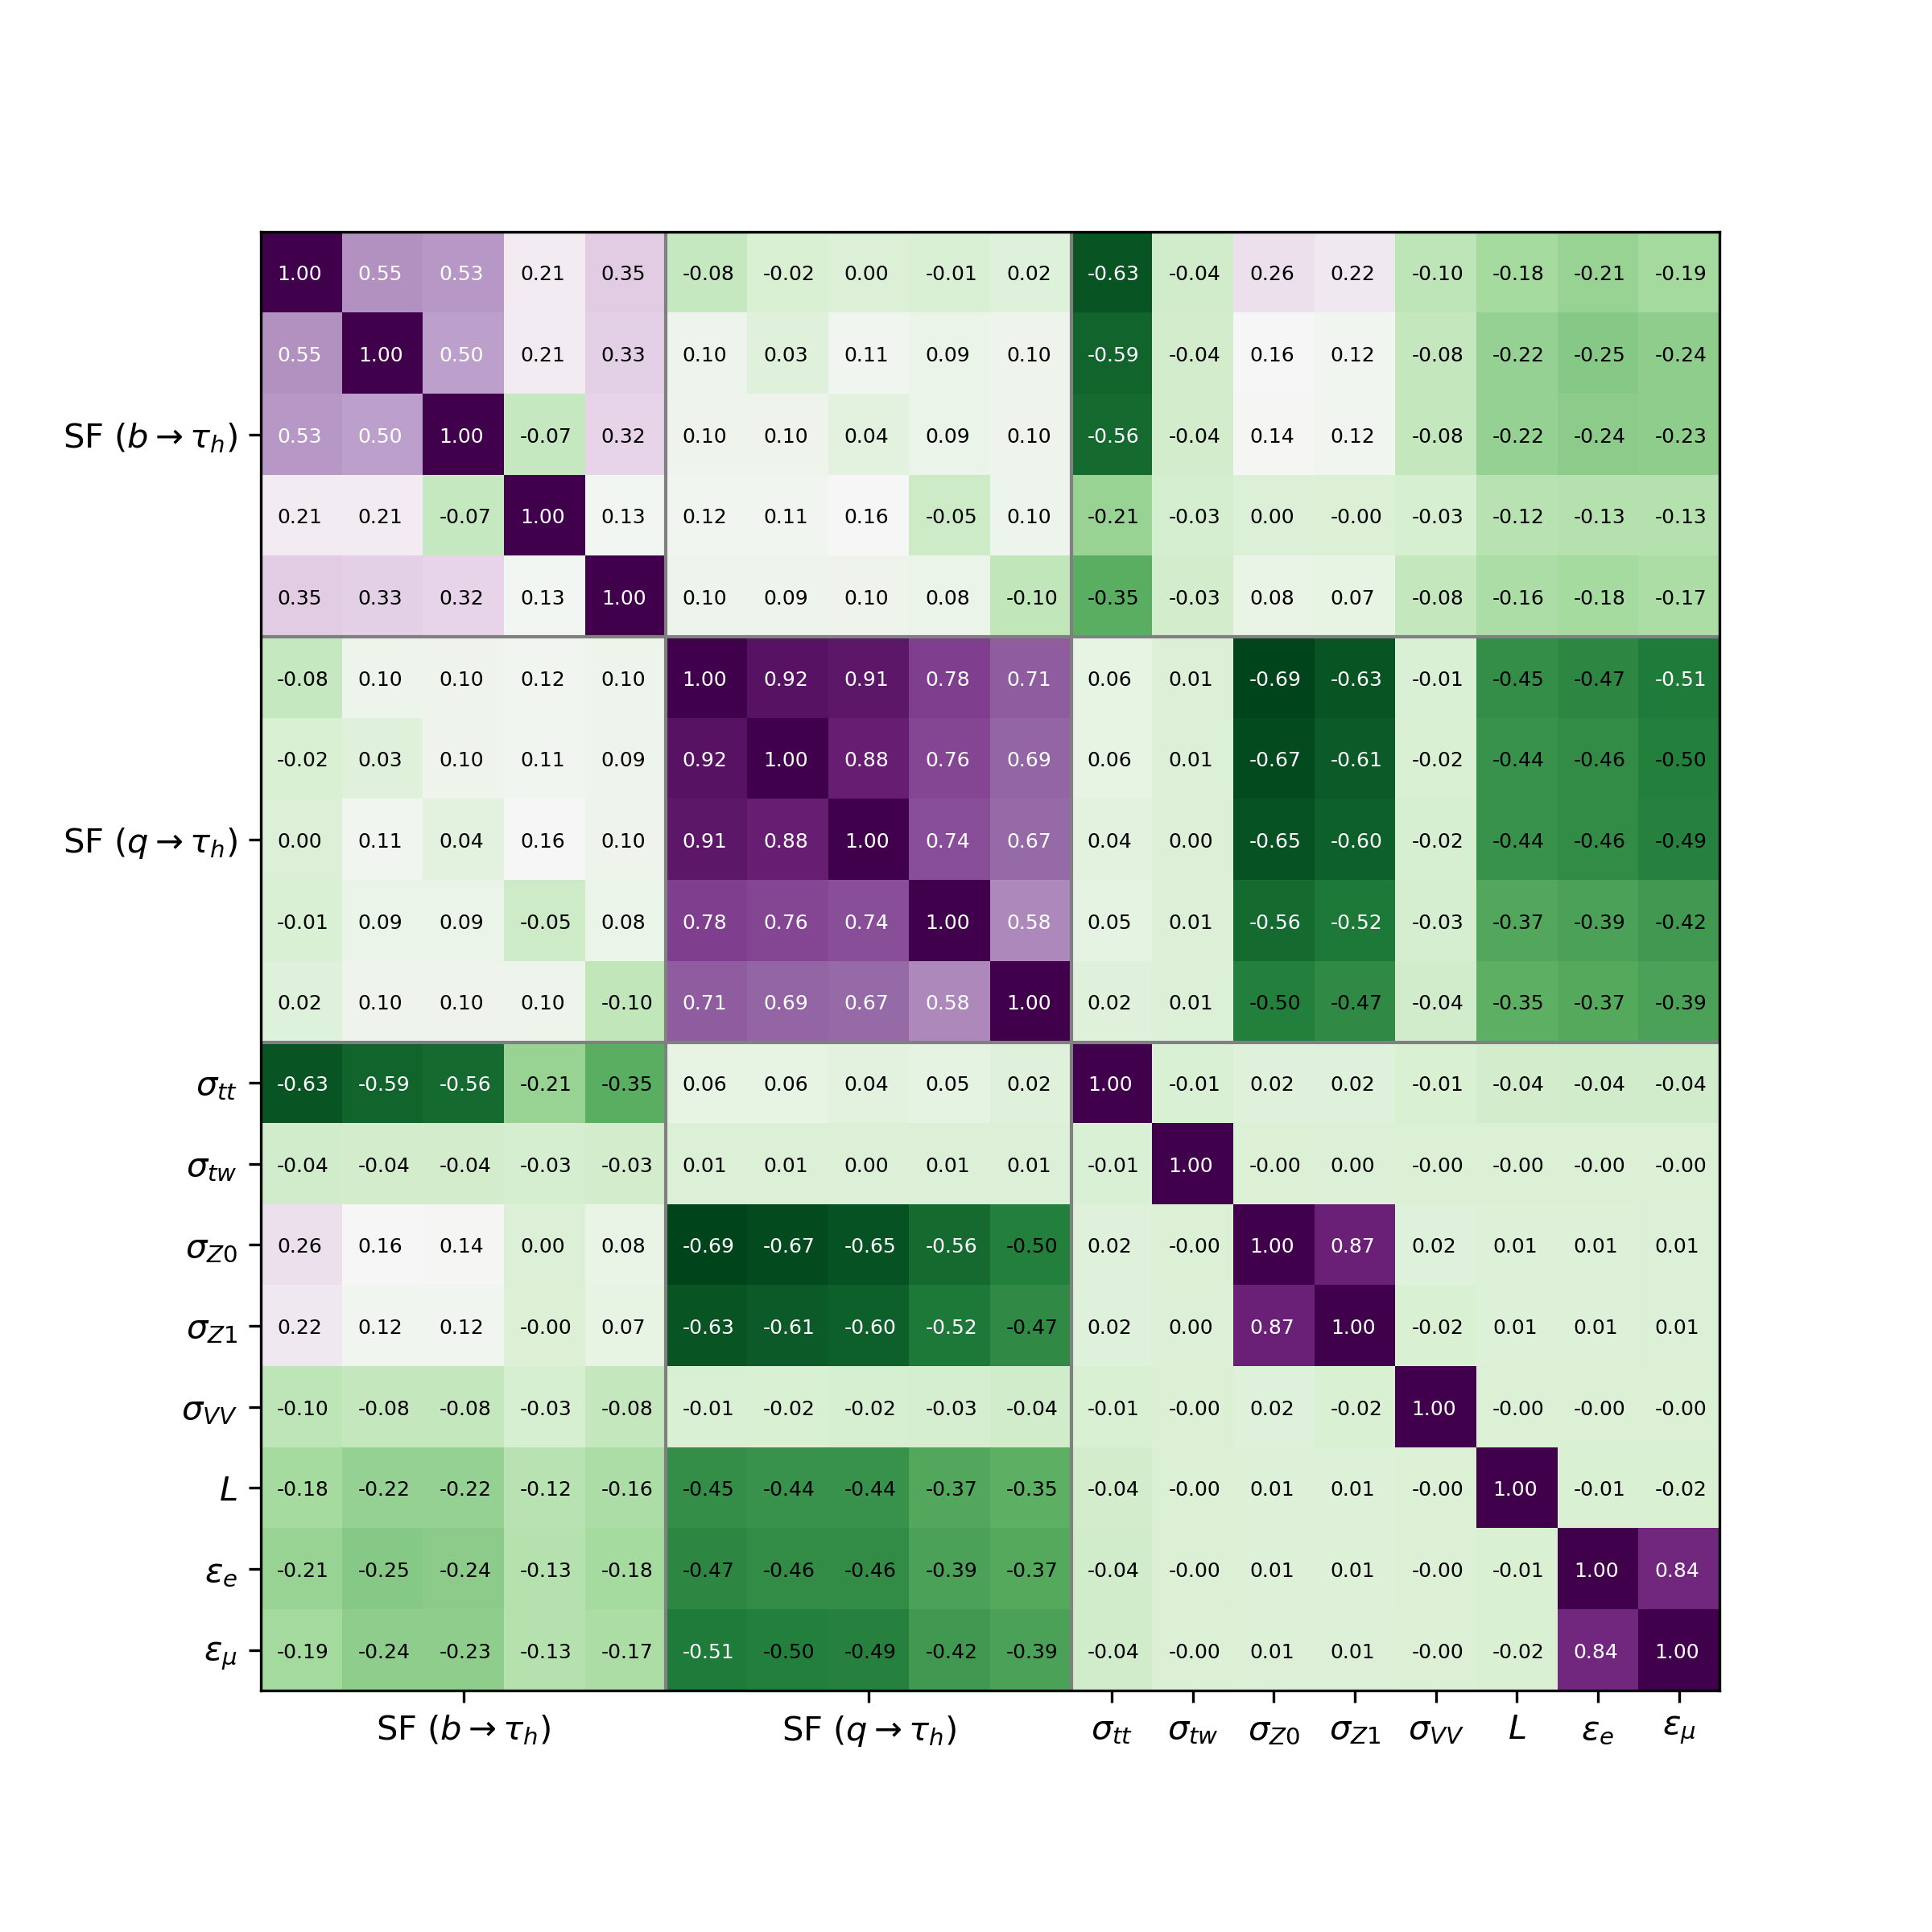
\includegraphics[width=0.49\textwidth]{appendices/jetToTauhReweighting/figures/corr2_lltauTight_splitJetFlavor.png}
    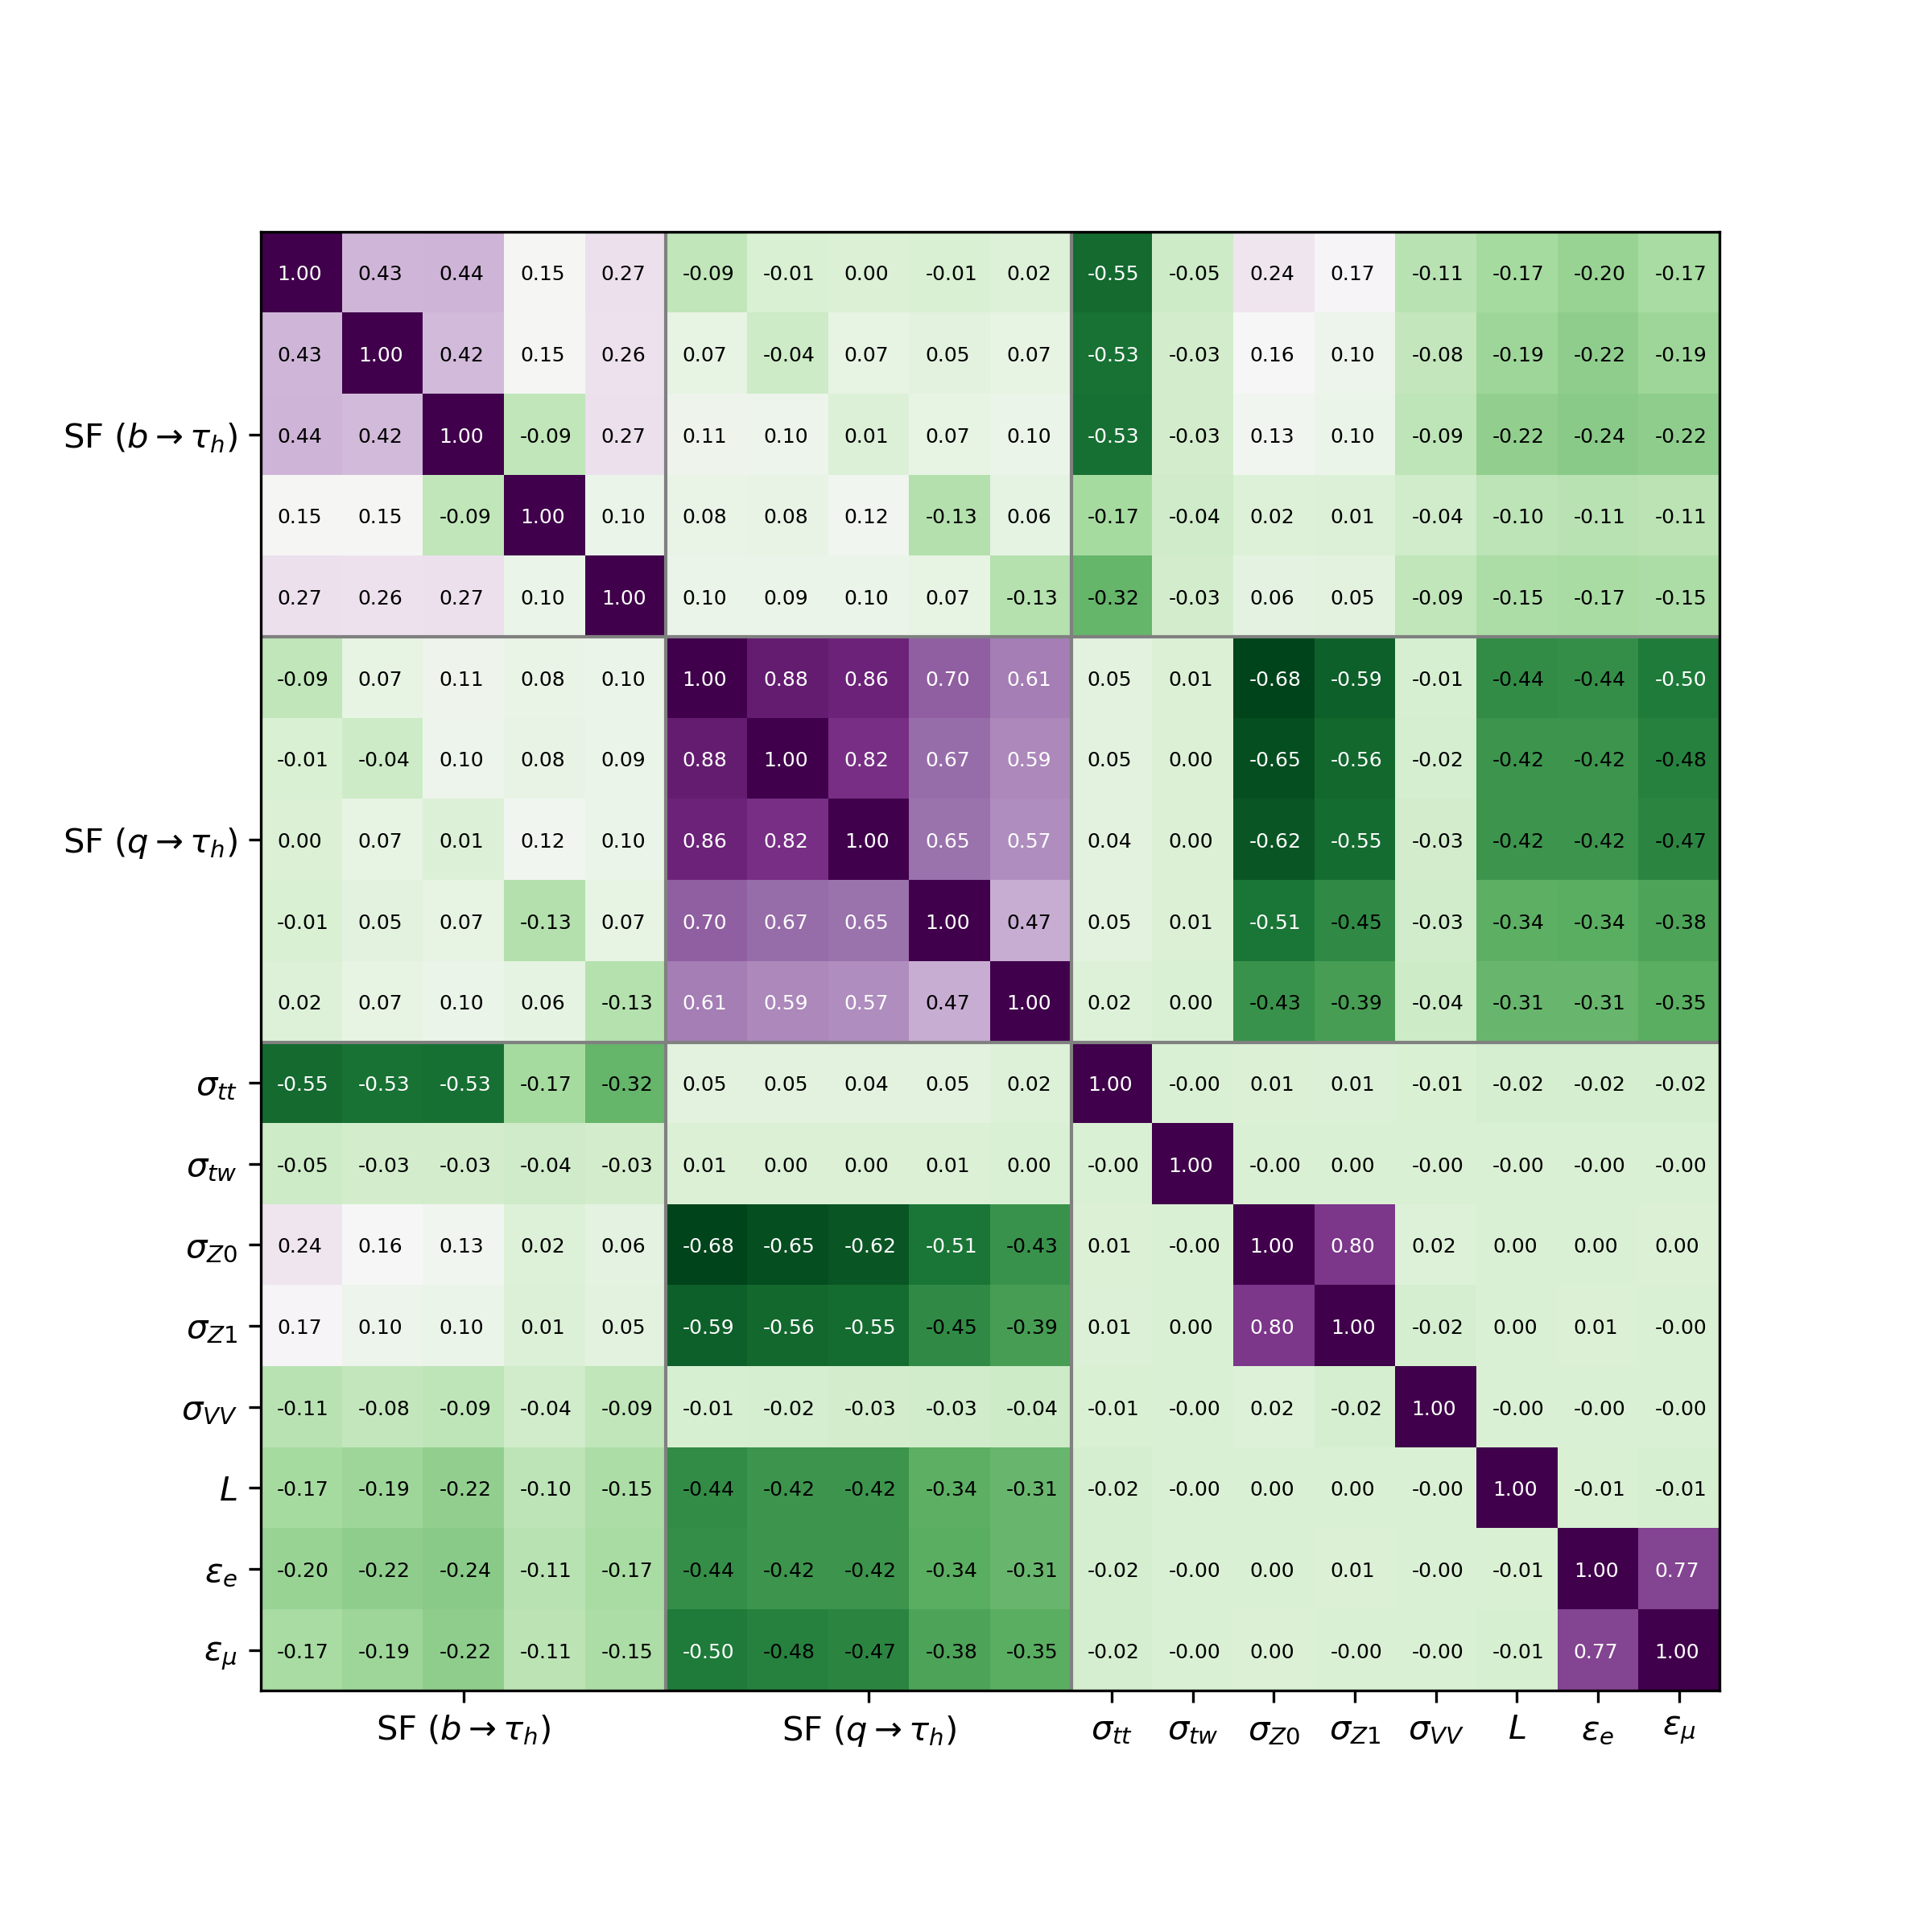
\includegraphics[width=0.49\textwidth]{appendices/jetToTauhReweighting/figures/corr2_lltauVTight_splitJetFlavor.png}
    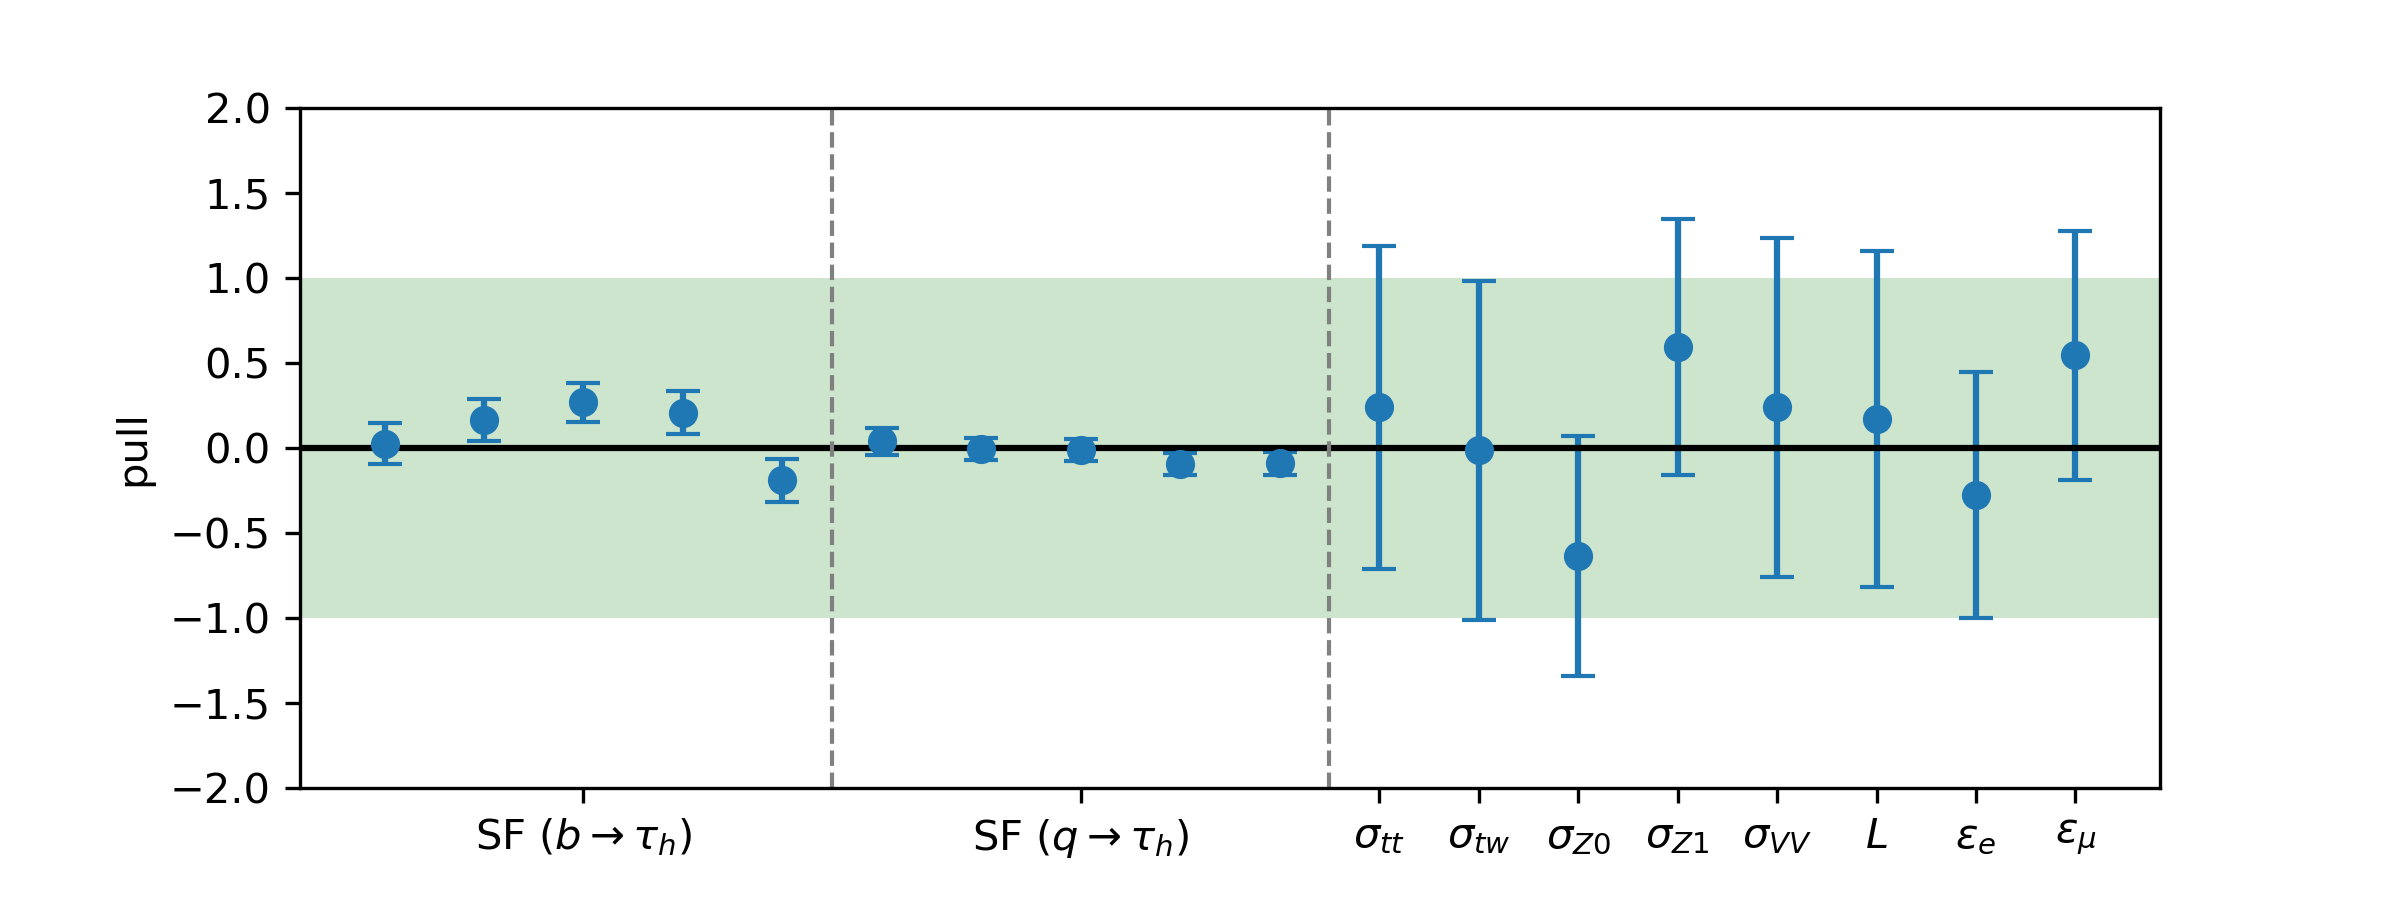
\includegraphics[width=0.49\textwidth]{appendices/jetToTauhReweighting/figures/pull2_lltauTight_splitJetFlavor.png}
    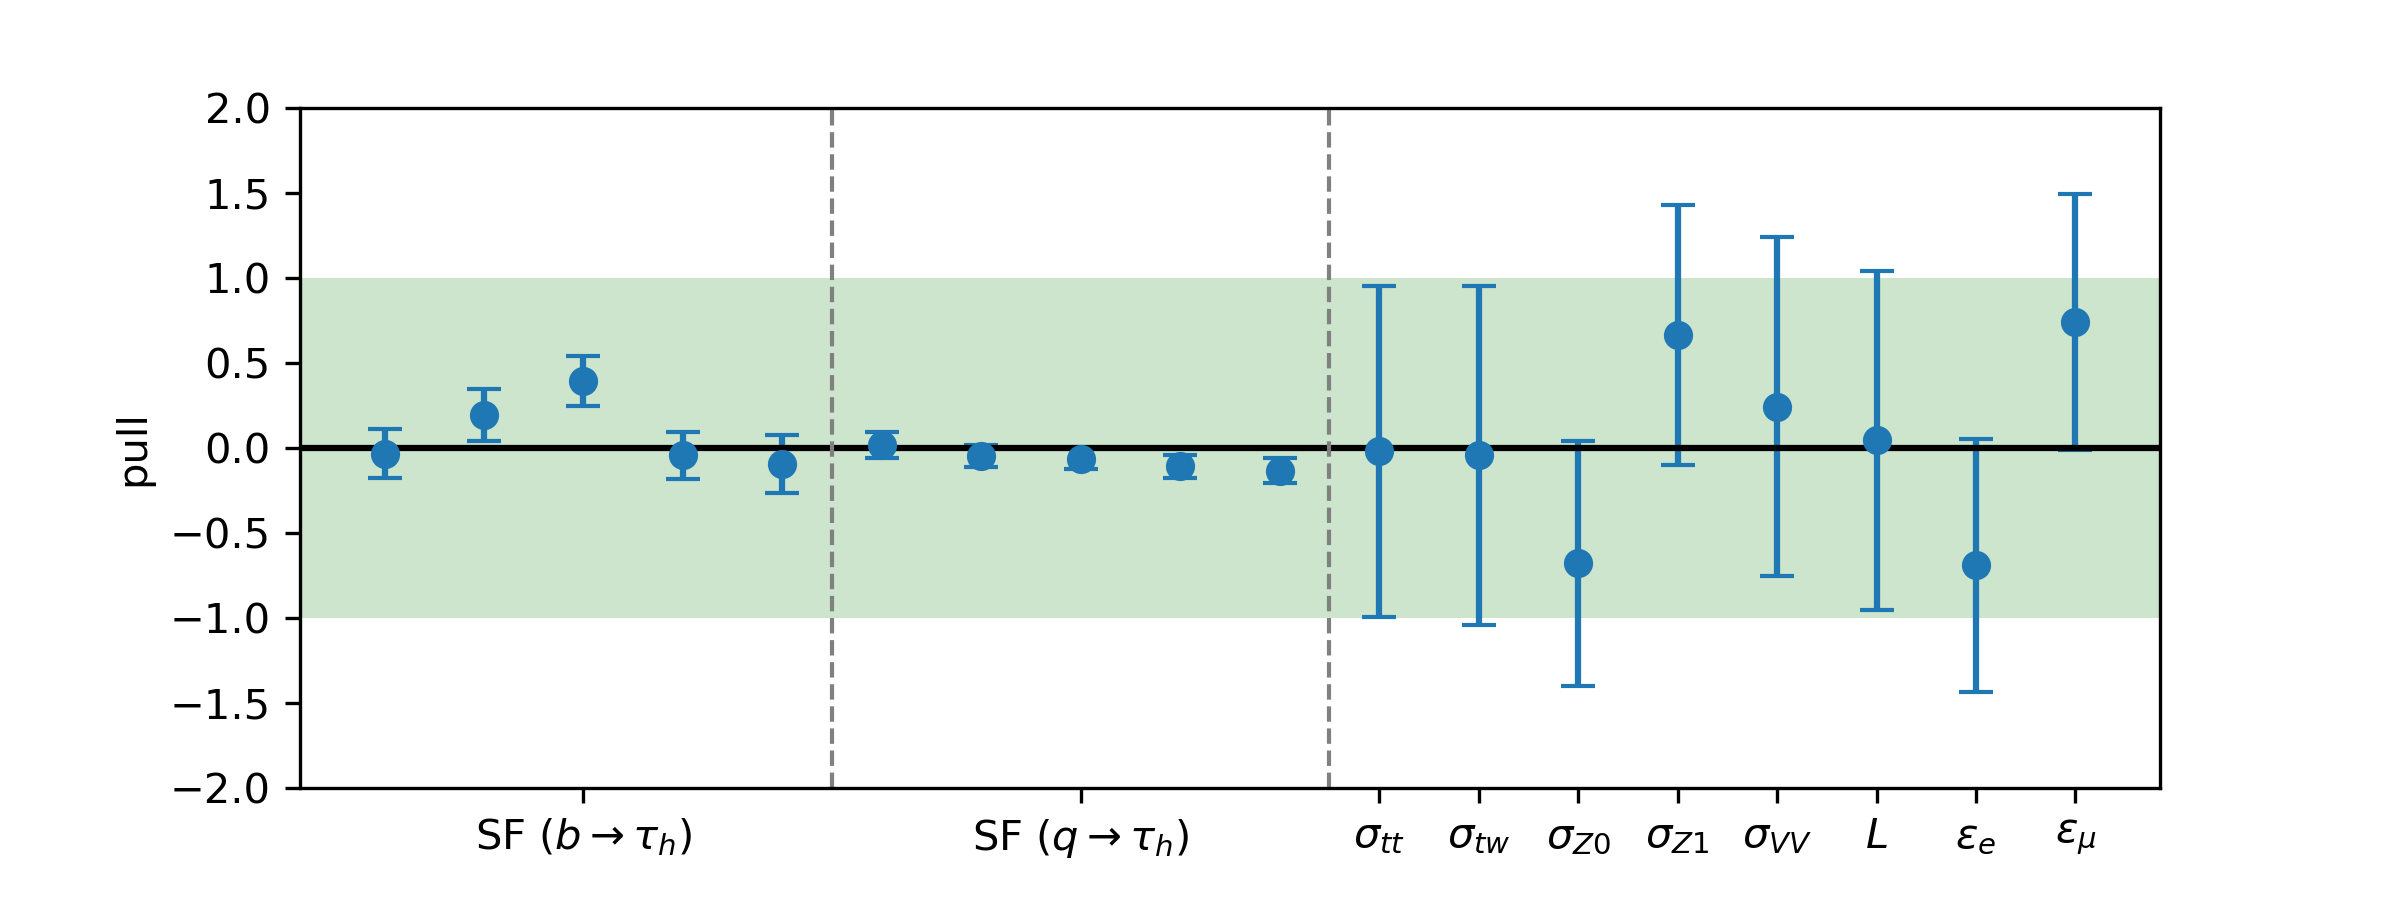
\includegraphics[width=0.49\textwidth]{appendices/jetToTauhReweighting/figures/pull2_lltauVTight_splitJetFlavor.png}
    \caption{The correlation coefficients and pull of fitting parameters}
    \label{fig:appendix:fakeTauId:fitparam}
\end{figure}

\begin{figure}
    \centering
    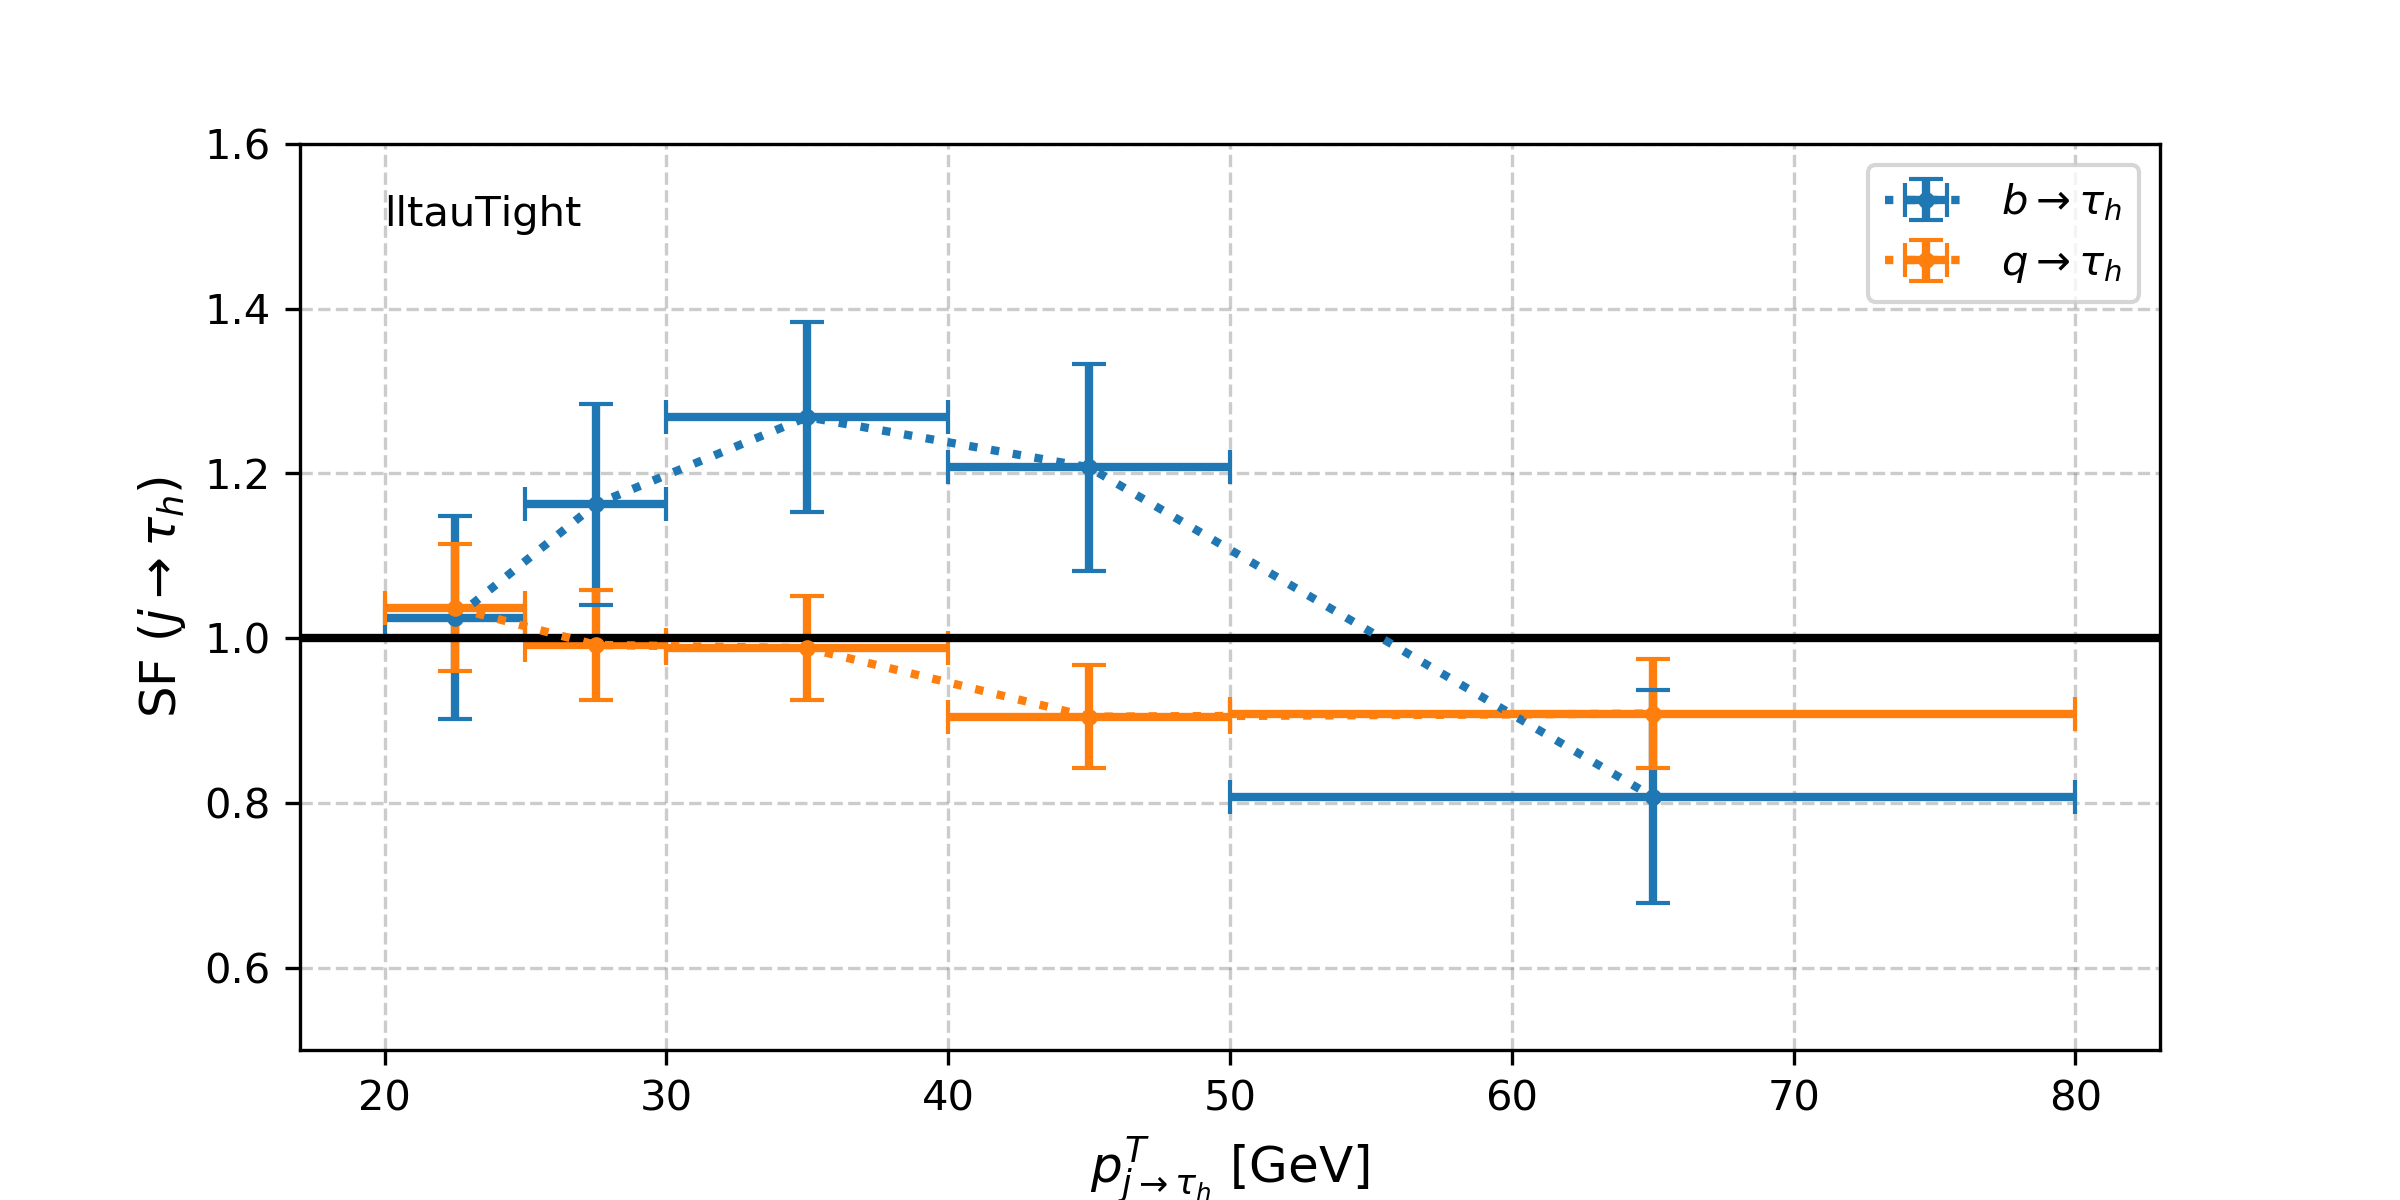
\includegraphics[width=0.49\textwidth]{appendices/jetToTauhReweighting/figures/fit2_ptflavor2_lltauTight.png}
    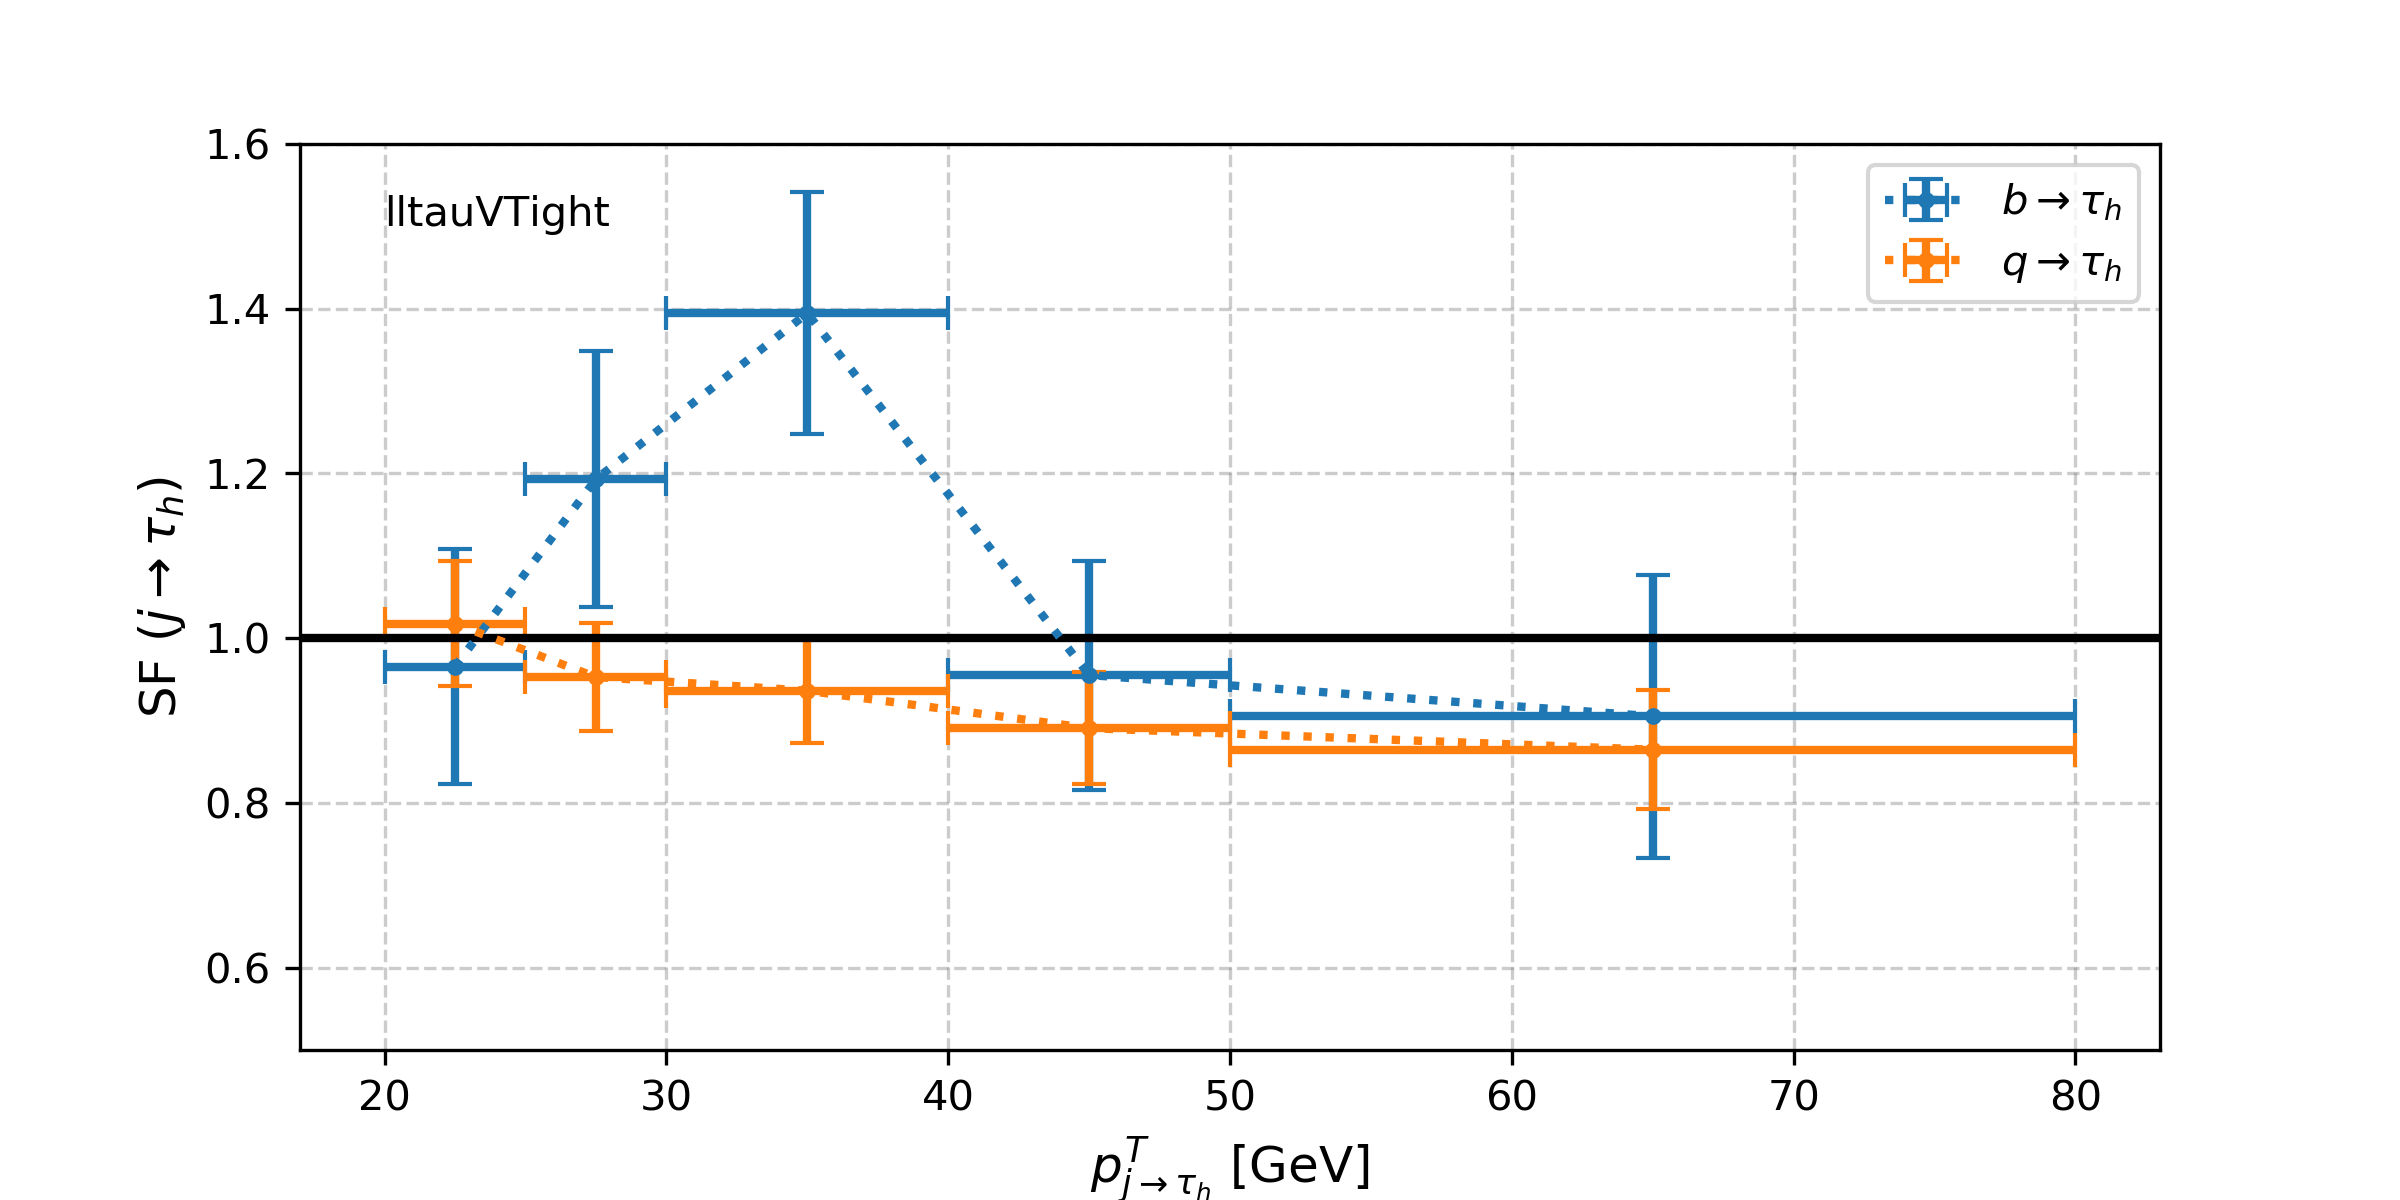
\includegraphics[width=0.49\textwidth]{appendices/jetToTauhReweighting/figures/fit2_ptflavor2_lltauVTight.png}
    \caption{SF}
    \label{fig:appendix:fakeTauId:fit}
\end{figure}

\begin{table}[h]
    \setlength{\tabcolsep}{6pt} % Default value: 6pt
    \renewcommand{\arraystretch}{1.5} % Default value: 1
    \begin{tabular}{c|ccccc}
    \hline
    $p^T_{\tau_h}$ [GeV]  & 20-25         & 25-30         & 30-40         & 40-50         & 50-80         \\
    \hline
    $SF(b\to Tight \cdot \tau_h)$  & $1.02\pm0.12$ & $1.16\pm0.12$ & $1.27\pm0.11$ & $1.21\pm0.13$ & $0.81\pm0.13$ \\
    $SF(q\to Tight \cdot \tau_h)$  & $1.04\pm0.08$ & $0.99\pm0.07$ & $0.99\pm0.06$ & $0.90\pm0.06$ & $0.91\pm0.07$ \\
    \hline
    $SF(b\to VTight \cdot\tau_h)$ & $0.97\pm0.14$ & $1.19\pm0.16$ & $1.39\pm0.15$ & $0.96\pm0.14$ & $0.91\pm0.17$ \\
    $SF(q\to VTight \cdot\tau_h)$ & $1.02\pm0.08$ & $0.95\pm0.07$ & $0.94\pm0.06$ & $0.89\pm0.07$ & $0.86\pm0.07$ \\
    \hline
    \end{tabular}
    \caption{ $SF (j\to \tau_h)$ for Tight and VTight tau MVA}
\end{table}
